% A LaTeX template for MSc Thesis submissions to 
% Politecnico di Milano (PoliMi) - School of Industrial and Information Engineering
%
% S. Bonetti, A. Gruttadauria, G. Mescolini, A. Zingaro
% e-mail: template-tesi-ingind@polimi.it
%
% Last Revision: October 2021
%
% Copyright 2021 Politecnico di Milano, Italy. NC-BY

\documentclass{Configuration_Files/PoliMi3i_thesis}

%------------------------------------------------------------------------------
%	REQUIRED PACKAGES AND  CONFIGURATIONS
%------------------------------------------------------------------------------

% CONFIGURATIONS
\usepackage{parskip} % For paragraph layout
\usepackage{setspace} % For using single or double spacing
\usepackage{emptypage} % To insert empty pages
\usepackage{multicol} % To write in multiple columns (executive summary)
\setlength\columnsep{15pt} % Column separation in executive summary
\setlength\parindent{0pt} % Indentation
\raggedbottom  

% PACKAGES FOR TITLES
\usepackage{titlesec}
% \titlespacing{\section}{left spacing}{before spacing}{after spacing}
\titlespacing{\section}{0pt}{3.3ex}{2ex}
\titlespacing{\subsection}{0pt}{3.3ex}{1.65ex}
\titlespacing{\subsubsection}{0pt}{3.3ex}{1ex}
\usepackage{color}

% PACKAGES FOR LANGUAGE AND FONT
\usepackage[english]{babel} % The document is in English  
\usepackage[utf8]{inputenc} % UTF8 encoding
\usepackage[T1]{fontenc} % Font encoding
\usepackage[11pt]{moresize} % Big fonts

% PACKAGES FOR IMAGES
\usepackage{graphicx}
\usepackage{transparent} % Enables transparent images
\usepackage{eso-pic} % For the background picture on the title page
\usepackage{subfig} % Numbered and caption subfigures using \subfloat.
\usepackage{tikz} % A package for high-quality hand-made figures.
\usetikzlibrary{}
\graphicspath{{./Images/}} % Directory of the images
\usepackage{caption} % Coloured captions
\usepackage{xcolor} % Coloured captions
\usepackage{amsthm,thmtools,xcolor} % Coloured "Theorem"
\usepackage{float}

% STANDARD MATH PACKAGES
\usepackage{amsmath}
\usepackage{amsthm}
\usepackage{amssymb}
\usepackage{amsfonts}
\usepackage{bm}
\usepackage[overload]{empheq} % For braced-style systems of equations.
\usepackage{fix-cm} % To override original LaTeX restrictions on sizes

% PACKAGES FOR TABLES
\usepackage{tabularx}
\usepackage{longtable} % Tables that can span several pages
\usepackage{colortbl}

% PACKAGES FOR ALGORITHMS (PSEUDO-CODE)
\usepackage{algorithm}
\usepackage{algorithmic}

% PACKAGES FOR REFERENCES & BIBLIOGRAPHY
\usepackage[colorlinks=true,linkcolor=black,anchorcolor=black,citecolor=black,filecolor=black,menucolor=black,runcolor=black,urlcolor=black]{hyperref}
\usepackage{cleveref}
%\usepackage[nottoc]{tocbibind}
\usepackage[square, numbers, sort&compress]{natbib} % Square brackets, citing references with numbers, citations sorted by appearance in the text and compressed
\bibliographystyle{abbrvnat} 


% OTHER PACKAGES
\usepackage{pdfpages} % To include a pdf file
\usepackage{afterpage}
\usepackage{lipsum} % DUMMY PACKAGE
\usepackage{fancyhdr} % For the headers
\fancyhf{}
\usepackage{verbatim}
\usepackage{comment}
\usepackage{empheq}   % for boxed numbered equations
%\usepackage[backend=biber, sorting=nty,]{biblatex}

% Input of configuration file. Do not change config.tex file unless you really know what you are doing. 
\input{Configuration_Files/config}

%----------------------------------------------------------------------------
%	NEW COMMANDS DEFINED
%----------------------------------------------------------------------------

% EXAMPLES OF NEW COMMANDS
\newcommand{\bea}{\begin{eqnarray}} % Shortcut for equation arrays
\newcommand{\eea}{\end{eqnarray}}
\newcommand{\e}[1]{\times 10^{#1}}  % Powers of 10 notation

%%%%%%%%%%%%%%%%%%%%%%%%%%%%%%%%%%%%%%%%%%%%%%%%%%%%%%%%%%%%%%%%%%%%%%%%%%%%%%%%%%%%%%%%%%%%%
%                                    BEGIN OF THE DOCUMENT                                  %
%%%%%%%%%%%%%%%%%%%%%%%%%%%%%%%%%%%%%%%%%%%%%%%%%%%%%%%%%%%%%%%%%%%%%%%%%%%%%%%%%%%%%%%%%%%%%


\begin{document}
\let\cleardoublepage\clearpage
\fancypagestyle{plain}{%
\fancyhf{} % Clear all header and footer fields
\fancyhead[RO,RE]{\thepage} %RO=right odd, RE=right even
\renewcommand{\headrulewidth}{0pt}
\renewcommand{\footrulewidth}{0pt}}

%%%%%%%%%%%%%%%%%%%%%%%%%%%%%%%%%%%%%%%%%%%%%%%%%%%%%%%%%%%%%%%%%%%%%%%%%%%%%%%%%%%%%%%%%%%%%
%                                    TITLE PAGE                                          %
%%%%%%%%%%%%%%%%%%%%%%%%%%%%%%%%%%%%%%%%%%%%%%%%%%%%%%%%%%%%%%%%%%%%%%%%%%%%%%%%%%%%%%%%%%%%%

\pagestyle{empty} % No page numbers
\frontmatter % Use roman page numbering style (i, ii, iii, iv...) for the preamble pages

\puttitle{
	title= \centering Superconductivity: \\
    \centering From BCS Theory to Bose-Einstein Condensation of Pairs, % Title of the thesis
	name=Marco Fumagalli, % Author Name and Surname
	course = Phyisics Engineering - Ingegneria Fisica, % Study Programme (in Italian)
	ID  = 10681381,  % Student ID number (numero di matricola)
	advisor= Prof. Silvia Lorenzani, % Supervisor name
	%coadvisor={Name Surname, Name Surname}, % Co-Supervisor name, remove this line if there is none
	academicyear={2025-26},  % Academic Year
} % These info will be put into your Title page 
%%%%%%%%%%%%%%%%%%%%%%%%%%%%%%%%%%%%%%%%%%%%%%%%%%%%%%%%%%%%%%%%%%%%%%%%%%%%%%%%%%%%%%%%%%%%%
%                                    PREAMBLE PAGES                                         %
%%%%%%%%%%%%%%%%%%%%%%%%%%%%%%%%%%%%%%%%%%%%%%%%%%%%%%%%%%%%%%%%%%%%%%%%%%%%%%%%%%%%%%%%%%%%%

\startpreamble
\setcounter{page}{1} % Set page counter to 1

%TO DO!!



%%%%%%%%%%%%%%%%%%%%%%%%%%%%%%%%%%%%%%%%%%%%%%%%%%%%%%%%%%%%%%%%%%%%%%%%%%%%%%%%%%%%%%%%%%%%%
%                                    LISTE OF CONTENTS                                     %
%%%%%%%%%%%%%%%%%%%%%%%%%%%%%%%%%%%%%%%%%%%%%%%%%%%%%%%%%%%%%%%%%%%%%%%%%%%%%%%%%%%%%%%%%%%%%


% TABLE OF CONTENTS
\thispagestyle{empty}
\tableofcontents % Table of contents 
\thispagestyle{empty}
%INDEX DEPTH
%\setcounter{secnumdepth}{1}
%\setcounter{tocdepth}{1}
\cleardoublepage

%%%%%%%%%%%%%%%%%%%%%%%%%%%%%%%%%%%%%%%%%%%%%%%%%%%%%%%%%%%%%%%%%%%%%%%%%%%%%%%%%%%%%%%%%%%%%
%                                    MAIN TEXT                                          %
%%%%%%%%%%%%%%%%%%%%%%%%%%%%%%%%%%%%%%%%%%%%%%%%%%%%%%%%%%%%%%%%%%%%%%%%%%%%%%%%%%%%%%%%%%%%%
% In the main text of your thesis you can write the chapters in two different ways:
%
%(1) As presented in this template you can write:
%    \chapter{Title of the chapter}
%    *body of the chapter*
%
%(2) You can write your chapter in a separated .tex file and then include it in the main file with the following command:
%    \chapter{Title of the chapter}
%    \input{chapter_file.tex}
%
% Especially for long thesis, we recommend you the second option.

\addtocontents{toc}{\vspace{2em}} % Add a gap in the Contents, for aesthetics
\mainmatter % Begin numeric (1,2,3...) page numbering

%%%%%%%%%%%%%%%%%%%%%%%%%%%%%%%%%%%%%%%%%%%%%%%%%%%%%%%%%%%%%%%%%%%%%%%%%%%%%%%%%%%%%%%%%%%%%
%                                    ABSTRACT                                          %
%%%%%%%%%%%%%%%%%%%%%%%%%%%%%%%%%%%%%%%%%%%%%%%%%%%%%%%%%%%%%%%%%%%%%%%%%%%%%%%%%%%%%%%%%%%%%
\input{Abstract/Abstract}

%%%%%%%%%%%%%%%%%%%%%%%%%%%%%%%%%%%%%%%%%%%%%%%%%%%%%%%%%%%%%%%%%%%%%%%%%%%%%%%%%%%%%%%%%%%%%
%                                    CHAPTERS                                          %
%%%%%%%%%%%%%%%%%%%%%%%%%%%%%%%%%%%%%%%%%%%%%%%%%%%%%%%%%%%%%%%%%%%%%%%%%%%%%%%%%%%%%%%%%%%%%
\chapter{Superconductivity}
%================================================================================================
\section{Historical overview}
The phenomenon of \textit{superconductivity} was discovered in 1911 by Heike Kamerlingh Onnes in Leiden, shortly after he succeeded in liquefying helium. His cryogenic laboratory at the University of Leiden was among the first capable of reaching temperatures below \(5\,\mathrm{K}\). While investigating the electrical properties of metals at such low temperatures, Onnes measured the resistivity of \textit{mercury} and found that it dropped abruptly to zero below a critical temperature \( T_c \simeq 4.2\,\mathrm{K} \). 

\begin{figure}[H]
    \centering
    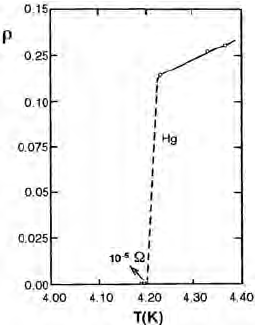
\includegraphics[scale= 0.5]{Chapters/Chapter_1/Images/1_Mercury.png}
    \caption{Temperature dependence of the electrical resistivity of mercury, showing the superconducting transition at \(T_c = 4.2\,\mathrm{K}\).\\
    Image adapted from~\cite{onnes1911}.}
    \label{Figure 1 - Mercury_resistivity}
\end{figure}

This extraordinary result, obtained using liquid helium as a refrigerant, marked the birth of a new state of matter in which electrical currents can flow indefinitely without dissipation.\\
During the following decades, numerous materials were found to exhibit superconductivity (see Fig.~\ref{Figure 2 - Superconductivity_periodic_table}), with transition temperatures gradually increasing as new compounds were discovered. 

\begin{figure}[H]
    \centering
    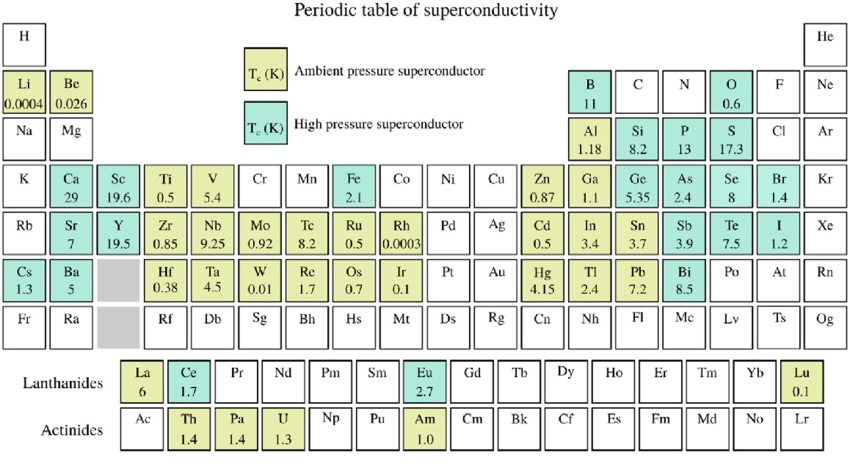
\includegraphics[scale= 0.4]{Chapters/Chapter_1/Images/2_periodic_table.jpeg}
    \caption{Periodic table of superconductivity. Yellow: ambient-pressure; blue: high-pressure superconductors.\\
    Image adapted from~\cite{bennemann2008}.
}
    \label{Figure 2 - Superconductivity_periodic_table}
\end{figure}

By 1980, superconductivity had been observed in many metals and alloys, though notably absent in ferromagnets such as Fe, Ni, or Co, a limitation that we will later understand as a consequence of the interplay between magnetism and electron pairing.
%
%A major milestone was reached with the \textit{A15 compounds} (e.g., Nb\(_3\)Ge), which achieved transition temperatures near \(30\,\mathrm{K}\)~\cite{bennemann2008}. 
%In 1986, Bednorz and M\"uller discovered \textit{high-\(T_c\) cuprate superconductors}, such as La\(_{2-x}\)Ba\(_x\)CuO\(_4\), with \( T_c \approx 35\,\mathrm{K} \), soon followed by YBa\(_2\)Cu\(_3\)O\(_{7-\delta}\) (\( T_c \approx 92\,\mathrm{K} \)) and Hg-based cuprates exceeding \(130\,\mathrm{K}\)~\cite{bednorz1986}. 
%These breakthroughs reshaped condensed-matter physics and revealed that superconductivity could emerge through mechanisms beyond conventional electron–phonon coupling.
%

\section{Experimental Features}
Superconductivity is characterized by two fundamental experimental features that distinguish superconductors from ordinary conductors or semiconductors: \textit{the cancellation of electrical resistivity} and the \textit{Meissner--Ochsenfeld effect}. 
Together, they define superconductivity as a distinct thermodynamic phase of matter.

\paragraph{Zero electrical resistivity.} 
The first distinctive feature of superconductivity is the complete disappearance of electrical resistance below a critical temperature \(T_c\). \\
In normal metals, the temperature dependence of resistivity is described by the
Bloch--Gr\"uneisen relation: it is approximately linear in $T$ at high temperatures
($T \gg \Theta_D$) and follows a $T^5$ law at low temperatures ($T \ll \Theta_D$).
As $T \to 0$ the resistivity saturates to a finite residual value determined by
scattering on lattice defects and impurities, in accordance with Matthiessen's rule.
By contrast, superconductors exhibit a sudden and discontinuous drop of resistivity to exactly zero when cooled below \(T_c\):
\begin{equation}
    \rho\, (T<T_c) = 0.
\end{equation}
This implies the absence of dissipative processes and the ability to sustain persistent currents without decay. 
Experiments have shown that such supercurrents, once induced in a closed superconducting loop, can persist for extremely long timescales (\(\tau \sim 10^5\) years), limited only by external perturbations.\footnote{This phenomenon occurs even in amorphous or polycrystalline materials, demonstrating that superconductivity is not a consequence of lattice perfection but rather an emergent collective quantum property of the electron system.}

\begin{figure}[H]
\centering
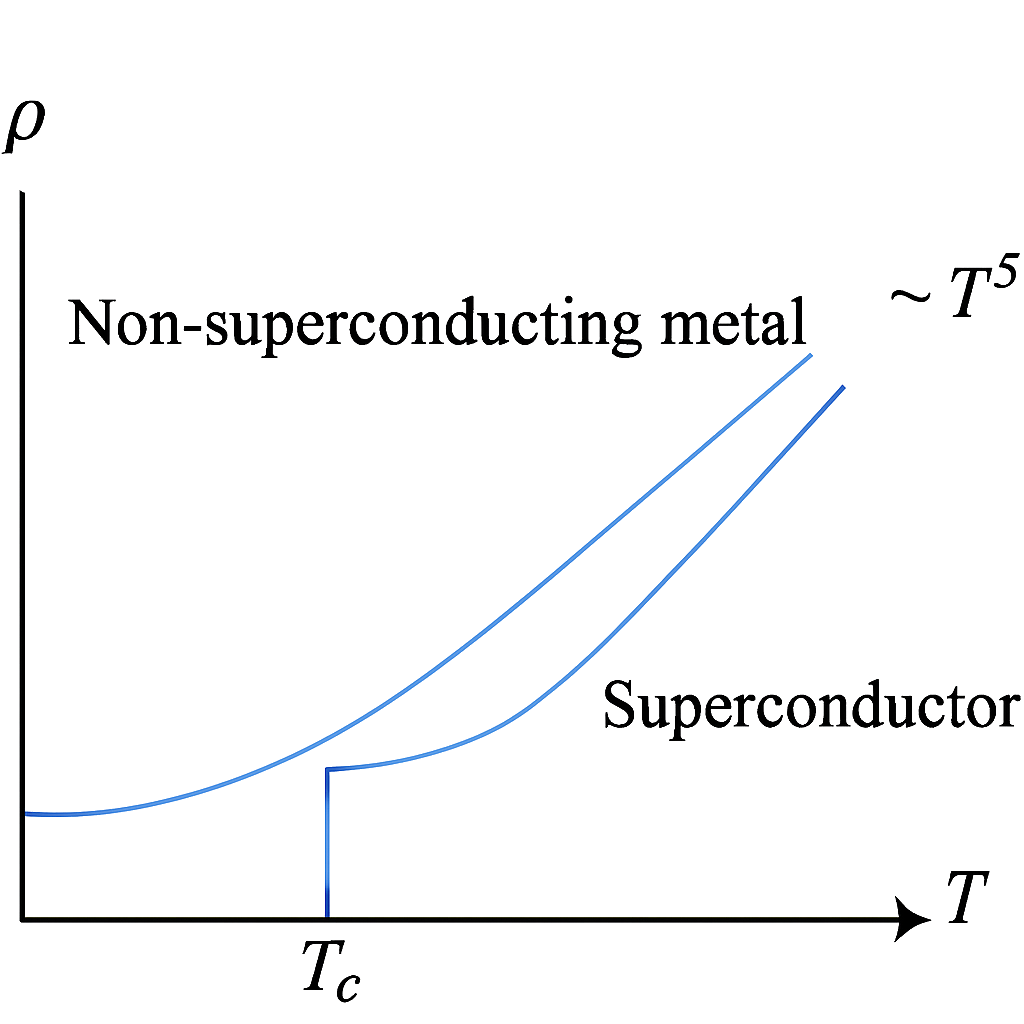
\includegraphics[scale=0.2]{Chapters/Chapter_1/Images/4_zero_res2.png}
\caption{
Temperature dependence of resistivity \(\rho\,(T)\) in a normal metal and in a superconductor. }
\label{fig:resistivity_vs_temperature}
\end{figure}


\paragraph{The Meissner--Ochsenfeld effect.}
The second defining feature of superconductivity, discovered by Meissner and Ochsenfeld in 1933, is the complete expulsion of magnetic flux from the interior of a material upon entering the superconducting state. 
When cooled below \(T_c\) in the presence of an external magnetic field, a superconductor generates surface screening currents that precisely cancel the magnetic field within the bulk, a phenomenon known as the \textit{Meissner effect}. 

This behaviour represents a fundamental distinction from that of a perfect conductor. 
In an ideal conductor with vanishing resistivity $\rho \to 0$, Ohm’s law requires the internal electric field to vanish:
\[
    \mathbf{J} = \sigma \mathbf{E} \quad \implies \quad \mathbf{E} = \rho \mathbf{J}  \underbrace{=}_{\rho \to 0} 0.
\]
From Maxwell’s equation: 
\[
\nabla \times \mathbf{E} = -\frac{\partial \mathbf{B}}{\partial t} 
\quad \iff \quad  
\oint_{\partial S} \mathbf{E} \cdot d\boldsymbol{\ell} = -\frac{d}{dt} \int_{S} \mathbf{B} \cdot d\mathbf{S},
\]
it follows that\footnote{Both the differential and integral forms of Faraday’s law lead to this result, since the integration surface is fixed in time.}
\[
\frac{\partial \mathbf{B}}{\partial t} = 0 
\quad \iff \quad 
\frac{d}{dt} \int_{S} \mathbf{B} \cdot d\mathbf{S} 
=  \frac{d \phi_B(t)}{dt} = 0,
\]
\textit{i.e.}, the magnetic flux within a perfect conductor is therefore conserved or ``\textit{frozen in}''.  
Any attempt to change the magnetic field merely induces surface currents that exactly oppose the variation, maintaining the original flux configuration.

\begin{figure}[H]
\centering
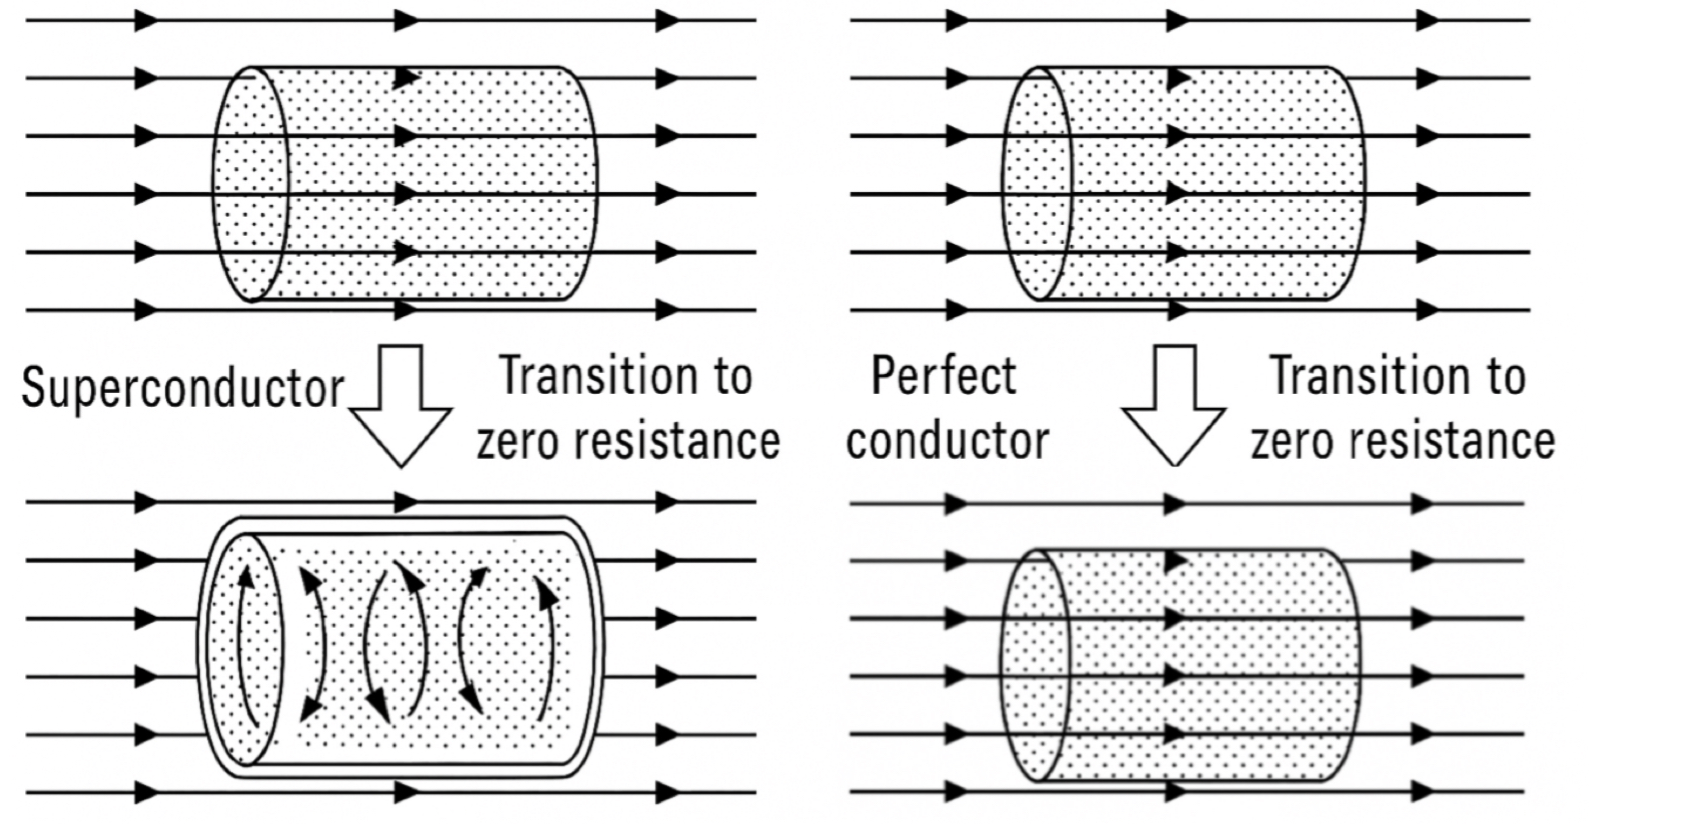
\includegraphics[scale=0.25]{Chapters/Chapter_1/Images/5_m_o.png}
\caption{
Comparison between a superconductor (left) and a perfect conductor (right), both cooled below the critical temperature.
}
\label{fig:meissner_vs_perfect}
\end{figure}

By contrast, in a superconductor the transition into the superconducting state is accompanied by a spontaneous reorganization of the magnetic field: the field is \textit{actively expelled} from the interior, and the magnetic induction decays exponentially from the surface. 
This magnetic screening manifests as perfect diamagnetism\footnote{Complete exclusion of magnetic flux from the interior of a material.}:
\begin{equation}
    \mathbf{B} = \mu_0 (\mathbf{H} + \mathbf{M}) 
    %= \mu_0 \left (1 + \frac{\mathbf{M}}{\mathbf{H}}  \right) \mathbf{H} 
    = \mu_0 \left (1 + \chi_m \right) \mathbf{H} = 0 \quad \implies \quad \chi_m = -1
\end{equation}
This observation cannot be reconciled with classical electrodynamics, confirming that superconductivity represents a new thermodynamic phase rather than a mere extension of perfect conductivity.

It follows that the magnetic field is actively expelled from the interior of a superconductor upon entering the superconducting state.
However, this expulsion is not absolute: the field actually penetrates the surface over a finite distance before decaying exponentially within the material.
This characteristic attenuation length, known as the \textit{penetration depth}, was first introduced by the \textit{London brothers}.


\section{London Equations and Penetration Depth}
\label{Lond_eq}
In 1935, the brothers Fritz and Heinz London proposed a modification of classical electrodynamics in order to account for the electromagnetic behaviour of superconductors, in particular to explain the Meissner--Ochsenfeld effect. 
Their goal was not to alter Maxwell’s equations, which remain valid, but rather to replace Ohm’s law, since the relation between current density and electric field must fundamentally differ in a superconductor. 
%They sought a description compatible with the newly discovered quantum nature of the superconducting state, in which macroscopic coherence plays a central role.

The Londons postulated that charge carriers in the superconducting phase behave as a collective quantum mechanical system described by a macroscopic wavefunction. 
In the ground state, the expectation value of the canonical momentum vanishes, \( \langle \hat{\mathbf{p}} \rangle = 0 \). 
For charge carriers of mass \( M \) and charge \( Q \), the canonical momentum is related to the kinematic momentum by:
\[
    \mathbf{p} = M\mathbf{v} + Q\mathbf{A}(\mathbf{r}),
\]
where \( \mathbf{A}(\mathbf{r}) \) is the magnetic vector potential. 
The canonical momentum is the quantity conjugate to position in the Lagrangian formulation:
\[
    p = \frac{d \mathcal{L}}{d \dot{q}},
\]
while \( M\mathbf{v} \) represents the usual (kinematic) momentum. 
If the expectation value of the canonical momentum vanishes, one obtains:
\[
    M \langle \mathbf{v}_s \rangle = -Q \mathbf{A},
\]
where \( \mathbf{v}_s \) denotes the average velocity of the superconducting carriers. 
The corresponding current density is then:
\begin{equation}
    \mathbf{J}_s = n Q \langle \mathbf{v}_s \rangle = -\frac{n Q^2}{M}\,\mathbf{A},
    \label{000}
\end{equation}
with \( n \) the density of superconducting charge carriers. 
This phenomenological relation constitutes the basis for the \textit{first London equation}, which can be written as:
\begin{equation}
\boxed{
    \mathbf{A} = -\frac{M}{nQ^2}\, \mathbf{J}_s
    }\,.
\end{equation}
Differently from Ohm’s law, which relates the current density to the electric field, the London equation connects the current to the magnetic vector potential.
Because the product \( M / (n Q^2) \) always appears together, it is convenient to introduce a characteristic length scale:
\begin{equation}
\boxed{
    \lambda_L = \sqrt{\frac{M}{\mu_0 n Q^2}}}\, ,
\end{equation}
known as the \textit{London penetration depth}. We'll see that this length quantifies how deep a magnetic field can penetrate into a superconductor before being exponentially attenuated. 
Including the vacuum permeability \( \mu_0 \), the London equation can be recast in the form:
\[
    \mu_0 \mathbf{J}_s = -\frac{1}{\lambda_L^2}\, \mathbf{A}.
\]
Taking the curl of both sides yields the \textit{second London equation}:
\begin{equation}
\boxed{
    \nabla \times \mathbf{J}_s = -\frac{1}{\mu_0 \lambda_L^2}\, \mathbf{B}}\, ,
\end{equation}
where \( \mathbf{B} = \nabla \times \mathbf{A} \) is the magnetic field.
To determine how magnetic fields behave inside a superconductor, we combine this result with Ampère’s law:
\[
    \nabla \times \mathbf{B} = \mu_0 \mathbf{J}_s.
\]

Taking the curl of both sides gives:
\[
    \nabla \times (\nabla \times \mathbf{B}) = \mu_0 (\nabla \times \mathbf{J}_s).
\]

Substituting the second London equation into this expression yields:
\[
    \nabla \times (\nabla \times \mathbf{B}) = -\frac{1}{\lambda_L^2} \mathbf{B}.
\]

Using the vector identity:
\[
    \nabla \times (\nabla \times \mathbf{B}) = \nabla (\nabla \cdot \mathbf{B}) - \nabla^2 \mathbf{B},
\]
and applying Gauss’s law, \( \nabla \cdot \mathbf{B} = 0 \), one obtains:
\[
    -\nabla^2 \mathbf{B} = -\frac{1}{\lambda_L^2}\, \mathbf{B}.
\]

Finally, the London differential equation for the magnetic field takes the form:
\begin{equation}
\boxed{
    \nabla^2 \mathbf{B} = \frac{\mathbf{B}}{\lambda_L^2} \implies \left(\nabla^2 - \frac{\mathbf{1}}{\lambda_L^2}\right) \mathbf{B} = 0}
\end{equation}

This Helmholtz-type equation\footnote{
A \textit{Helmholtz-type equation} is a differential equation of the form 
$(\nabla^2 \pm k^2)\psi = 0$, analogous to the standard Helmholtz equation 
$(\nabla^2 + k^2)\psi = 0$. When the sign is negative, the solutions are exponential rather than oscillatory, 
as in $(\nabla^2 - 1/\lambda_L^2)B = 0$, leading to decaying magnetic fields inside the superconductor.} describes the spatial decay of magnetic fields inside a superconductor.
Its solution\footnote{The solution is presented in the Appendix \ref{app:supercond-derivation}, Section \ref{app:london_derivation}.} 
corresponds to the exponential attenuation:
\begin{equation}
    B(x) = B_0\, e^{-x/\lambda_L},
\end{equation}
showing that magnetic flux penetrates the material only over a finite distance characterized by the London penetration depth \( \lambda_L \).

\begin{figure}[H]
    \centering
    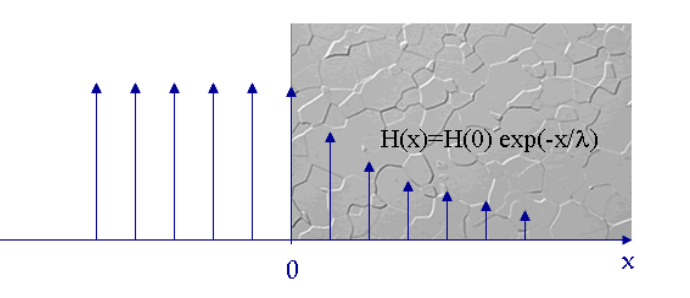
\includegraphics[scale= 0.8]{Chapters/Chapter_1/Images/3_london_depth.png}
    \caption{ An external magnetic field \( H = B/\mu \), applied parallel to the surface of a superconductor, penetrates only a short distance into the material.}
    \label{Figure 3 - London_depth}
\end{figure}

Considering that the London penetration depth $\lambda_L$ typically lies in the range of $10\text{–}100\,\mathrm{nm}$, it is evident that, unless the sample dimensions are of comparable (nanometric) scale, the magnetic flux cannot penetrate the superconductor.

The London theory provided the first quantitative description of the electromagnetic behaviour of superconductors. 
It successfully explained the Meissner effect and introduced the characteristic length scale \( \lambda_L \), which determines how magnetic fields are screened inside the material.\\
Despite its success, the London model remains a purely phenomenological description: it captures how superconductors expel magnetic fields and sustain dissipationless currents, but it does not reveal the microscopic nature of the particles responsible for these effects. In particular, the model assumes the existence of a coherent quantum state without identifying the entities that form it or the mechanism that binds them together.

The next step is therefore to uncover the fundamental constituents of the superconducting condensate.\\
In the following chapter, we turn to the \textit{Bardeen–Cooper–Schrieffer (BCS) theory}, which provides this missing link by showing how electrons near the Fermi surface can attract each other, form bound pairs (\textit{Cooper pairs}) and collectively give rise to the superconducting state.

\chapter{BCS theory}
\label{Ch_2}
\textit{Bardeen--Cooper--Schrieffer (BCS) theory} provides the first microscopic explanation: 
electrons near the Fermi surface form correlated pairs (\textit{Cooper pairs}) that behave effectively as \emph{bosons} and condense into a single macroscopic quantum state. 
\begin{center}
\textit{But electrons repel, how can they pair?}    
\end{center}


\section{Electron-Phonon interaction}
In a metal, electrons interact not only with each other through the Coulomb potential but also with the underlying ionic lattice.
Phonons provide a mechanism through which two electrons can experience an \textit{effective attraction}, despite their mutual repulsion.
This indirect, phonon-mediated attraction constitutes the microscopic origin of pairing in \textit{conventional superconductors}\footnote{Namely those materials that are accurately described by the BCS theory based on electron–phonon coupling.}.\\
By contrast, \emph{unconventional superconductors} (including cuprates, heavy-fermion compounds and some organic materials) cannot be explained solely by phonon-mediated pairing.\footnote{%
Their pairing mechanism likely arises from purely electronic interactions such as spin or charge fluctuations, and their superconducting order parameters often exhibit anisotropic or sign-changing symmetries.%
}

\subsection*{Physical mechanism}
When an electron moves through the crystal lattice, its negative charge slightly attracts the positively charged ions, producing a local distortion of the lattice potential.  
Because the ions are much heavier than the electrons, this deformation relaxes slowly compared to electronic motion.  \\
As the electron passes, the surrounding ions shift slightly towards it. Even after the electron has moved away, the ions relax slowly, producing a temporary region of excess positive charge.
A second electron traveling through the lattice can then be attracted to this residual distortion, effectively feeling a potential well created by the first electron.  
In this way, one electron polarizes the lattice, and another electron is drawn towards this polarization field: the two interact indirectly through the exchange of a \emph{virtual phonon}.  

\begin{figure}[H]
    \centering
    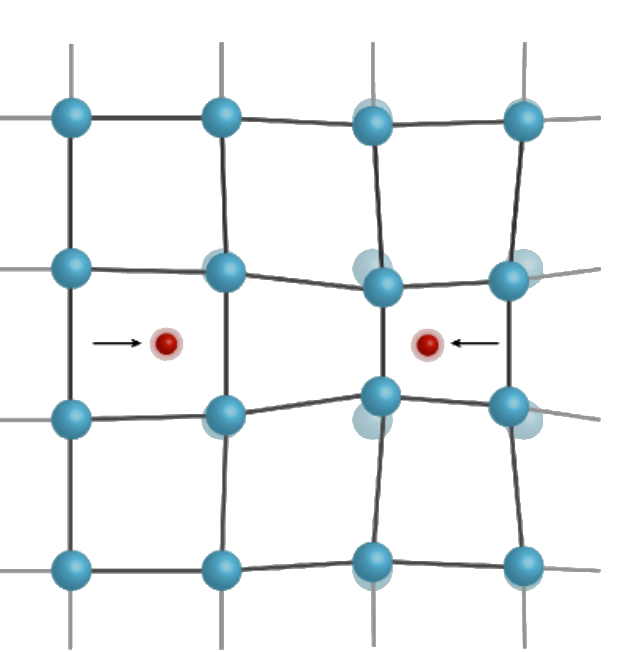
\includegraphics[scale = 0.65]{Chapters/Chapter_3/Images/3_phonon_mediated.png}
    \caption{Schematic representation of the phonon-mediated electron--electron attraction.
    As an electron moves through the lattice, it locally attracts the positively charged ions, creating a distortion that attracts a second electron.}
    \label{fig:phonon_mediated}
\end{figure}

This phonon-mediated process gives rise to an \textit{effective attractive interaction} between electrons, which can overcome their natural Coulomb repulsion under suitable conditions.

\section{Cooper Instability}
Having established that the electron–phonon interaction provides an effective attraction between electrons in a metal, we now turn to its microscopic consequences.\\
Two natural questions arise:

\begin{center}
\textit{Can such an attraction, weak as it may be, lead to the formation of bound states within the Fermi sea?}
\end{center}

and, if so,

\begin{center}
\textit{How does this affect the stability of the normal metallic ground state?}
\end{center}

To address these questions, we begin by considering the simplest possible system: a single pair of electrons interacting through an attractive potential, first in vacuum and then in the presence of a filled Fermi sea.\\
To this end, we first analyze the general two-body interaction problem through the Schrödinger equation, which will form the foundation for the discussion that follows.


\subsection*{Single Cooper Pair}
We begin by studying two electrons interacting via an attractive potential $V(\mathbf{r}_1-\mathbf{r}_2)$, and later apply these results to the cases of vacuum and of a filled Fermi sea.

Consider two electrons interacting via an attractive potential $V(\mathbf{r}_1-\mathbf{r}_2)$.
The two–body Schr\"odinger equation reads:
\begin{equation}
\left[
-\frac{\hbar^2\nabla_{\mathbf{r}_1}^2}{2m}
-\frac{\hbar^2\nabla_{\mathbf{r}_2}^2}{2m}
+ V(\mathbf{r}_1-\mathbf{r}_2)
\right]
\Psi(\mathbf{r}_1,\mathbf{r}_2)
= E\,\Psi(\mathbf{r}_1,\mathbf{r}_2).
\label{eq:cooper_sch}
\end{equation}
Introduce the \textit{centre-of-mass} (COM) and \textit{relative} coordinates as:
\[
\mathbf{R} = \frac{\mathbf{r}_1 + \mathbf{r}_2}{2},
\qquad
\mathbf{r} = \mathbf{r}_1 - \mathbf{r}_2.
\]
In these new variables, the Schrödinger equation~\eqref{eq:cooper_sch} becomes:
\begin{equation}
\left[
-\frac{\hbar^2\nabla_{\mathbf{R}}^2}{2M}
-\frac{\hbar^2\nabla_{\mathbf{r}}^2}{2\mu}
+ V(\mathbf{r})
\right]
\Psi(\mathbf{r},\mathbf{R})
= E\,\Psi(\mathbf{r},\mathbf{R}),
\label{eq:cooper_cm_sch}
\end{equation}
where \(M = 2m\) is the total mass and \(\mu  = m/2\) the reduced mass of the two-electron system.\\
Since the potential depends only on the relative coordinate \(\mathbf{r}\), the COM motion separates from the internal motion.  
We therefore make the ansatz:
\[
\Psi(\mathbf{r},\mathbf{R}) = \psi(\mathbf{r})\, e^{i\mathbf{K}\cdot\mathbf{R}},
\]
where \(\mathbf{K}\) is the total momentum of the pair and \(\psi(\mathbf{r})\) describes the internal structure of the bound state.  
Substituting this form into Eq.~\eqref{eq:cooper_cm_sch} yields the Schrödinger equation for the relative motion:
\begin{equation}
\left[
-\frac{\hbar^2\nabla_{\mathbf{r}}^2}{2\mu}
+ V(\mathbf{r})
\right]\psi(\mathbf{r})
= \tilde{E}\,\psi(\mathbf{r}),
\qquad
\tilde{E} = E - \frac{\hbar^2K^2}{2M}.
\label{eq:cooper_relative_sch}
\end{equation}
where:
\begin{itemize}
    \item \(E\) is the total energy of the two-electron system;
    \item \(\tilde{E} = E_{\mathrm{rel}}\) is the internal (relative-motion) energy associated with the pair’s binding;
    \item \(E_{\mathrm{COM}} = \hbar^2 K^2 / (2M)\) is the kinetic energy of the pair’s centre-of-mass motion, with \(M = 2m\) total mass.
\end{itemize}
The lowest-energy configuration corresponds to $\mathbf{K}=0$, where the total momentum of the pair vanishes and the two electrons have equal and opposite momenta.\\
Depending on the symmetry of the spatial wavefunction, different spin configurations arise in order to preserve the antisymmetry of the total fermionic wavefunction:
\begin{itemize}
    \item If the spatial part is \textit{even}, satisfying $\psi(\mathbf{r}) = \psi(-\mathbf{r})$,  
    the spin part must be \textit{antisymmetric}, corresponding to a \emph{singlet state}:
    \[
    \frac{1}{\sqrt{2}}\left(|\uparrow\downarrow\rangle - |\downarrow\uparrow\rangle\right).
    \]

    \item If the spatial part is \textit{odd}, satisfying $\psi(\mathbf{r}) = -\psi(-\mathbf{r})$,  
    the spin part must be \textit{symmetric}, forming a \emph{triplet state} with three possible spin projections:
    \[
    |\uparrow\uparrow\rangle, \quad
    |\downarrow\downarrow\rangle, \quad
    \frac{1}{\sqrt{2}}\left(|\uparrow\downarrow\rangle + |\downarrow\uparrow\rangle\right).
    \]
\end{itemize}
In conventional superconductors, pairing occurs in the singlet channel, corresponding to even spatial symmetry and opposite spins.

\paragraph{Fourier–space formulation}
To analyse the two-electron bound state it is convenient to work in momentum space.  
Fourier-transforming the relative-coordinate Schr\"odinger equation:
\[
\left[-\frac{\hbar^2\nabla_{\mathbf r}^2}{2\mu}+V(\mathbf r)\right]\psi(\mathbf r)
=\tilde E\,\psi(\mathbf r),
%\label{eq:cooper_relative_sch}
\]
one obtains at the Cooper Integral Equation\footnote{For a full derivation of the Cooper integral equation see Appendix~\ref{app:BCS-derivation}, section \ref{app:cooper_FT}.}:
\begin{equation}
\boxed{
\bigl(\tilde E-2\varepsilon_{\mathbf k}\bigr)\,\psi(\mathbf k)
=\int\!\frac{d^3 k'}{(2\pi)^3}\, V(\mathbf k-\mathbf k')\,\psi(\mathbf k')}\,,
\qquad
\varepsilon_{\mathbf k}=\frac{\hbar^2 k^2}{2m},
\label{eq:cooper_integral_body}
\end{equation}
where the kinetic term becomes diagonal and the interaction appears as a convolution in momentum space.
It is convenient to define:
\[
\Delta(\mathbf k)\equiv \bigl(E-2\varepsilon_{\mathbf k}\bigr)\,\psi(\mathbf k),
\qquad (E\equiv \tilde E\ \text{for }\mathbf K=0),
\]
which yields the compact homogeneous form:
\begin{equation}
\boxed{
\Delta(\mathbf k) = -\!\int\!\frac{d^3 k'}{(2\pi)^3}\;
\frac{V(\mathbf k-\mathbf k')}{\,2\varepsilon_{\mathbf k'}-E\,}\;\Delta(\mathbf k') } \,.
\label{eq:cooper_Delta_body}
\end{equation}
A nontrivial solution $\Delta(\mathbf{k}) \neq 0$ exists only for discrete energies satisfying $E < 2\varepsilon_{\mathbf{k}}$, corresponding to a bound state.
This condition reflects that the total energy of the two interacting electrons is lower than the energy of two independent free electrons, indicating the formation of a stable pair.\\
Thus, the phonon-mediated attraction between electrons therefore provides a microscopic mechanism capable of overcoming their natural Coulomb repulsion.  
%To understand the physical consequences of such an effective interaction, we now turn to the simplest possible system: a single pair of electrons interacting attractively.  
%By solving this two-body problem, we will uncover the essential physics of pairing and establish the foundation for the many-body BCS theory.

\subsection*{Cooper Pair Binding}

We now approach the problem of electron–electron pairing in two steps.  
First, we examine whether a bound state between two electrons can exist in \emph{vacuum} under an attractive interaction.  
Then, we embed the same two-body system in a \emph{metallic environment} (a Fermi sea\footnote{The \textit{Fermi sea} denotes the filled set of single-particle quantum states occupied by fermions up to the Fermi energy \(E_F\) at zero temperature.  
It represents the ground state of a noninteracting Fermi gas, in which all momentum states with \(|\mathbf{k}| \leq k_F\) are occupied, and those above \(k_F\) are empty.  
Excitations or interactions near the Fermi surface (\(|\mathbf{k}| = k_F\)) govern the low-temperature properties of metals and superconductors.%
} of occupied electronic states) and show that this dramatically changes the outcome, leading to what is known as the \textit{Cooper instability}.  

\paragraph{Two-Electron Bound State in Vacuum.}
We first consider the simplest case: two electrons in free space interacting through an effective attractive potential. Our goal is to determine whether such an interaction can lead to the formation of a bound state between the two fermions. We look for an even-parity solution of the relative wavefunction, \(\psi(\mathbf{r}) = \psi(-\mathbf{r})\), which corresponds to antiparallel electron spins and therefore a singlet configuration.  \\
In this scenario, the interaction is modelled in momentum space as a short-ranged potential acting only within a finite energy cutoff defined by the characteristic phonon frequency:
\[
V(\mathbf{k}-\mathbf{k}') =
\begin{cases}
    -V_0 & \text{if } \varepsilon_{\mathbf{k}},\,\varepsilon_{\mathbf{k}'} < \hbar\omega_D,\\[6pt]
    0 & \text{otherwise},
\end{cases}
%\label{eq:V_debye_shell_vac}
\]
where \(V_0 > 0\) measures the strength of the effective attraction and \(\hbar\omega_D\) denotes the Debye energy\footnote{%
The Debye energy \(\hbar\omega_D\) represents the maximum phonon energy in the Debye model of a solid, corresponding to the highest lattice vibrational mode.  
}, corresponding to the maximum phonon energy in the lattice. In this vacuum setting the cutoff simply restricts the interaction to low–energy states:
only single–particle modes with $\varepsilon_{\mathbf k},\varepsilon_{\mathbf k'}<\hbar\omega_D$ contribute, i.e.\ the potential is short–ranged in energy and does not involve high–energy states.\\
Since the potential is constant within the cutoff, the pair wavefunction in momentum space can also be taken as approximately constant, \(\Delta(\mathbf{k}) \simeq \Delta\).  
The integral equation for the two-particle bound state [Eq.~\eqref{eq:cooper_Delta_body}] then reduces to
\[
\Delta = V_0\,\Delta
\int_{\varepsilon_{\mathbf{k}'}<\hbar\omega_D}
\frac{d^3k'}{(2\pi)^3}\, \frac{1}{2\varepsilon_{\mathbf{k}'} - E}.
\]
Because a bound state requires \(\Delta \neq 0\), we can divide both sides by \(\Delta\), yielding
\[
1 = V_0
\int_{\varepsilon_{\mathbf{k}'} < \hbar\omega_D}
\frac{d^3k'}{(2\pi)^3}\,
\frac{1}{2\varepsilon_{\mathbf{k}'} - E},
%\label{eq:self_consistency_vacuum}
\]
where \(E < 0\) denotes the total energy of the pair.  
We now express the momentum integral in terms of the single-particle energy \(\varepsilon\)
using the density of states per spin:
\[
\rho(\varepsilon) =
\frac{1}{4\pi^2}
\left(\frac{2m}{\hbar^2}\right)^{3/2}\!\sqrt{\varepsilon}.
\]
This substitution transforms the integral over momentum space into one over energy:
\[
\int_{\varepsilon_{\mathbf k'}<\hbar\omega_D}
\frac{d^3k'}{(2\pi)^3}
\quad \rightarrow \quad 
\int_0^{\hbar\omega_D} \rho(\varepsilon)\, d\varepsilon,
\]
Thus the Cooper equation becomes
\begin{equation}
\boxed{
1 = V_0 \int_0^{\hbar\omega_D}
\frac{\rho(\varepsilon)\, d\varepsilon}{2\varepsilon - E}}
\label{eq:self_consistency}
\end{equation}
Equation~\eqref{eq:self_consistency} is the \textit{self-consistency condition} for the bound-state energy \(E\):
it expresses the requirement that a nontrivial solution (\(\Delta \neq 0\)) of the Cooper equation
can exist only for specific combinations of the interaction strength \(V_0\) and energy \(E\).\\
Evaluating the integral explicitly:
\[
\int_0^{\hbar\omega_D}\!\!\frac{\sqrt{\varepsilon}\,d\varepsilon}{2\varepsilon - E}
=
\left[
\sqrt{\hbar\omega_D}
- \sqrt{-\frac{E}{2}}\,
\arctan\!\left(\sqrt{\frac{2\hbar\omega_D}{-E}}\right)
\right],
\]
we obtain
\[
1 = V_0\,\frac{1}{4\pi^2}
\left(\frac{2m}{\hbar^2}\right)^{3/2}
\left[
\sqrt{\hbar\omega_D}
- \sqrt{-\frac{E}{2}}\,
\arctan\!\left(\sqrt{\frac{2\hbar\omega_D}{-E}}\right)
\right].
%\label{eq:self_consistency_result}
\]

The right-hand side depends explicitly on the bound-state energy \(E<0\).  
A nontrivial solution exists only if the attractive potential \(V_0\) exceeds a critical threshold.  
Setting \(E \to 0^{-}\) gives the limiting condition:
\begin{equation}
\boxed{
V_{0,\text{min}} = 4\pi^2
\left(\frac{\hbar^2}{2m}\right)^{3/2}
\frac{1}{\sqrt{\hbar\omega_D}}
= \frac{\sqrt{2}\,\pi^2\hbar^3}{m^{3/2}\sqrt{\hbar\omega_D}}}\,.
\label{eq:V0min}
\end{equation}

Hence, in vacuum, a bound state forms only when the attraction is strong enough, \[V_0 > V_{0,\mathrm{min}}.\]  
%This represents the usual molecular binding condition in free space.

\paragraph{Cooper Pairs in a Metal.}
We now place the same two electrons in a \emph{metallic environment}, where all single-particle states are filled up to the Fermi energy \(\varepsilon_F\). In a real metal, only electrons lying close to the Fermi energy are affected by the attractive interaction.
Therefore, the integration range in Eq.~\eqref{eq:self_consistency} is restricted to the \emph{Debye shell},
\(\varepsilon_F < \varepsilon < \varepsilon_F + \hbar\omega_D\),
which contains the electronic states coupled by phonons.
Within this narrow window, the density of states can be approximated by its value at the Fermi level, \(\rho(\varepsilon) \simeq \rho(\varepsilon_F)\), since \(\hbar\omega_D \ll \varepsilon_F\). Only those electrons close to the Fermi surface can participate in the interaction, since phonons couple electronic states within a narrow energy window of width \(\hbar\omega_D\).\\
Thus, we obtain:
\[
1 = V_0\,\rho(\varepsilon_F)
\int_{\varepsilon_F}^{\varepsilon_F+\hbar\omega_D}
\frac{d\varepsilon}{2\varepsilon - E}.
\]
Performing the integration yields
\begin{equation}
\frac{2}{V_0\rho(\varepsilon_F)} =
\ln\!\left(
\frac{2\varepsilon_F - E + 2\hbar\omega_D}{2\varepsilon_F - E}
\right).
\label{eq:cooper_log}
\end{equation}

To express this in terms of the binding energy, we define:
\[
E_b = 2\varepsilon_F - E,
\]
which measures how far the bound-state energy lies below the Fermi level.
Substituting into Eq.~\eqref{eq:cooper_log} gives:
\begin{equation}
\frac{2}{V_0\,\rho(\varepsilon_F)} =
\ln\!\left(\frac{E_b + 2\hbar\omega_D}{E_b}\right).
\label{0123}
\end{equation}
We now make a key assumption at the core of the BCS model: the system is in the \textit{weak-coupling limit}, and we seek non-perturbative solutions in this regime.  
This condition entails:
\begin{itemize}
    \item \(V_0 \rho(\varepsilon_F) \ll 1\), meaning that the effective attractive interaction between electrons is very small compared to the characteristic Fermi energy scale;
    \item Cooper pairs are highly delocalized in real space, with strongly overlapping wavefunctions and weak binding between the constituent electrons.
\end{itemize}
Consequently, the binding energy \(E_b = 2\varepsilon_F - E\) is much smaller than the phonon cutoff energy, \(E_b \ll \hbar\omega_D\).  
In this regime, the logarithm in Eq.\eqref{0123} can be approximated by its dominant term,
\[
\ln\!\left(\frac{E_b + 2\hbar\omega_D}{E_b}\right)
\simeq
\ln\!\left(\frac{2\hbar\omega_D}{E_b}\right),
\]
since the correction proportional to \(E_b\) is negligible. Substituting this approximation back into Eq.~\eqref{0123} yields:
\[
\frac{2}{V_0\rho(\varepsilon_F)}
\simeq
\ln\!\left(\frac{2\hbar\omega_D}{E_b}\right),
\]
which can be inverted to obtain the \emph{binding energy}:
\begin{equation}
\boxed{
E_b = 2\hbar\omega_D\,e^{-\tfrac{2}{V_0\, \rho(\varepsilon_F)}}}\, .
\label{eq:Eb_final}
\end{equation}
\noindent
This result has a profound implication: a bound state can form between two electrons
\emph{for any arbitrarily small attractive potential} (\(V < 0\)).
Such a bound state is known as a \emph{Cooper pair}.
This behaviour contrasts sharply with the free-electron case in vacuum,
where the attractive interaction must exceed a finite threshold to produce a bound state.

In a metal, however, the presence of a well-defined Fermi surface fundamentally changes the situation:
it separates occupied from unoccupied electronic states, creating the conditions under which
even an infinitesimal attraction can lead to the formation of a bound pair.
The existence of this bound state marks the first step towards understanding
the microscopic origin of superconductivity.



%TO DO!! Check whether put it or not

\begin{comment}
\paragraph{Finite momentum and supercurrent}
For a pair with finite centre-of-mass momentum \(\mathbf{K}\), the total energy reads:
\begin{equation}
E = 2\varepsilon_F - E_b + \frac{\hbar^2 K^2}{4m}.
\end{equation}
Thus, in the limit $E \to 2 \varepsilon_F$, the corresponding centre-of-mass momentum and associated current density are:
\begin{equation}
K = \frac{2}{\hbar}\sqrt{mE_b}, 
\qquad
J = n_s e\frac{\hbar K}{m}
= 2n_s e\sqrt{\frac{E_b}{m}},
\end{equation}
where \(n_s\) is the density of superconducting pairs.
This expression connects the microscopic pairing mechanism to the macroscopic flow of supercurrent observed in superconductors.
\end{comment}

%============================== CHECK THIS SECTION ================================ %TO DO!!
\section{Many Cooper Pairs}

In the previous section, we showed that even a very weak attractive interaction can bind two electrons into a correlated pair.  
Such a pair carries total charge \(2e\) and, in the singlet case, total spin zero, so it behaves effectively as a boson.\\
A real superconductor, however, contains not just a single pair but an enormous number of electrons close to the Fermi surface.  
All these electrons experience the same effective attraction and form a highly overlapping collection of Cooper pairs that share a common quantum phase.  
The central idea of BCS theory is that these pairs do not exist as isolated molecules, but as a collective macroscopic quantum state.

In what follows, we will not delve into the full microscopic derivation, whose algebraic steps (mean-field decoupling, Bogoliubov transformation, self-consistency conditions) can be lengthy.
Instead, we present the essential physical picture that captures how a macroscopic number of overlapping Cooper pairs organize into the coherent condensate characteristic of the superconducting state.

\subsection*{Physical picture}

Electrons near the Fermi energy tend to form time-reversed pairs of the form 
\((\mathbf{k}\uparrow,-\mathbf{k}\downarrow)\): they have opposite momenta, opposite spins, and therefore zero total momentum.  
Because the effective attraction is weak, each pair is extremely extended in real space, with a size much larger than the average interparticle spacing.  
As a consequence, different Cooper pairs overlap strongly, and a single electron can simultaneously participate in many pairing configurations.

As will be discussed in the next chapter, a remarkable feature of this regime is that pairing and condensation are inseparable processes:
\[
\text{pair formation} \quad \Longleftrightarrow \quad \text{condensation at } T_c.
\]
The moment the effective attraction destabilizes the Fermi sea, a macroscopic number of overlapping pairs form and collectively lock into a single coherent quantum state.  
It is this collective behaviour, rather than the binding of isolated electron pairs, that gives rise to the superconducting phase.

\paragraph{BCS ground-state wavefunction}
The collective superconducting state is described by the BCS ground-state wavefunction.  
Instead of stating that each momentum state \(\mathbf{k}\) is either filled or empty, BCS theory assigns to it a quantum superposition of the two possibilities.  
The ground state is given by
\begin{equation}
|\Psi_{\mathrm{BCS}}\rangle =
\prod_{\mathbf{k}}
\bigl(u_{\mathbf{k}} + v_{\mathbf{k}}\,
c_{\mathbf{k}\uparrow}^{\dagger}c_{-\mathbf{k}\downarrow}^{\dagger}\bigr)
\,|0\rangle,
\qquad |u_{\mathbf{k}}|^2 + |v_{\mathbf{k}}|^2 = 1.
\label{BCS_groundstate}
\end{equation}

Here:
\begin{itemize}
    \item \(c_{\mathbf{k}\sigma}^{\dagger}\) creates an electron with momentum \(\mathbf{k}\) and spin \(\sigma\);
    \item \(c_{\mathbf{k}\uparrow}^{\dagger}c_{-\mathbf{k}\downarrow}^{\dagger}\) creates a Cooper pair with zero total momentum;
    \item \(u_{\mathbf{k}}\) and \(v_{\mathbf{k}}\) are the amplitudes for the pair state \((\mathbf{k},-\mathbf{k})\) to be empty or occupied;
    \item \(|0\rangle\) denotes the filled Fermi sea of the normal state.
\end{itemize}

Each factor \((u_{\mathbf{k}} + v_{\mathbf{k}} c_{\mathbf{k}\uparrow}^{\dagger}c_{-\mathbf{k}\downarrow}^{\dagger})\)  
represents a coherent superposition of “no pair in mode \(\mathbf{k}\)” and “one Cooper pair in mode \(\mathbf{k}\)”.  
The full superconducting ground state is the product of these contributions, forming a condensate of Cooper pairs all sharing the same global phase.

This structure makes the connection with Bose--Einstein condensation explicit:  
Cooper pairs with zero total momentum occupy a common coherent quantum state,  
but with a momentum-dependent weight \(v_{\mathbf{k}}\) rather than populating a single momentum mode.

\bigskip
Up to this point, we have established the microscopic mechanism responsible for the formation of Cooper pairs.\\  
However, the emergence of superconductivity as a macroscopic quantum phenomenon requires understanding how these pairs collectively condense into a coherent quantum state.  
To address this, in the next chapter we turn to the concept of \textit{Bose–Einstein condensation}, which describes the collective behaviour of these composite bosons.









\begin{comment}
%============================== CHECK THIS SECTION ================================ TO DO!!
%============================== CHECK THIS SECTION ================================
%============================== CHECK THIS SECTION ================================
\section{The BEC--BCS Crossover}
\label{sec:BEC-BCS-crossover}

The BCS and BEC descriptions represent two complementary limits of the same underlying phenomenon---the condensation of paired fermions.  
In the \emph{BCS limit}, the attraction between electrons is weak and their pairs are highly overlapping, forming a collective quantum state characterized by long-range phase coherence but little spatial localization.  
In the \emph{BEC limit}, the attraction becomes strong enough to form tightly bound pairs behaving as independent bosons that undergo Bose--Einstein condensation.  
Between these two limits lies a smooth, continuous evolution known as the \emph{BEC--BCS crossover}.

As the interaction strength increases, the \textit{pair size} $\xi_{\mathrm{pair}}$ gradually decreases from much larger than the average inter-particle spacing ($\xi_{\mathrm{pair}} \gg n^{-1/3}$) in the BCS regime, to much smaller than it ($\xi_{\mathrm{pair}} \ll n^{-1/3}$) in the BEC regime.  
Concurrently, the \textit{chemical potential} $\mu$ evolves from approximately the Fermi energy ($\mu \approx \varepsilon_F$) in the weak-coupling limit to negative values ($\mu \approx -E_b/2$) characteristic of bound molecules in the strong-coupling limit.  
Despite these microscopic changes, the transition is \emph{continuous}: there is no phase boundary separating BCS and BEC superconductivity.  
Both phases share the same broken $\mathrm{U}(1)$ gauge symmetry and are described by a common complex order parameter:
\[
\Delta = |\Delta|\,e^{i\phi},
\]
which reflects the global phase coherence of the condensate.\\
The unified picture is therefore that of a single condensate whose microscopic nature evolves smoothly with interaction strength:
\[
\text{BCS: overlapping pairs, }\mu > 0
\;\longleftrightarrow\;
\text{BEC: bound molecules, }\mu < 0.
\]
In real materials, such as high-$T_c$ cuprates or ultracold Fermi gases, the physical regime often lies in between these two extremes.  
Here, pairing and condensation occur on comparable energy scales---a situation referred to as the \emph{intermediate-coupling regime}.  
This region is of particular interest because it combines the strong pairing tendency of the BEC side with the long-range coherence of the BCS side, potentially accounting for the enhanced critical temperatures observed experimentally.

\end{comment}
\chapter{Bose-Einstein condensation} 
\label{chapter3}
%===============================================================================================
\section{Historical foundation} %TO DO!! Check the title 
The concept of \textit{Bose--Einstein condensation} (BEC) originates from the early development of quantum statistics in the 1920s.  
In 1924, \textit{Satyendra Nath Bose} introduced a new counting rule for indistinguishable photons, leading to what is now known as \textit{Bose--Einstein statistics}.  
Shortly after, \textit{Albert Einstein} extended Bose's formalism to a gas of material particles obeying the same statistics (bosons).  
Einstein predicted that, below a certain critical temperature \( T_c \), a macroscopic fraction of these particles would accumulate in the lowest quantum state of the system, producing a new phase of matter characterized by long-range quantum coherence\footnote{%
Long-range quantum coherence refers to the property whereby the quantum phases of individual particles become correlated across macroscopic distances.  
As a result, the entire system can be described by a single complex wavefunction with a well-defined global phase.}.  
For decades, this prediction remained purely theoretical.

Only in 1995 was Bose--Einstein condensation realized experimentally in dilute atomic gases by \textit{Cornell} and \textit{Wieman} (rubidium) and by \textit{Ketterle} (sodium), achievements that earned them the Nobel Prize in Physics in 2001.  
These experiments confirmed the existence of a macroscopic quantum state at ultralow temperatures, with a sharply peaked momentum distribution indicating the population of a single ground-state wavefunction.  
From a physical standpoint, the condensate can be viewed as a collection of bosons occupying the same single-particle state, described by a common wavefunction, below a critical temperature \( T_c \).  


\section{Bose--Einstein distribution}
The quantum statistical behaviour of bosons differs fundamentally from that of classical particles.\\
Because bosons are indistinguishable and do not obey the Pauli exclusion principle\footnote{Formulated by Wolfgang Pauli in 1925, the Pauli exclusion principle states that two identical fermions cannot occupy the same quantum state simultaneously. This rule follows from the antisymmetric nature of the fermionic wavefunction under particle exchange.}, any number of them can occupy the same quantum state.
For a system in thermal equilibrium, the average occupation number of a single-particle energy level \( \varepsilon_i \) is given by the \textit{Bose--Einstein distribution}\footnote{Throughout this work, the same function will also be denoted as $f(\varepsilon)$.}:
\begin{equation}
    \langle n_i \rangle = \frac{1}{e^{\beta(\varepsilon_i - \mu)} - 1},
    \label{eq:BE_distribution}
\end{equation}
where \( \beta = 1/(k_B T) \) is the Boltzmann factor\footnote{More generally, \( \beta \) is defined as the \textit{thermodynamic beta}, a numerical quantity related to the system’s temperature that establishes a connection between the statistical and thermodynamic descriptions of a system.} and \( \mu \) is the chemical potential.  

\begin{figure}[H]
    \centering
    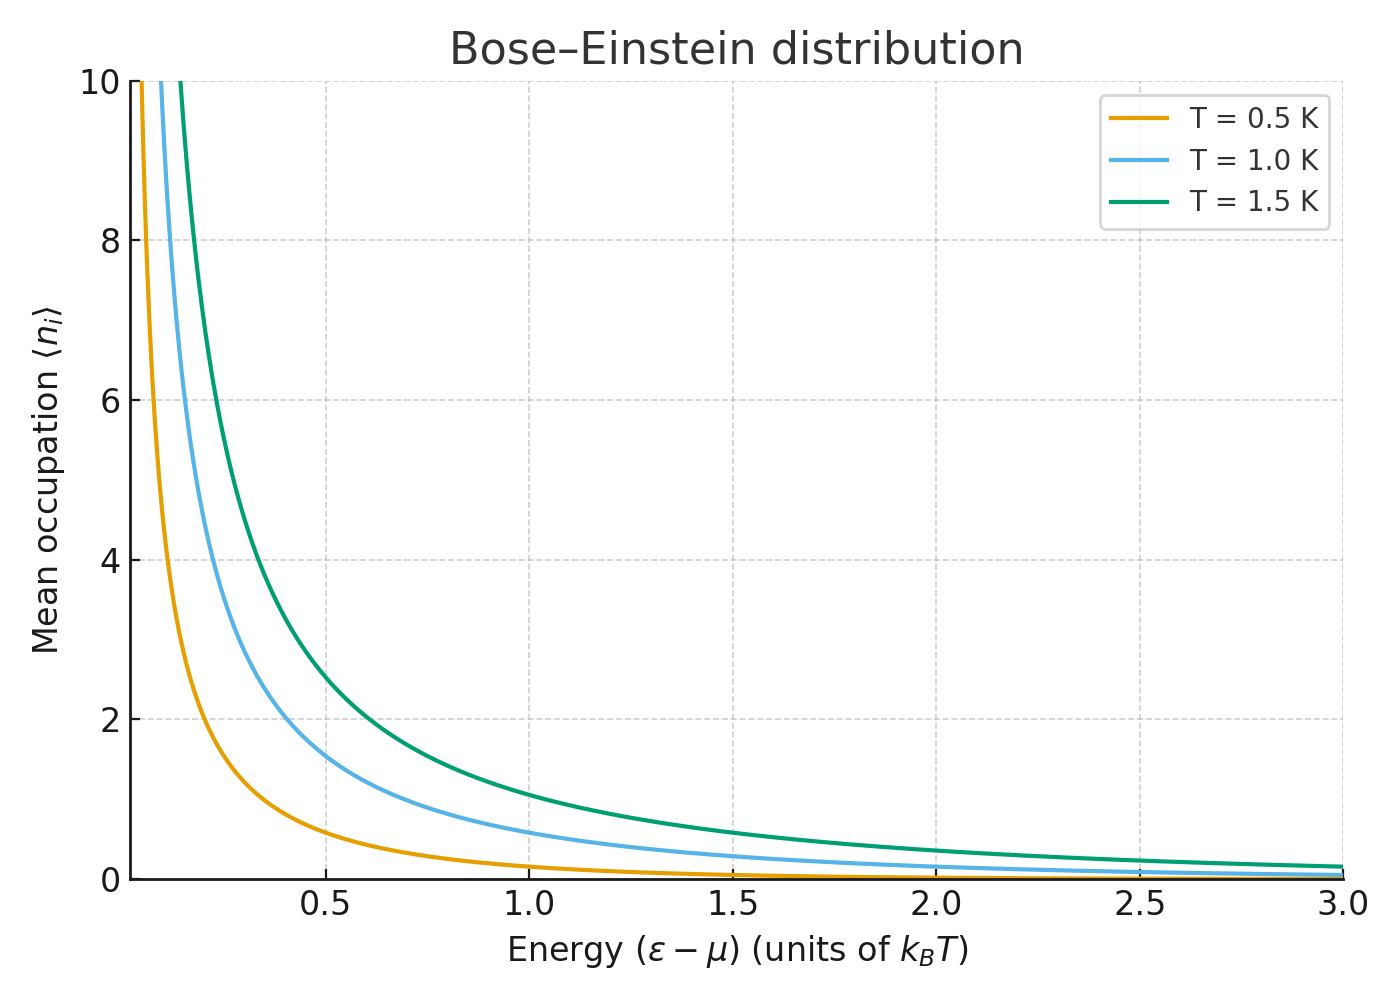
\includegraphics[scale= 0.6]{Chapters/Chapter_2/Images/1_Bose_einstein.png}
    \caption{Bose-Einstein distribution: the mean occupation number \( \langle n_i \rangle \) is shown as a function of the normalized energy \( (\varepsilon - \mu)/(k_B T) \) for three temperatures.}
    \label{Figure 4 - Bose_Einstein_distribution}
\end{figure}

As the temperature decreases, the system departs from classical behaviour.  
The chemical potential \( \mu \) increases towards zero (\( \mu \to 0^- \)), and the denominator in Eq.~\eqref{eq:BE_distribution} becomes small for low-energy states.  
When \( \varepsilon \approx \mu \), the exponential approaches unity and the occupation number diverges:
\[
    \langle n_i \rangle \rightarrow \infty.
\]
This divergence indicates that an increasingly large fraction of bosons accumulate in the lowest-energy state of the system. At sufficiently low temperature, this results in a macroscopic occupation of the ground state. In the extreme limit \( T \to 0 \), all particles occupy the ground state.

\subsection*{Classical limit}
In the limit of high temperature or low density, the system behaves classically.  
When the term \( \beta(\varepsilon - \mu) \gg 1 \), the exponential dominates over unity, so that:
\[
    e^{\beta(\varepsilon - \mu)} \gg 1 \quad \Rightarrow \quad 
    \langle n_i \rangle \approx e^{-\beta(\varepsilon_i - \mu)}.
\]
This corresponds to the \textit{Maxwell--Boltzmann distribution}, which governs classical particles.  
In this regime, the mean occupation number of each state is small, and quantum statistical effects can be neglected.


\paragraph{Comparison with the Maxwell--Boltzmann distribution.}
To illustrate the difference between classical and quantum statistics, we consider a simple model system of \( N = 6 \) indistinguishable particles distributed among \( 9 \) discrete energy levels.  
Each level \( \varepsilon_i \) is separated by a fixed energy spacing, and the system is assumed to be in thermal equilibrium at temperature \( T \).  
For this small system, the average occupation numbers predicted by the \textit{Maxwell--Boltzmann} and \textit{Bose--Einstein} distributions can be compared directly.  
The results are summarized in Table~\ref{tab:BE_MB_comparison}.  

\begin{table}[H]
    \centering
    \begin{tabular}{ccc}
        \hline
        \textbf{Energy level} & \textbf{Maxwell-Boltzmann} $\langle n_{\mathrm{MB}}\rangle$ & \textbf{Bose-Einstein} $\langle n_{\mathrm{BE}}\rangle$ \\
        \hline
        0 & 2.143 & 2.269 \\
        1 & 1.484 & 1.538 \\
        2 & 0.989 & 0.885 \\
        3 & 0.629 & 0.538 \\
        4 & 0.378 & 0.269 \\
        5 & 0.210 & 0.192 \\
        6 & 0.105 & 0.115 \\
        7 & 0.045 & 0.077 \\
        8 & 0.015 & 0.038 \\
        9 & 0.003 & 0.038 \\
        \hline
    \end{tabular}
    \caption{
    Comparison between the Maxwell--Boltzmann and Bose--Einstein distributions for a system of \( N = 6 \) particles and \( 9 \) discrete energy levels at temperature \( T \). \\Numerical values adapted from Blatt~\cite{blatt1992}.
    }
    \label{tab:BE_MB_comparison}
\end{table}

The data show that the Bose--Einstein distribution yields a larger occupation of the lowest energy states compared to the Maxwell--Boltzmann case. This occurs because, unlike classical particles, bosons can accumulate in the same state without restriction.  At higher energy levels, the predicted populations converge, since both distributions approach the same exponential decay when \( \varepsilon - \mu \gg k_B T \). This example illustrates how quantum statistics become relevant only when the occupation of the lowest states becomes significant that is at low temperatures or high densities.  \\
In the present case, with only a few particles and moderately spaced energy levels, the difference between the two distributions is relatively modest. However, for systems with a very large number of particles or at sufficiently low temperatures, the effect becomes dramatic.

\begin{figure}[H]
    \centering
    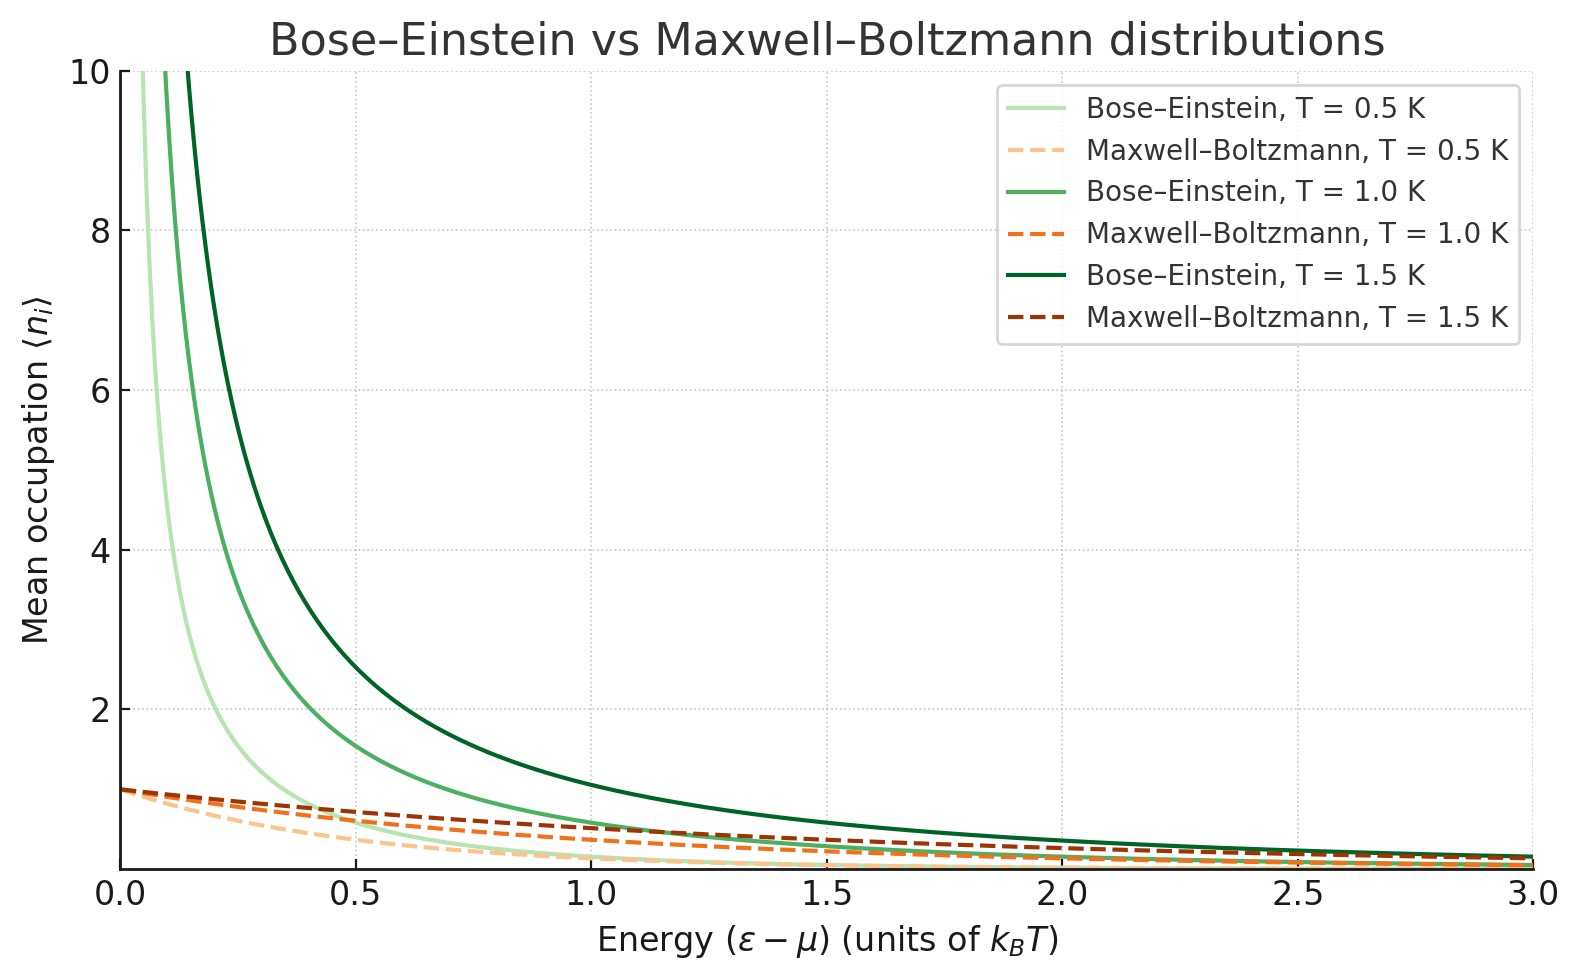
\includegraphics[scale= 0.2]{Chapters/Chapter_2/Images/2_BE_MB.jpg}
    \caption{Comparison between the Bose--Einstein and Maxwell--Boltzmann distributions at different temperatures.}
    \label{Figure 5 - BE_MB}
\end{figure}

\paragraph{Temperature dependence.}
The temperature dependence of the Bose--Einstein distribution is shown in Fig.~\ref{Figure 4 - Bose_Einstein_distribution} and further compared with the Maxwell--Boltzmann distribution at various temperatures in Fig.~\ref{Figure 5 - BE_MB}.
At high temperatures, the distribution is broad and relatively flat, resembling the classical Maxwell--Boltzmann form.  
As the temperature decreases, the distribution becomes increasingly peaked near the lowest energies.
When the critical temperature \( T_c \) is reached, a macroscopic number of particles condense into this state.

\section{Particle Number and Critical Density}

The total number of particles in a Bose gas is obtained by summing the average occupation of all single-particle states:
\begin{equation}
    N = \sum_i \langle n_i \rangle
      = \sum_i \frac{1}{e^{\beta(\varepsilon_i - \mu)} - 1}.
\end{equation}
In the thermodynamic limit\footnote{%
The thermodynamic limit refers to the situation in which the number of particles \(N\) and the volume \(V\) both tend to infinity while their ratio \(n = N/V\) remains constant.  
In this limit, discrete energy levels become quasi-continuous, allowing the replacement of the sum over states by an integral weighted by the density of states \(D(\varepsilon)\).%
}, this sum becomes an integral over the energy spectrum:
\begin{equation}
    N = \int_0^{\infty} D(\varepsilon)\, f(\varepsilon)\, d\varepsilon
      = \int_0^{\infty} \frac{D(\varepsilon)}{e^{\beta(\varepsilon - \mu)} - 1}\, d\varepsilon,
    \label{eq:N_integral}
\end{equation}
where \( f(\varepsilon) \) is the Bose–Einstein distribution and \( D(\varepsilon) \) is the \textit{density of states} (DOS), i.e. the number of single-particle states per unit energy interval.\\
For a three-dimensional gas of nonrelativistic particles confined in a volume \(V\), the quantization of momentum space yields\footnote{For a full derivation of the three-dimensional density of states \(D_{3D}\), see Appendix~\ref{app:BEC-derivation}, Section~\ref{density_of_states}.}:
\begin{equation}
    D_{3D}(\varepsilon) = \frac{V}{4\pi^2}
        \left(\frac{2m}{\hbar^2}\right)^{3/2} \varepsilon^{1/2}.
    \label{eq:DOS_3D}
\end{equation}
Substituting Eq.~\eqref{eq:DOS_3D} into Eq.~\eqref{eq:N_integral} and dividing by \(V\) yields the particle density:
\begin{equation}
\boxed{
    n = \frac{N}{V}
      = A \int_0^{\infty} d\varepsilon\, 
        \frac{\varepsilon^{1/2}}{e^{\beta(\varepsilon - \mu)} - 1},
    }
    \qquad
    A = \frac{m^{3/2}}{\sqrt{2}\pi^2\hbar^3}.
    \label{eq:n_integral_general}
\end{equation}

\subsection*{Critical Density}
To ensure a physically meaningful (non-negative) occupation number,
\[
\langle n_i \rangle = \frac{1}{e^{\beta(\varepsilon_i - \mu)} - 1} > 0,
\]
the denominator must remain positive, implying \( e^{\beta(\varepsilon - \mu)} > 1 \), i.e.\ \( \varepsilon > \mu \).  
In particular, for the lowest energy level (\(\varepsilon = 0\)), this requires
\[
\mu < 0.
\]

As the temperature decreases, \( \mu \) approaches zero from below, indicating that the lowest states become increasingly populated.  
When \( \mu \to 0^- \), a macroscopic occupation of the ground state begins to appear.  
In this limit, the maximum density that can be supported by the excited states is:
\begin{equation}
    n_c = A \int_0^{\infty} d\varepsilon\, 
           \frac{\varepsilon^{1/2}}{e^{\beta \varepsilon} - 1}.
    \label{eq:nc_integral}
\end{equation}

Introducing the dimensionless variable \( x = \varepsilon / (k_B T) \), we have:
\begin{equation}
    n_c = A (k_B T)^{3/2} 
          \int_0^{\infty} dx\, \frac{x^{1/2}}{e^x - 1}.
\end{equation}
The integral can be evaluated using the Gamma and Riemann zeta functions\footnote{For an introduction to and evaluation of this integral using the Gamma and Riemann zeta functions, see Appendix~\ref{app:BEC-derivation}, Section~\ref{appendix:gamma_riemann}.}:
\[
    \int_0^{\infty} \frac{x^{\alpha - 1}}{e^x - 1} dx = \Gamma(\alpha)\, \zeta(\alpha).
\]
For \( \alpha = 3/2 \), we obtain:
\begin{equation}
\boxed{
    n_c  = 
            A (k_B T)^{3/2}
          \,\Gamma\!\left(\tfrac{3}{2}\right)
          \,\zeta\!\left(\tfrac{3}{2}\right) = 
          \frac{m^{3/2}}{\sqrt{2}\pi^2\hbar^3} (k_B T)^{3/2}
          \,\Gamma\!\left(\tfrac{3}{2}\right)
          \,\zeta\!\left(\tfrac{3}{2}\right)
        }
          \label{eq:nc_result}
\end{equation}
It is convenient to introduce the thermal de Broglie wavelength
\begin{equation}
    \lambda_T = \frac{h}{\sqrt{2\pi m k_B T}},
\end{equation}
so that, using $\Gamma(3/2) = \sqrt{\pi}/2$, one finds
\begin{equation}
    n_c = \frac{1}{\lambda_T^3}\,\zeta\!\left(\tfrac{3}{2}\right),
\end{equation}
The quantity \(n_c\) thus represents the \textit{critical density} of particles that can be accommodated in the excited states at temperature \(T\).  
When the total particle density \(n\) exceeds this value, the surplus particles must accumulate in the ground state, giving rise to condensation.  
This formulation also reveals the physical significance of \(\lambda_T\):  
Bose–Einstein condensation occurs when the thermal wavelength becomes comparable to the mean interparticle spacing.

\subsection*{Critical Temperature and Condensate Fraction}
As discussed above, when the total density exceeds the critical value \(n_c\), the excess particles can no longer be accommodated in the excited states and therefore accumulate in the lowest energy level.
The total particle density can thus be expressed as:
\begin{equation}
    n = n_0 + n_{\mathrm{ex}},
    \label{eq:n_total}
\end{equation}
where \( n_0 \) represents the condensate density and \( n_{\mathrm{ex}} \) the density of particles occupying excited states.

\paragraph{Determination of the critical temperature.}
The critical temperature \(T_c\) corresponds to the point at which the density of thermally excited particles equals the total density, i.e.\ \(n = n_{\mathrm{ex}}(T_c) = n_c\).  
Using Eq.~\eqref{eq:nc_result} for \(n_c\) and the explicit form of \(A\) from Eq.~\eqref{eq:n_integral_general}, we have:
\[
n = \frac{m^{3/2}}{\sqrt{2}\pi^2\hbar^3} (k_B T_c)^{3/2}
          \,\Gamma\!\left(\tfrac{3}{2}\right)
          \,\zeta\!\left(\tfrac{3}{2}\right) = 
\frac{m^{3/2}(k_B T_c)^{3/2}}{2\sqrt{2}\,\pi^{3/2}\hbar^3}\,
      \zeta\!\left(\tfrac{3}{2}\right).
\]
Solving for \(T_c\):
\begin{equation}
(k_B T_c)^{3/2} = 
\frac{(2\pi\hbar^2)^{3/2}}{m^{3/2}}
\frac{n}{\zeta(3/2)}
\quad \Longrightarrow \quad
\boxed{
T_c = 
\frac{2\pi\hbar^2}{m k_B}
\left[\frac{n}{\zeta(3/2)}\right]^{2/3}
}\, .
\label{eq:Crit_T}
\end{equation}
This relation defines the transition temperature below which Bose--Einstein condensation occurs.

\paragraph{Derivation of the condensate fraction.}
For \( T < T_c \), the chemical potential remains fixed at \( \mu = 0 \), and the number of particles in excited states is:
\begin{equation}
    N_{\mathrm{ex}}(T) = V A (k_B T)^{3/2}
    \Gamma\!\left(\tfrac{3}{2}\right)
    \zeta\!\left(\tfrac{3}{2}\right),
    \label{eq:Nex_T}
\end{equation}
At \( T = T_c \), the total number of particles is:
\begin{equation}
    N = N_{\mathrm{ex}}(T_c)
      = V A (k_B T_c)^{3/2}
        \Gamma\!\left(\tfrac{3}{2}\right)
        \zeta\!\left(\tfrac{3}{2}\right).
    \label{eq:N_Tc}
\end{equation}
Dividing Eq.~\eqref{eq:Nex_T} by Eq.~\eqref{eq:N_Tc} gives the temperature dependence of the non-condensed fraction:
\[
    \frac{N_{\mathrm{ex}}(T)}{N}
    = \left(\frac{T}{T_c}\right)^{3/2}.
    \label{eq:Nex_fraction}
\]
Since the total number is \( N = N_0 + N_{\mathrm{ex}} \), the condensate population becomes:
\begin{equation}
\boxed{
    \frac{N_0}{N}
    = 1 - \left(\frac{T}{T_c}\right)^{3/2}.
    }
    \label{eq:condensate_fraction}
\end{equation}
This expression shows that the condensate fraction grows continuously from zero at \( T = T_c \) to unity as \( T \to 0 \).


\subsection*{Dimensionality Effects in BEC}
\label{Dimension_BEC}
The occurrence of Bose--Einstein condensation strongly depends on the dimensionality of the system and on the form of the single-particle dispersion relation.  
To illustrate this, we generalize the derivation of the critical density to lower dimensions and show explicitly that condensation cannot occur in two or one dimensions for nonrelativistic particles with quadratic dispersion.

\paragraph{Two-dimensional case.}
For a gas of nonrelativistic bosons confined in a square box of side \(L\), the single-particle energy levels are given by:
\[
    \varepsilon = \frac{\hbar^2}{2m}(k_x^2 + k_y^2),
\]
where: 
\[
k_x = \frac{\pi n_x}{L}, \qquad 
k_y = \frac{\pi n_y}{L}, \qquad 
n_x, n_y \in \mathbb{Z}.
\]
The density of states follows from counting the number of states within a ring of radius \(k\) and thickness \(dk\) in \(k\)-space.  
Each quantum state occupies an area \((2\pi/L)^2\), so the number of states between \(k\) and \(k+dk\) is: 
\[
  dN = \frac{L^2}{(2\pi)^2} \, 2\pi k\, dk  
\]
Since the particle energy is related to the wavevector by 
\(\varepsilon = \hbar^2 k^2 / (2m)\), we have: 
\[
    k\, dk = (m/\hbar^2)\, d\varepsilon \implies dN = \frac{L^2 m}{2\pi \hbar^2}\, d\varepsilon \implies 
D_{2\mathrm{D}}(\varepsilon) = \frac{dN}{d\varepsilon}
= \frac{mL^2}{2\pi \hbar^2}.
%\label{eq:DOS_2D}
\]
Unlike the three-dimensional case, the DOS is \textit{independent of energy}.  
The total number of particles occupying excited states is therefore:
\[
    N_{2\mathrm{D}} = \int_0^{\infty} 
    \frac{D_{2\mathrm{D}}\, d\varepsilon}
         {e^{\beta(\varepsilon - \mu)} - 1}
    = \frac{mL^2}{2\pi \hbar^2}
      \int_0^{\infty}
      \frac{d\varepsilon}{e^{\beta(\varepsilon - \mu)} - 1}.
    %\label{eq:N2D_integral}
\]
Expanding the Bose--Einstein factor using the geometric series
\[\frac{1}{e^{\beta(\varepsilon - \mu)} - 1} 
= \frac{e^{-\beta(\varepsilon - \mu)}}{1 - e^{-\beta(\varepsilon - \mu)}}
\]
and introducing the fugacity\footnote{The fugacity \( z = e^{\beta \mu} \) quantifies the effect of the chemical potential on the particle distribution.  
It measures the deviation of the system from the classical limit, where \( z \ll 1 \) corresponds to low densities (Maxwell--Boltzmann regime) and \( z \to 1^{-} \) signals the onset of quantum degeneracy.} \( z = e^{\beta \mu} \), we can express the integrand as
\[
    \frac{1}{e^{\beta(\varepsilon - \mu)} - 1}
    = \sum_{l=1}^{\infty} e^{-l\beta(\varepsilon - \mu)}
    = \sum_{l=1}^{\infty} z^l e^{-l\beta\varepsilon}.
\]
Substituting this expansion into the integral and integrating over the energy gives:
\[
    \int_0^{\infty} e^{-l\beta\varepsilon}\, d\varepsilon = \frac{1}{l\beta},
\]
which leads to:
\[
    N_{2\mathrm{D}} = 
    \frac{mL^2}{2\pi \hbar^2 \beta}
    \sum_{l=1}^{\infty} \frac{z^l}{l}.
\]
This summation represents a particular case of the \textit{Bose function}, defined in general\footnote{%
It appears frequently in the statistical description of Bose gases and reduces to the 
Riemann zeta function at the condensation point, $g_{\sigma}(1) = \zeta(\sigma).$  
} as
\begin{equation}
    g_{\sigma}(z) = \sum_{l=1}^{\infty} \frac{z^l}{l^{\sigma}},
    \qquad (|z|<1),
\end{equation}
In the present case, \(\sigma = 1\), the series can be summed in closed form using the identity:
\[
    \sum_{l=1}^{\infty} \frac{z^l}{l} = -\ln(1-z)\qquad (|z|<1).
\]
Therefore:
\[
    N_{2\mathrm{D}} 
    = \frac{mL^2}{2\pi \hbar^2 \beta}
      \sum_{l=1}^{\infty} \frac{z^l}{l}
    = -\frac{mL^2}{2\pi \hbar^2 \beta}\, \ln(1 - z).
\]
As the chemical potential approaches zero (\(\mu \to 0^{-}\), i.e.\ \(z=e^{\beta\mu}\to 1^{-}\)), the series diverges logarithmically. Hence the excited–state population:
\begin{equation}
    N_{2\mathrm{D}} = -\frac{mL^2}{2\pi \hbar^2 \beta}\,\ln(1-z)
\end{equation}
blows up. This logarithmic divergence indicates that long-range coherence cannot develop in a two-dimensional gas at any finite temperature. Thus, for massive bosons with quadratic dispersion in two dimensions,
\[
    \textit{BEC does not occur at any finite temperature \;} T.
\]

 This limitation becomes even more severe in one dimension, where the density of states further enhances the divergence.

\paragraph{One-dimensional case.}
In one dimension, the single-particle energy is:
\[
    \varepsilon = \frac{\hbar^2 k^2}{2m},
\]
and the number of states between \(k\) and \(k + dk\) in a box of length \(L\) is:
\[
    dN = \frac{L}{\pi} dk.
\]
Hence the density of states is:
\begin{equation}
    D_{1\mathrm{D}}(\varepsilon)
    = \frac{dN}{d\varepsilon}
    = \frac{L}{\pi \hbar} \sqrt{\frac{m}{2\varepsilon}}.
    \label{eq:DOS_1D}
\end{equation}
The total number of particles in excited states becomes:
\begin{equation}
    N_{1\mathrm{D}} = 
    \int_0^{\infty}
    \frac{D_{1\mathrm{D}}(\varepsilon)\, d\varepsilon}
         {e^{\beta(\varepsilon - \mu)} - 1}
    = \frac{L}{\pi \hbar} \sqrt{\frac{m}{2}}
      \int_0^{\infty}
      \frac{\varepsilon^{-1/2}\, d\varepsilon}
           {e^{\beta(\varepsilon - \mu)} - 1}.
\end{equation}
In the limit \(\mu \to 0\), the integrand behaves as \(\varepsilon^{-1/2}\) near \(\varepsilon = 0\), which causes the integral to diverge.  
As in the 2D case, all particles can be accommodated in excited states, and no condensation occurs at any finite temperature.

\paragraph{Dimensional Criterion for BEC.}\label{crit}
The absence of Bose--Einstein condensation in one and two dimensions reflects the dominance of low-energy fluctuations in reduced dimensionality.\\
For a dispersion relation of the form \(\varepsilon \propto K^s\), one can show that condensation occurs only if the integral
\begin{equation}
    \int_0^{\infty} \frac{\varepsilon^{d/s - 1}\, d\varepsilon}{e^{\beta(\varepsilon - \mu)} - 1}
    \label{convergence}
\end{equation}
converges when \(\mu \to 0\), which requires \(d/s > 1\).  
For quadratic dispersion $(s = 2)$, this condition is satisfied only for $d > 2$.
Therefore, true Bose–Einstein condensation is possible only in three or more dimensions.
In lower dimensions, quantum degeneracy effects can still appear, but they manifest as quasi-condensation rather than macroscopic occupation of a single quantum state.

The appearance of the condensate below the critical temperature $T_c$ signifies more than a simple redistribution of particles among energy levels.
It marks the emergence of a collective quantum state in which a macroscopic number of particles share the same single-particle wavefunction.
This coherence allows the entire system to be described by a single complex field, the \textit{macroscopic wavefunction} or \textit{order parameter}, whose magnitude reflects the condensate density and whose phase encodes its quantum coherence.\\
The Bose–Einstein condensation transition can thus be interpreted as a spontaneous breaking of the global $\mathrm{U}(1)$ phase symmetry associated with particle number conservation, a concept that will prove central in the description of superconductivity.\\
We now formalize this idea.

\section{Order Parameter and SSB}
We now formalize this idea by introducing the concept of the \textit{order parameter}, which characterizes the macroscopic coherence of the Bose–Einstein condensate.
Rather than describing the gas in terms of individual particle states, we can instead represent it through a single collective field that embodies both the amplitude and phase of the condensate.

\subsection*{Order Parameter}  
Below the critical temperature \(T_c\), a macroscopic number of particles occupy the same single-particle state \(\chi_0(\mathbf{r},t)\).  
The system can therefore be described by a collective complex field, the \textit{macroscopic wavefunction} or \textit{order parameter}:
\[
    \Psi(\mathbf{r},t) = \sqrt{N_0(t)}\, \chi_0(\mathbf{r},t),
    %\label{eq:order_parameter_def}
\]
where \(N_0(t)\) is the number of particles in the condensate.  
Since the single-particle wavefunction is normalized to unity, the normalization of \(\Psi\) satisfies
\[
    \int |\Psi(\mathbf{r},t)|^2\, d\mathbf{r} = N_0(t).
\]
The modulus \(|\Psi(\mathbf{r},t)|^2\) thus represents the local condensate density, while its phase encodes the global coherence of the quantum state.  \\
Conversely, above $T_c$, the phases of the individual particle states are random and uncorrelated, and the average macroscopic field vanishes, \(\Psi = 0\).

The order parameter therefore serves as a direct indicator of the phase transition:
\[
    \Psi(\mathbf{r},t) =
    \begin{cases}
        0, & T \geq T_c,\\[4pt]
        \neq 0, & T < T_c.
    \end{cases}
\]

A finite amplitude of $\Psi$ below $T_c$ signals the emergence of long-range coherence throughout the system, marking the onset of Bose–Einstein condensation.

\subsection*{Spontaneous Breaking of \texorpdfstring{$\mathrm{U}(1)$}{U(1)} Symmetry}

As discussed before, the formation of a Bose--Einstein condensate introduces a nonzero complex order parameter
\[
\Psi = \sqrt{n_0}\, e^{i\phi},
\]
whose modulus sets the condensate density and whose phase \(\phi\) defines its global coherence.  
While the phase itself has no direct influence on measurable quantities such as the density \(|\Psi|^2\), the act of choosing a definite value of \(\phi\) has deep physical significance: it marks the spontaneous breaking of a continuous symmetry.\\
Above the critical temperature \(T_c\), the gas has no preferred phase.  
Each particle’s wavefunction carries a random phase, and the macroscopic average vanishes, \(\Psi = 0\).  
In this regime, the system is invariant under global phase transformations,
\[
\Psi \;\to\; e^{i\theta}\Psi,
\]
so all phases are physically equivalent.\\
Below \(T_c\), however, a macroscopic number of particles condense into the same quantum state, and the order parameter acquires a finite value.  
Although the microscopic equations remain symmetric under the same phase rotations, the condensate itself must \emph{select} one specific phase \(\phi\) to establish coherence.  
The symmetry of the underlying laws is therefore preserved, but the symmetry of the macroscopic state is not, which is the essence of \textit{spontaneous symmetry breaking} (SSB).

The broken \(\mathrm{U}(1)\) phase symmetry introduces a new physical quantity, the global phase of the condensate, common to all particles and uniform throughout the system.  \\
Hence, Bose--Einstein condensation can be seen not only as the macroscopic occupation of the ground state, but as the spontaneous emergence of global phase order, a fundamental concept that will reappear in the description of superconductivity.

%==========================================================================



\chapter{Superconductivity as a BEC of Pairs}
In chapter \ref{Ch_2} we have shown that superconductivity originates from the pairing of electrons into correlated states known as \textit{Cooper pairs}.  
Each pair carries charge \(2e\) and total spin zero\footnote{In the singlet case: two electrons with opposite spins $(\uparrow\downarrow)$ combine to give a total spin $J = 0$.} and thus behaves as a composite boson.  
When cooled below a critical temperature \(T_c\), these composite bosons condense into a single macroscopic quantum state characterized by long-range phase coherence.  
This condensed state constitutes the superconducting phase.

\section{Macroscopic Analogy}
From a macroscopic standpoint, superconductivity and Bose--Einstein condensation share the same fundamental feature: both arise from the occupation of a single quantum state by a macroscopic number of particles.  
The key distinction lies in the microscopic mechanism that forms the condensed particles:  

\begin{itemize}
    \item \textbf{Bose--Einstein condensate:} In a conventional Bose gas, the constituent particles are \emph{elementary bosons} (e.g.\ atoms or photons) that condense directly into the lowest energy state below a critical temperature.

    \item \textbf{Superconductor:} In a superconductor, the condensed entities are not elementary particles but \emph{composite bosons} (bound states of two electrons known as \emph{Cooper pairs}), each carrying charge \(2e\) and integer spin.
    The condensation of these composite bosons into a single coherent quantum state produces the superconducting phase.
\end{itemize}

Hence, superconductivity can be viewed as a \textit{Bose--Einstein condensation of Cooper pairs}.

The analogy is made even clearer through the order parameter formalism.  
In BEC, the macroscopic wavefunction of the condensate is expressed as 
\[
\Psi(\mathbf{r}) = \sqrt{n_0(\mathbf{r})}\, e^{i\phi(\mathbf{r})},
\]
where \(n_0\) is the condensate density and \(\phi\) its global phase.  
In a superconductor, the order parameter takes an analogous form,
\[
\Delta = |\Delta| e^{i\phi},
\]
whose magnitude \(|\Delta|\) measures the superconducting energy gap, and whose phase \(\phi\) defines the macroscopic coherence of the condensate.  
Below the critical temperature \(T_c\), \(\Delta\) acquires a finite value, signalling the onset of long-range phase order and the spontaneous breaking of the global \(\mathrm{U}(1)\) gauge symmetry.  
This broken symmetry gives rise to the collective quantum state responsible for superconductivity.

Hence, while the mechanisms of pairing and condensation differ, their consequence is the same: a \textit{phase-coherent macroscopic quantum state}.  \\
This correspondence naturally raises a question:
\begin{center}
\textit{Do the BCS and BEC descriptions represent two distinct phases, or merely two limits of a single underlying phenomenon?}
\end{center}

%\section{Weak- To Strong- Coupling Regime} %TO DO!! Choose one
\section{The BCS-BEC Crossover}

A unified description of superconductivity can be obtained by extending the Bose--Einstein condensation formalism to include systems of composite bosons whose dispersion relation depends on the strength of the underlying fermionic attraction. 

\subsection*{General expression for the critical temperature.}
The condensation temperature and the dimensionality dependence can be derived for a general dispersion relation of the form
\[
    \varepsilon_K = C_s K^s,
\]
where \(C_s\) is a dimensional constant and \(s\) defines how the excitation energy scales with momentum. For a $d$-dimensional system the critical temperature reads:
\begin{equation}
\boxed{
    T_c = \frac{C_s}{k_B}
    \left[
        \frac{s\, \Gamma(d/2)\, (2\pi)^d\, n_B}
             {2\, \pi^{d/2}\, \Gamma(d/s)\, g_{d/s}(1)}
    \right]^{s/d}}\, ,
    \label{eq:Tc_general_1}
\end{equation}
where \(n_B\) is the boson (or Cooper-pair) density and we recall $g_{d/s}$ is the Bose function of order $d/s$. Using the relation,
\[
g_{\sigma}(1) = \zeta(\sigma) \iff g_{d/s}(1) = \zeta(d/s) 
\]
\eqref{eq:Tc_general_1} can be equivalently written as:
\begin{equation}
\boxed{
    T_c = \frac{C_s}{k_B}
    \left[
        \frac{s\, \Gamma(d/2)\, (2\pi)^d\, n_B}
             {2\, \pi^{d/2}\, \Gamma(d/s)\, \zeta(d/s)}
    \right]^{s/d}}\, ,
    \label{eq:Tc_general_2}
\end{equation}

The condensation condition requires \(d/s > 1\), ensuring that the number integral converges [Eq.~\eqref{convergence}]. For the conventional case of quadratic dispersion, condensation is possible only if \(d > 2\), as we have already seen in section \ref{crit}. Hence, in strictly two-dimensional systems, the integral diverges and no finite critical temperature can exist.\\
Then, 
\begin{center}
    \textit{How can we observe superconductivity, or equivalently, Bose--Einstein condensation of pairs, in two-dimensional materials?}
\end{center}
The answer lies in the nature of the pair dispersion relation.  
In presence of a Fermi sea, the Pauli exclusion principle restricts the available momentum states for pairing, causing the centre-of-mass motion of the pairs to deviate from the free-particle quadratic law.  
As a result, the pair dispersion becomes approximately \emph{linear} rather than quadratic: this modification is directly linked to the strength of the underlying attractive interaction between fermions, which determines whether the system behaves in the weak- or strong-coupling limit.

\subsection*{Weak-coupling regime: BCS Limit}

In the weak-coupling limit, the attractive interaction between fermions is small compared to the Fermi energy, a condition quantified by the dimensionless ratio
\[
\frac{E_b}{\varepsilon_F} \ll 1,
\]
where \(E_b\) denotes the pair binding energy and \(\varepsilon_F\) the Fermi energy.  
In this regime, the binding energy of a Cooper pair is much smaller than the characteristic energy scale of the Fermi sea.  
The pairs are therefore highly delocalized in real space, with sizes much larger than the average interparticle distance, and they overlap extensively with one another.  
Because of this strong overlap, pair formation and condensation occur simultaneously at the same temperature \(T_c\), a defining feature of the \textit{BCS limit}:
\[
T_{\text{pair formation}} = 
T_{\text{condensation}} = T_c
\]

Microscopically, Cooper pairs form within the filled Fermi sea.  
However, the Pauli exclusion principle forbids the constituent fermions from occupying states already filled below the Fermi surface, restricting the available momentum states for pairing.  
This exclusion modifies the pair’s centre-of-mass motion: instead of moving freely as in vacuum, the pair interacts with the background Fermi sea.  
Consequently, its energy no longer follows the free-particle quadratic dependence on momentum but becomes approximately \textit{linear}:
\begin{equation}
    \varepsilon_K \approx \alpha(d)\, \hbar v_F\, K,
    \label{eq:linear_dispersion}
\end{equation}
where \(v_F\) is the Fermi velocity and \(\alpha(d)\) is a dimension-dependent coefficient, which values are \(\alpha(2) = 2/\pi\), \(\alpha(3) = 1/2\).  
This linear dispersion reflects the coupling of the pair’s motion to collective excitations near the Fermi surface and is a direct consequence of Pauli blocking.

Substituting \(s = 1\), $C_1 = \alpha(d)\, \hbar v_F$ into the generalized critical temperature formula~\eqref{eq:Tc_general_1}, we obtain another special case\footnote{For the full derivation, see Appendix \ref{app:BCS_BEC-derivation}, section \ref{app:Tc_linear_dispersion}.}:
\begin{equation}
\boxed{
    T_c = \frac{\alpha(d)\,\hbar v_F}{k_B}
    \left[
        \frac{\pi^{(d+1)/2}\, n_B}
             {\Gamma\!\left[(d+1)/2\right]\, g_d(1)}
    \right]^{1/d}}\,.
    \label{eq:Tc_linear_dispersion}
\end{equation}
This expression shows that for linear dispersion, the condensation temperature \(T_c\) remains finite for all \(d > 1\), thereby resolving the apparent paradox of superconductivity in quasi-two-dimensional systems.

\paragraph{Pair Breakup and the Finite Critical Temperature}
The previous analysis assumes the existence of ``unbreakable'' Cooper pairs, i.e.\ bound states that persist for all centre-of-mass momenta (CMM) from \(K = 0\) to \(K \to \infty\).  
In this idealized case, the integration over all momenta in the number equation leads to the result~\eqref{eq:Tc_linear_dispersion} for the condensation temperature.  
However, in a more realistic scenario, Cooper pairs can dissociate into two unpaired fermions once their total momentum exceeds a finite value \(K_0\).  
This critical momentum corresponds to the point where the pair binding energy vanishes,
\[
\Delta_{K_0} = 0,
\]
and defines the upper limit for the existence of stable pairs.

The breakup momentum \(K_0\) increases with the coupling strength:  
in the weak-coupling limit it is approximately
\[
K_0 \simeq \frac{\Delta_0}{a(d)\,\hbar v_F},
\]
and tends to infinity as the coupling becomes very strong (\(\Delta_0 \to \infty\)).  
Physically, \(K_0\) represents the maximum centre-of-mass momentum that a Cooper pair can sustain before dissociating into unpaired fermions.

By replacing the upper integration limit in the number equation with \(K_0\),  
the total boson number can be expressed in its general \(d\)-dimensional form as
\begin{equation}
N_{d\mathrm{D}} 
= \int_0^{\varepsilon_{K_0}} D_{d\mathrm{D}}(\varepsilon)\, f(\varepsilon)\, d\varepsilon
= \int_{|\mathbf K|\le K_0}\!\frac{d^d K}{(2\pi)^d}\, f(\varepsilon_K)
= \int_{|\mathbf K|\le K_0}\!\frac{d^d K}{(2\pi)^d}\,
      \frac{1}{e^{\beta(\varepsilon_K-\mu)} - 1}.
\end{equation}

From this modified number equation, it's possible to derive the asymptotic behaviour of the critical temperature in the limit of vanishing pair binding energy (\(\Delta_0 \to 0\)):
\begin{equation}
\boxed{
T_c \simeq
\frac{(d-1)\,[2\pi a(d)\hbar v_F]^d\, n_B}
{A_d\, k_B\, \Delta_0^{\,d-1}}
\quad \xrightarrow[\Delta_0 \to 0]{} \infty}\, ,
\label{eq:Tc_divergent}
\end{equation}
where \(A_2 = 2\pi\) and \(A_3 = 4\pi/3\).

Equation~\eqref{eq:Tc_divergent} shows that, as the pair binding energy \(\Delta_0\) approaches zero, the predicted critical temperature diverges.  
This unphysical result arises because, in this limit, all remaining pairs occupy the \(K = 0\) state at any temperature, implying that the system would be condensed at all \(T\).  
Physically, this corresponds to a situation in which the pair breakup threshold disappears, and every pair remains bound regardless of thermal excitation.

In practice, however, Cooper pairs do not remain bound for arbitrarily large centre-of-mass momenta.
Above a finite threshold $K_0$ the attractive interaction is no longer strong enough to keep the electrons paired, and the pair breaks apart into two unbound fermions.\\
When this physically unavoidable pair-breaking process happens, resulting in a more realistic \textit{binary boson–fermion mixture}, the artificial divergence of $T_c$ disappears.
The available phase space for bosonic excitations becomes finite, and the critical temperature is “regularized’’ to a finite value. Remarkably, this corrected $T_c$ turns out to be very close to the one predicted by the ideal Bose gas expression~\eqref{eq:Tc_linear_dispersion}, confirming that the divergence arose solely from the unphysical assumption of unbreakable pairs extending to infinite momentum.

\subsection*{Strong-coupling regime: BEC Limit}
In the strong-coupling limit, the attractive interaction between fermions dominates over the Fermi energy, a condition expressed by
\[
\frac{E_b}{\varepsilon_F} \gg 1.
\]
Here, the pair binding energy \(E_b\) is much larger than the characteristic energy scale of the Fermi sea.  
As a result, electrons form tightly bound pairs even in the absence of a Fermi surface, and these pairs behave as compact composite bosons.  
Their spatial size becomes much smaller than the average interparticle spacing, and the overlap between different pairs is negligible.  
Pair formation and condensation therefore occur as two distinct processes: pairs form at a higher temperature and subsequently undergo Bose--Einstein condensation into the lowest-energy state at a lower temperature \(T_c\).  
This behaviour can be schematically represented as:
\[
\begin{cases}
\textbf{High temperature: } T > T^{\ast} &
\Rightarrow \text{no bound pairs},\quad \Delta_0 = 0,\; n_B = 0, \\[6pt]
\textbf{Preformed pairs: } T_c < T < T^{\ast} &
\Rightarrow \text{bound pairs w/o coherence},\quad \Delta_0 > 0,\; n_0 = 0,\; \mu < 0, \\[6pt]
\textbf{Condensed phase: } T \leq T_c &
\Rightarrow \text{BEC of pairs},\quad \Delta_0 > 0,\; n_0 > 0,\; \mu < 0.
\end{cases}
\]

where \(T^{\ast}\) denotes the \textit{pairing temperature} at which bound states first appear, 
\(T_c\) is the \textit{condensation temperature}, 
\(\Delta_0\) the pair binding energy at zero momentum, 
\(n_B\) the total pair density, and \(n_0\) the condensate density.

In this regime, the centre-of-mass motion of each pair is no longer influenced by Pauli blocking, since the constituent fermions occupy bound molecular states well below the Fermi level.  
The excitation energy of a pair thus follows the free-particle, \textit{quadratic} dispersion characteristic of a boson with total mass \(2m\):
\[
    \varepsilon_K = \frac{\hbar^2 K^2}{2(2m)}.
    \label{eq:quadratic_dispersion}
\]
The chemical potential becomes negative (\(\mu < 0\)), lying below the bottom of the conduction band, as expected for a gas of bound molecules. 

Substituting \(s = 2\) and \(C_2 = \hbar^2 / (2M)\), with $M = 2m$, into the generalized expression~\eqref{eq:Tc_general_1} yields\footnote{% 
For the full derivation, see Appendix \ref{app:BCS_BEC-derivation}, section \ref{d3s2}.
} the standard result for a three-dimensional Bose gas:
\begin{equation}
    T_c = \frac{2\pi \hbar^2}{M k_B}
          \left[\frac{n_B}{\zeta(3/2)}\right]^{2/3}.
    \label{eq:Tc_strong_coupling}
\end{equation}

This quadratic dispersion corresponds to the \textit{BEC limit} of superconductivity, where tightly bound, localized pairs behave as independent bosons that condense into a single macroscopic quantum state.  



\bigskip
\bigskip
\noindent
In the previous chapters, we have developed a microscopic description of superconductivity: we explained how Cooper pairs form, how superconductivity can be viewed as a Bose--Einstein condensation of pairs, and how the system spans the weak (BCS) and strong (BEC) coupling limits.  \\
We now turn to the \emph{macroscopic} consequences of this condensate, \textit{i.e.} how a complex order parameter varies in space, how it couples to electromagnetic fields, and how measurable responses such as currents, magnetization, and characteristic length scales emerge.  
To explore these large-scale behaviours, we introduce the Landau--Ginzburg theory, a phenomenological approach that links the quantum condensate to the observable properties of real superconductors.









\chapter{Landau-Ginzburg Formalism}%TO DO!! fix the title

\noindent
The previous chapters developed the microscopic foundations of superconductivity: 
from the condensation of bosons in Bose--Einstein statistics to the pairing mechanism that gives rise to the Bardeen--Cooper--Schrieffer state. \\ 
We now turn to a complementary, macroscopic description capable of capturing the large-scale behaviour of superconductors without resolving their microscopic details.  
This is provided by the \emph{Landau--Ginzburg (LG) theory}, a phenomenological framework that expresses superconductivity through a complex order parameter~$\psi(\mathbf{r})$, interpreted as the macroscopic wavefunction of the condensate. Within this theory, spatial variations of~$\psi$ and electromagnetic fields are coupled through a free-energy functional, from which one derives the celebrated \emph{Ginzburg--Landau equations}. 

\section{Landau’s Theory of Phase Transitions}
\label{sec:landau_theory}

The thermodynamic classification of phase transitions introduced by \textit{Ehrenfest} distinguished first-- and second--order transitions according to discontinuities in the derivatives of the free energy.  
Although useful, this description was purely macroscopic and did not address the microscopic origin of the transition itself.  
\textit{Lev Landau} provided a deeper and more general description by linking second--order phase transitions to changes in the \textit{symmetry} of the physical system.

\subsection*{Spontaneous Symmetry Breaking in Ferromagnets}
To illustrate Landau’s reasoning, consider the case of a ferromagnet, whose behaviour is shown schematically in Fig.~\ref{Figure 6 - Ferro_vs_Para}.\\
At high temperatures $(T > T_c)$, the system is in the \emph{paramagnetic} phase: the atomic magnetic moments are randomly oriented due to thermal agitation, and the material as a whole exhibits no net magnetization. This corresponds to the \emph{high-symmetry} phase, where rotational symmetry is preserved.\\
As the temperature decreases below the Curie temperature $T_c$, the magnetic moments spontaneously align, giving rise to a finite magnetization M. The system thus selects a preferred direction in space, breaking the original rotational symmetry.\\
It is this spontaneous symmetry breaking, rather than a discontinuity in thermodynamic quantities, that, according to Landau, captures the true nature of a phase transition.

\begin{figure}[H]
    \centering
    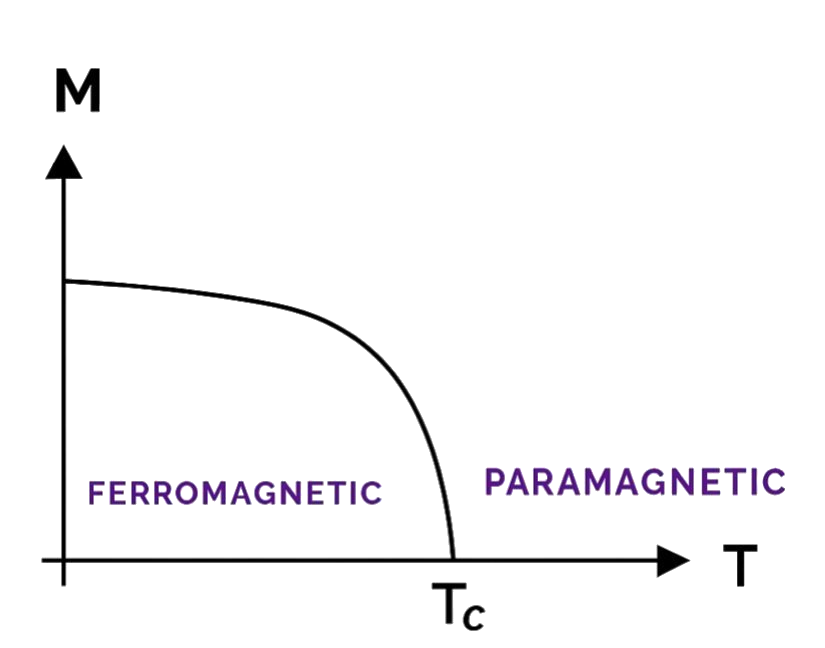
\includegraphics[scale= 0.5]{Chapters/Chapter_5/Images/6_ferromag2.png}
    \caption{Temperature dependence of the magnetization M in a ferromagnet.}
    \label{Figure 6 - Ferro_vs_Para}
\end{figure}

\subsection*{Free-Energy Expansion}
Landau’s key insight was that near the transition point, the state of the system can be described by an order parameter~$\eta$, which measures the degree of symmetry breaking.

\paragraph{The order parameter.}
The order parameter, denoted by \(\eta\), measures the degree of order in the system and distinguishes the two phases:
\[
\eta =
\begin{cases}
0, & T \geq T_c \quad \text{(symmetric phase)},\\[4pt]
\neq 0, & T < T_c \quad \text{(symmetry--broken phase)}.
\end{cases}
\]
For a ferromagnet, \(\eta\) corresponds to the magnetization \(M\); for a superconductor, it will later be identified with the complex condensate wavefunction \(\Psi(\mathbf{r})\).  
As the temperature crosses \(T_c\), the order parameter increases smoothly from zero to a finite value, signaling a continuous (second-order) phase transition.

\paragraph{Free-Energy Functional.}
The central assumption is that the \textit{free energy density} \(f\) of the system can be expanded as a power series in the order parameter \(\eta\), which is small near \(T_c\):
\begin{equation}
    f(T, \eta) = f_n(T) + a(T)\eta^2 + \frac{b(T)}{2}\eta^4 + \dots,
    \label{eq:landau_free_energy}
\end{equation}
where \(f_n(T)\) is the free energy of the normal (symmetric) phase and \(a(T)\), \(b(T)\) are phenomenological coefficients.  
The absence of odd powers in \(\eta\) reflects the assumption of symmetry between the two directions of the order parameter (\(\eta \leftrightarrow -\eta\)).  
The quartic term ensures stability since \(b(T) > 0\).

\paragraph{Equilibrium and Phase Behaviour.}
The equilibrium value of \(\eta\) minimizes the free energy:
\[
\frac{\partial f}{\partial \eta} = 0
\;\Rightarrow\;
2a(T)\eta + 2b(T)\eta^3 = 0.
\]
This yields two possible solutions:
\[
\eta = 0, \qquad \text{or} \qquad \eta^2 = -\frac{a(T)}{b(T)}.
\]
The first solution corresponds to the symmetric phase, the second to the symmetry--broken one.  
To determine which is stable, we examine the sign of \(a(T)\).  
Landau assumed that \(a(T)\) varies linearly near the critical temperature:
\[
a(T) = a_0 (T - T_c), \qquad a_0 > 0.
\]

Now:

\begin{itemize}
    \item For \(T > T_c\), the coefficient \(a(T) \) is positive. Then \(a(T)/b(T) > 0\), so the second solution \(\eta^2 = -a/b\) would be negative, i.e.\ unphysical (since \(|\eta|^2\) cannot be negative).  
    Hence, the only possible solution is
    \[
    \eta = 0.
    \]
    This means that the system minimizes its free energy when there is no order, the symmetric (normal) phase.

    \item For \(T < T_c\), the coefficient \(a(T) < 0\) is negative. Now \(-a/b > 0\), so the solution
    \[
    |\eta| = \sqrt{-\frac{a(T)}{b(T)}}
    \]
    is real and positive.  
    This implies that the free energy is minimized not at \(\eta = 0\), but at some finite value of \(|\eta|\).  
    The system spontaneously chooses one of the equivalent minima (e.g.\ \(+\eta\) or \(-\eta\)), thereby breaking the symmetry.
\end{itemize}

\begin{figure}[H]
    \centering
    %----------------------------------------
    % Panel 1: T > Tc (Single Minimum)
    %----------------------------------------
    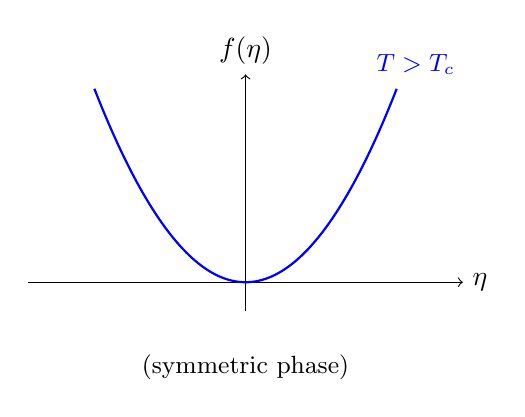
\begin{tikzpicture}[scale=1.2]
        % Axes
        \draw[->] (-2.3,0) -- (2.3,0) node[right] {$\eta$};
        \draw[->] (0,-0.3) -- (0,2.2) node[above] {$f(\eta)$};

        % Free energy curve: single well
        \draw[thick,blue,domain=-1.6:1.6,samples=100] 
            plot(\x,{0.8*\x*\x });
        
        % Label
        \node[above,blue] at (1.8,2.1) {\small $T > T_c$};
        \node at (0,-0.9) {\small (symmetric phase)};
    \end{tikzpicture}
    \hspace{1.5cm}
    %----------------------------------------
    % Panel 2: T < Tc (Double Well)
    %----------------------------------------
    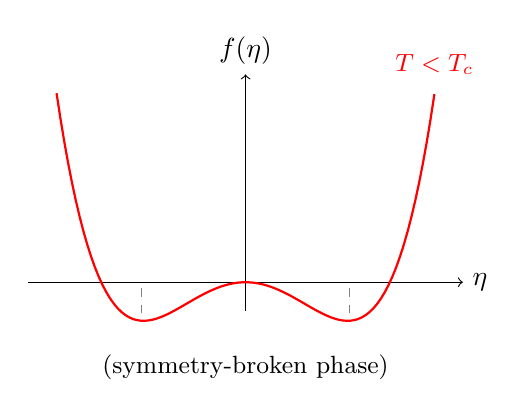
\begin{tikzpicture}[scale=1.2]
        % Axes
        \draw[->] (-2.3,0) -- (2.3,0) node[right] {$\eta$};
        \draw[->] (0,-0.3) -- (0,2.2) node[above] {$f(\eta)$};

        % Free energy curve: double well
        \draw[thick,red,domain=-2:2,samples=100] 
            plot(\x,{0.3*\x*\x*\x*\x - 0.7*\x*\x});

        % Dashed lines at minima
        \draw[dashed,gray] (-1.1,-0.33) -- (-1.1,0);
        \draw[dashed,gray] (1.1,-0.33) -- (1.1,0);
        %\node[below] at (-1.2,0.7) {\small $-\!|\eta|$};
        %\node[below] at (1,0.7) {\small $+|\eta|$};
        
        % Label
        \node[above,red] at (2,2.1) {\small $T < T_c$};
        \node at (0,-0.9) {\small (symmetry-broken phase)};
    \end{tikzpicture}

    %----------------------------------------
    % Caption
    %----------------------------------------
    \caption{
    Landau free energy $f(\eta)$ above and below the critical temperature $T_c$.  
    For $T > T_c$ (left), the free energy has a single minimum at $\eta = 0$, corresponding to the symmetric, normal phase.  
    For $T < T_c$ (right), $a(T)$ becomes negative and $f(\eta)$ develops two degenerate minima at $\pm|\eta|$, indicating spontaneous symmetry breaking and the emergence of long-range order.
    }
    \label{fig:landau_free_energy_panels}
\end{figure}

In the next section, we apply this phenomenological expansion to superconductivity by identifying the order parameter \(\eta\) with the complex macroscopic wavefunction \(\Psi(\mathbf{r})\), which represents the superconducting condensate.


\section{The Ginzburg--Landau Free Energy Functional}
\label{sec:GL-functional}

Having established Landau’s general framework for second-order phase transitions, 
we now apply the same reasoning to superconductivity.\\
In this context, the order parameter is the complex macroscopic wavefunction
\[
\Psi(\mathbf{r}) = |\Psi(\mathbf{r})| e^{i\phi(\mathbf{r})},
\]
which represents the collective quantum state of the superconducting condensate.\\
Following the Landau approach, the free energy of the superconducting phase is expanded in powers of the small quantity $|\Psi|$ near the critical temperature.

\subsection*{Free energy in the uniform case} 
Consider first a uniform superconductor in absence of external magnetic fields.  
Let $F_s(T,V)$ and $F_n(T,V)$ denote the free energies of the superconducting and normal states, respectively.\footnote{%
We use the \emph{free energy} rather than the internal energy because it depends naturally on temperature and is therefore suited for studying thermal phase transitions near $T_c$.}
Since the two phases differ just slightly close to $T_c$, the free energy of the superconducting phase can be written as
\begin{equation}
F_s(T,V) = F_n(T,V) + V\!\left[a(T)|\Psi|^2 + \frac{b(T)}{2}|\Psi|^4 + \dots\right],
\label{eq:GL_free_energy_uniform}
\end{equation}
where $a(T)$ and $b(T)$ are phenomenological coefficients, with $b(T) > 0$ ensuring stability. This is precisely the same form as the Landau expansion \eqref{eq:landau_free_energy}, now generalized to a complex order parameter.\\
The equilibrium value of $|\Psi|$ minimizes $F_s$.  
Neglecting higher-order terms, the condition $\partial F_s / \partial |\Psi| = 0$ gives
\[
|\Psi|^2 = 
\begin{cases}
0, & T > T_c,\\[4pt]
-\dfrac{a(T)}{b(T)}, & T < T_c,
\end{cases}
\qquad \text{with } a(T) = a_0(T - T_c), \ a_0 > 0.
\]
Thus, for $T > T_c$, the minimum occurs at $|\Psi| = 0$ (normal phase), 
whereas for $T < T_c$, the minimum appears at a finite $|\Psi|$, signaling the onset of superconductivity and the emergence of long-range order.


\begin{figure}[H]
    \centering
    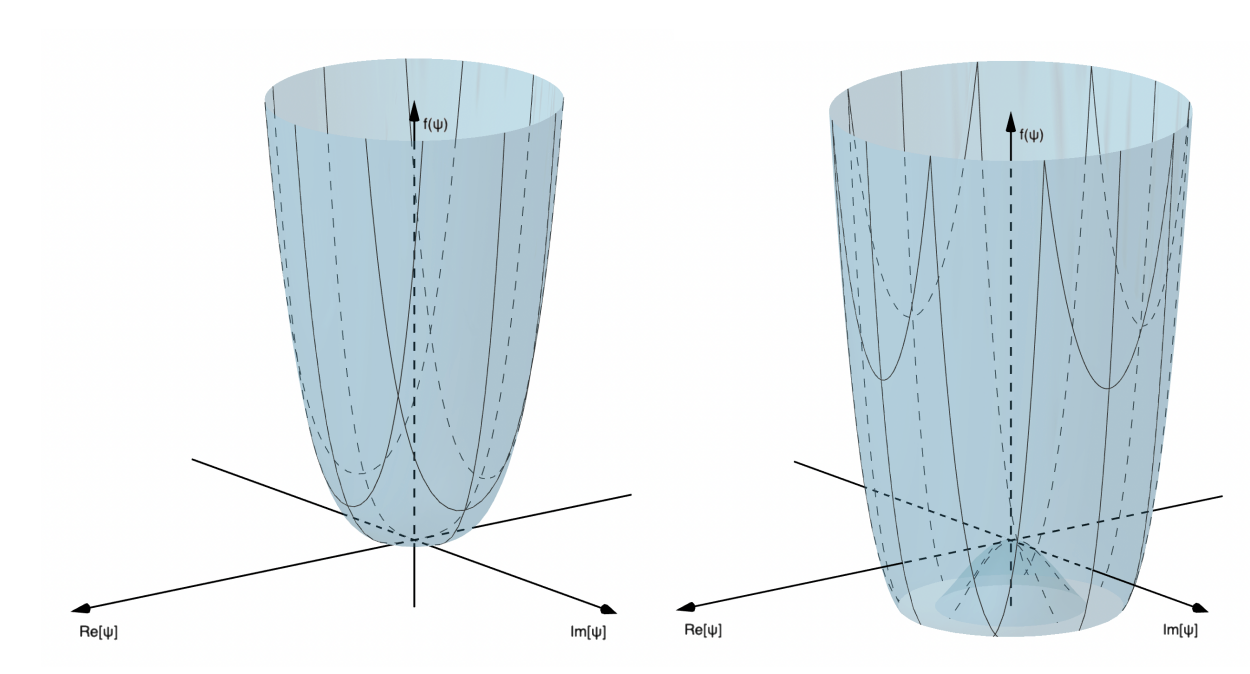
\includegraphics[scale = 0.6]{Chapters/Chapter_5/Images/7_mexican_hat.png}
    \caption{
    Complex order parameter $\Psi$. For $T > T_c$ (left), the potential has a single minimum at $\Psi = 0$, corresponding to the symmetric (normal) phase. For $T < T_c$ (right), the potential develops a continuous circle of degenerate minima at $|\Psi| = \sqrt{-a/b}$.
    }
    \label{fig:mexican_hat_GL}
\end{figure}

\subsection*{Inclusion of spatial variations and magnetic field}
In real materials, the order parameter is not uniform: its amplitude and phase can vary in space, particularly near surfaces, defects, or under the influence of magnetic fields.  
These spatial variations give rise to additional kinetic energy to the free energy, represented by a gradient term proportional to $|\nabla\Psi|^2$.  
Moreover, since the superconducting condensate carries charge, its momentum couples to the electromagnetic field through the \textit{minimal coupling} substitution\footnote{%
In principle, one could also include a scalar electric potential $\phi$ in the coupling, 
but for steady-state situations in a superconductor the perfect conductivity condition 
eliminates any static potential differences.  
Hence, $\phi$ can be neglected here.  
In dynamic situations, such as moving vortices, $\phi$ must be retained, 
but this lies beyond the static Ginzburg--Landau formulation considered in this chapter.%
}:
\[
\mathbf{p} \;\longrightarrow\; \mathbf{p} - q\mathbf{A},
\]
which corresponds to replacing the ordinary derivative by the \emph{gauge-covariant derivative}:
\[
\nabla \;\longrightarrow\; \nabla - i\frac{q}{\hbar}\mathbf{A},
\]
where $q = 2e$ is the charge of a Cooper pair and $\mathbf{A}$ is the magnetic vector potential.\\
Including these effects, the free energy functional becomes
\begin{equation}
F_s = F_n + \int d^3r
\left[
\frac{1}{2m^*}\bigl|(-i\hbar\nabla - q\mathbf{A})\Psi\bigr|^2
+ a(T)|\Psi|^2 + \frac{b(T)}{2}|\Psi|^4
\right],
\label{eq:GL_functional_noBfield}
\end{equation}
where $m^* = 2m_e$ is the effective mass of a Cooper pair.\\
The magnetic field itself also stores energy, given by the usual Maxwell term:
\[
\int d^3r\, \frac{|\mathbf{B}(\mathbf{r})|^2}{2\mu_0}
= \int d^3r\, \frac{(\nabla\times\mathbf{A})^2}{2\mu_0}.
\]
Adding this contribution yields the complete \emph{Ginzburg--Landau free energy functional}:
\begin{equation}
\boxed{
F_s = F_n + \int d^3r
\left\{
\frac{1}{2m^*}\bigl|(-i\hbar\nabla - q\mathbf{A})\Psi\bigr|^2
+ a(T)|\Psi|^2
+ \frac{b(T)}{2}|\Psi|^4
+ \frac{|\nabla\times\mathbf{A}|^2}{2\mu_0}
\right\}}\,.
\label{eq:GL_full_free_energy}
\end{equation}

Equation~\eqref{eq:GL_full_free_energy} describes the macroscopic behaviour of a superconductor through its order parameter and electromagnetic field.  
The first term represents the kinetic energy associated with spatial variations of the condensate, the next two describe the condensation energy, and the last term accounts for the magnetic-field energy.

Minimizing this functional with respect to $\Psi^*$ and $\mathbf{A}$ yields the coupled \emph{Ginzburg--Landau equations}, governing the spatial evolution of the superconducting order parameter and electromagnetic fields.

\section{The Ginzburg--Landau Equations}
\label{sec:GL_equations}

The Ginzburg--Landau free energy functional introduced in Eq.~\eqref{eq:GL_full_free_energy}
can be treated as a variational energy functional whose stationary configuration corresponds
to the equilibrium superconducting state.  
Minimizing it with respect to the complex conjugate of the order parameter $\Psi^*(\mathbf{r})$
and to the vector potential $\mathbf{A}(\mathbf{r})$ yields two coupled differential equations,
known as the \textit{Ginzburg--Landau equations}.

\subsection*{First Ginzburg--Landau equation}

The first equation follows from requiring that the free energy $F_s$ 
be stationary under infinitesimal variations of the complex order parameter.  
In this context, varying the functional with respect to $\Psi^*(\mathbf r)$ 
means determining how the free energy changes when the condensate wavefunction 
$\Psi(\mathbf r)$ and its conjugate $\Psi^*(\mathbf r)$ are independently perturbed.\\
Formally, the stationarity condition is expressed as\footnote{%
In variational problems involving complex fields, such as the superconducting order parameter, 
the field $\Psi$ and its complex conjugate $\Psi^*$ are treated as formally independent variables. 
Since the Ginzburg--Landau free energy $F_s[\Psi,\Psi^*]$ depends on both, one must require 
$\delta F_s/\delta\Psi = 0$ and $\delta F_s/\delta\Psi^* = 0$ for stationarity. 
These two conditions are complex conjugates of each other; 
it is customary to vary with respect to $\Psi^*$, which yields the equation of motion for $\Psi$.}:
\begin{equation}
\frac{\delta F_s}{\delta \Psi^*(\mathbf{r})} = 0,
\label{eq:GL_variation_Psi}
\end{equation}
ensuring that the free energy is stationary under small variations of $\Psi^*$.  
In analogy with classical variational principles, this condition defines the equilibrium configuration of the superconducting condensate.\\
Performing the functional derivative\footnote{%
For the full detailed derivation, see Appendix~\ref{app:GL-derivation}, 
Section~\ref{app:1_GL-derivation}.} 
of Eq.~\eqref{eq:GL_full_free_energy} gives
\begin{equation}
\boxed{
-\frac{\hbar^2}{2m^*}
\left(\nabla - i\frac{q}{\hbar}\mathbf{A}\right)^{\!2}\Psi(\mathbf{r})
+ a(T)\Psi(\mathbf{r})
+ b(T)|\Psi(\mathbf{r})|^2\Psi(\mathbf{r}) = 0.
}
\label{eq:first_GL_eq}
\end{equation}

This nonlinear equation governs the spatial behaviour of the superconducting order parameter 
in the presence of electromagnetic fields.  
The first term represents the kinetic energy associated with spatial variations of $\Psi$, 
the second describes the local condensation energy, and the cubic term 
$b(T)|\Psi|^2\Psi$ accounts for self-interaction between Cooper pairs.  
Together, they describe how both the amplitude and phase of the macroscopic 
wavefunction adjust to minimize the total free energy.

\subsection*{Supercurrent and the Second Ginzburg--Landau Equation}
The second equation follows from requiring the free energy to be stationary under infinitesimal variations of the vector potential~$\mathbf{A}(\mathbf{r})$.
The vector potential is not a fixed external field, it interacts with the superconducting condensate\footnote{%
The magnetic field depends on the current, and the current depends on the magnetic field.}, and the two must be determined self-consistently.
To understand how the magnetic field behaves inside the material, we examine how the free energy changes when $\mathbf A$ is varied.

The free energy depends on the vector potential $\mathbf A$ in two ways:
through the magnetic-field energy term $(|\nabla\times\mathbf A|^2)$, and through its coupling to the superconducting condensate $(|(-i\hbar\nabla - q\mathbf A)\Psi|^2)$.
If $\mathbf A$ changes, both the magnetic field and the kinetic energy of the condensate change, thereby modifying the total free energy of the system.\\
To describe this response quantitatively, we introduce the supercurrent density $\mathbf{J}_s$, defined as the functional derivative of the free energy with respect to $\mathbf A$:
\begin{equation}
\mathbf{J}_s(\mathbf r) = -\,\frac{\delta F_s}{\delta \mathbf A(\mathbf r)}.
\label{eq:Js_variational_def_main}
\end{equation}
Physically, this means that $\mathbf{J}_s$ measures how the system reacts when the magnetic field (or equivalently $\mathbf A$) is varied.
The supercurrent acts as the source of the magnetic field inside the superconductor, and the two quantities influence one another: changing the magnetic field changes the current, and vice versa.\\
A small variation of $\mathbf A$ therefore produces a corresponding change in free energy,
\[
\delta F_s = -\!\int \mathbf J_s \cdot \delta\mathbf A\, d^3r,
\]

\paragraph{Expression for the supercurrent.}
Evaluating the derivative\footnote{%
For the full detailed derivation, see Appendix~\ref{app:GL-derivation}, 
Section~\ref{app:2_GL-derivation}.} in Eq.~\eqref{eq:Js_variational_def_main} for the GL functional gives
\begin{equation}
\boxed{
\mathbf{J}_s =
\frac{i q \hbar}{2 m^*}\bigl(\Psi\,\nabla\Psi^* - \Psi^*\,\nabla\Psi\bigr)
- \frac{q^2}{m^*}|\Psi|^2\mathbf{A}.
}
\label{eq:Js_expression_main}
\end{equation}
The first term arises from gradients in the phase of $\Psi$,
while the second represents the coupling of the condensate to the electromagnetic potential $\mathbf A$.

\paragraph{Phase representation and superfluid velocity.}
Expressing $\Psi = |\Psi| e^{i\theta}$, with $|\Psi|$ constant, makes the structure of the current transparent:
\[
\mathbf{J}_s
= \frac{q\hbar}{m^*}\,|\Psi|^2
\left(\nabla\theta - \frac{q}{\hbar}\mathbf A\right).
\]
The term in parentheses is a gauge-invariant momentum per unit $\hbar$, 
which vanishes when the local phase gradient compensates the electromagnetic potential.  
It is natural to define from it the \emph{superfluid velocity} of the Cooper pairs:
\begin{equation}
\mathbf v_s = \frac{\hbar}{m^*}
\left(\nabla\theta - \frac{q}{\hbar}\mathbf A\right),
\end{equation}
so that $\mathbf J_s = q\,|\Psi|^2\,\mathbf v_s$
takes the same form as the current density of a charged fluid with density $|\Psi|^2$ and charge $q$.
The vector $\mathbf v_s$ therefore describes the collective motion of the condensate,
and spatial variations of the phase $\theta(\mathbf r)$ correspond to macroscopic supercurrents.

\paragraph{Second Ginzburg--Landau equation.}
The magnetic field obeys Ampère’s law,
\[
\nabla\times\mathbf B = \mu_0(\mathbf J_s + \mathbf J_{\rm ext}),
\qquad \mathbf B = \nabla\times\mathbf A,
\]
and substituting Eq.~\eqref{eq:Js_expression_main} gives
\begin{equation}
\boxed{
\nabla \times (\nabla \times \mathbf{A})
= \mu_0
\left[
\frac{i q \hbar}{2 m^*}
\bigl(\Psi\,\nabla\Psi^* - \Psi^*\,\nabla\Psi\bigr)
- \frac{q^2}{m^*}|\Psi|^2\mathbf{A}
+ \mathbf{J}_{\text{ext}}
\right].
}
\label{eq:second_GL_eq_main}
\end{equation}

\bigskip
Together, Eqs.~\eqref{eq:first_GL_eq} and~\eqref{eq:second_GL_eq_main}
form a closed system describing the self-consistent interaction 
between the superconducting condensate and the electromagnetic field.

A vital outcome of these equations is the determination of two intrinsic material length scales: the coherence length ($\xi$) and the magnetic penetration depth ($\lambda$). The ratio of these two lengths, known as the Ginzburg--Landau parameter ($\kappa = \lambda / \xi$), acts as a single, decisive parameter. This dimensionless parameter $\kappa$ determines the fundamental way a superconductor responds to an applied magnetic field and is used to gather different behaviours, leading to the classification of superconducting materials into two distinct groups: \textbf{Type I and Type II superconductors}.


%\subsection{Empirical determination of GL parameters}

\section{Magnetic Penetration Depth and Coherence \\Length}

Before discussing the classification of superconductors, it is useful to introduce
two intrinsic characteristic lengths that naturally arise within the
Ginzburg–Landau theory:
\begin{itemize}
    \item the \textbf{magnetic penetration depth}~$\lambda$, which measures how far
    magnetic fields can penetrate into a superconductor before being screened by
    supercurrents;
    \item the \textbf{coherence length}~$\xi$, which characterizes the typical
    distance over which the order parameter $\Psi$ can vary spatially.
\end{itemize}
These two fundamental scales describe the balance between magnetic and
condensate energies in the superconducting state.  
Their ratio,
\begin{equation}
\kappa = \frac{\lambda}{\xi},
\end{equation}
known as the \textit{Ginzburg--Landau parameter}, plays a decisive role in determining
the magnetic response of a superconductor.  
In the following subsections, we derive explicit expressions for $\lambda$ and $\xi$,
which will later allow us to distinguish between Type~I and Type~II superconductors.


\subsection*{Magnetic Penetration Depth $\lambda$}
\label{sec:penetration_depth}

The first intrinsic length scale obtained from the Ginzburg–Landau theory is the
\textit{magnetic penetration depth}~$\lambda$. This parameter measures how far a magnetic field can penetrate into a superconductor before being exponentially screened by supercurrents, and we will show that it is equivalent to the \textit{London penetration depth} $\lambda_L$ introduced in Section \ref{Lond_eq}.

\paragraph{London limit.}
Let us start from the general expression for the supercurrent density:
\[
\mathbf{J}_s =
\frac{i q \hbar}{2 m^*}
\bigl(\Psi\,\nabla\Psi^* - \Psi^*\,\nabla\Psi\bigr)
- \frac{q^2}{m^*}|\Psi|^2\mathbf{A}.
\]
In the case of a uniform condensate (the so-called London limit, where spatial variations of $|\Psi|$ are negligible), the amplitude $|\Psi|$ is constant. Furthermore, in a situation where the phase is uniform ($\nabla\theta = 0$), the superflow contribution (the first term, related to the gradient of the phase) vanishes. The current density then reduces to the simple form:
\begin{equation}
\mathbf{J}_s = -\,\frac{q^2}{m^*}\,|\Psi|^2\,\mathbf{A}.
\label{eq:london_current_GL}
\end{equation}
This expression corresponds exactly to the microscopic form of the \textit{first London equation}\footnote{%
Originally derived in Section~\ref{Lond_eq}, Eq.~\eqref{000}.},
here obtained directly from the Ginzburg--Landau order parameter~$\Psi$.

\paragraph{Derivation.}
By substituting this GL-derived London current [Eq.~\eqref{eq:london_current_GL}] into Ampère’s law ($\nabla\times\mathbf{B} = \mu_0\,\mathbf{J}_s$), the resulting differential equation for the magnetic field $\mathbf{B}$ is mathematically identical to the London differential equation derived in Section \ref{Lond_eq}:
\begin{equation}
\nabla^2\mathbf{B}
= \frac{1}{\lambda^2}\,\mathbf{B}.
\label{eq:GL_london_equation}
\end{equation}
This confirms that the magnetic field decays exponentially ($\mathbf{B}(x) \propto e^{-x/\lambda}$) over the characteristic length $\lambda$, which is defined by the parameters of the Ginzburg-Landau order parameter:
\begin{equation}
\boxed{
\lambda^2 = \frac{m^*}{\mu_0 q^2 |\Psi|^2}.
}
\label{eq:penetration_depth_GL}
\end{equation}
This result demonstrates the consistency between the Ginzburg–Landau and London descriptions, identifying $\lambda$ with the London penetration depth $\lambda_L$.

\subsection*{Coherence Length}
The coherence length $\xi$ follows from the linearized form of the first Ginzburg–Landau equation in absence of magnetic fields ($\mathbf A=0$), where the order parameter $\Psi$ is small, typically near the critical temperature $T_c$. This length scale characterizes the distance over which $\Psi$ can vary spatially within the superconductor.

\paragraph{Derivation.}

In the zero field case ($\mathbf A=0$), the first GL equation reads
\[
-\frac{\hbar^2}{2m^*}\,\nabla^2 \Psi + a(T)\,\Psi + b(T)\,|\Psi|^2\Psi = 0.
\]
Close to $T_c$ the order parameter is small, so the cubic term can be neglected, giving the linearized equation
\[
-\frac{\hbar^2}{2m^*}\,\nabla^2 \Psi + a(T)\,\Psi \simeq 0
\quad\Longrightarrow\quad
\nabla^2 \Psi = \frac{2m^*\,a(T)}{\hbar^2}\,\Psi.
\]
For $T<T_c$ one has $a(T)<0$, and spatial deviations of $\Psi$ relax exponentially. Defining the characteristic length $\xi$ by
\[
\nabla^2 \Psi = -\frac{1}{\xi^2}\,\Psi,
\]
and using $|a(T)|=-a(T)$ below $T_c$, one obtains
\begin{equation}
\frac{1}{\xi^2}=\frac{2m^*\,|a(T)|}{\hbar^2}
\quad\Longrightarrow\quad
\boxed{\;\xi(T)=\sqrt{\frac{\hbar^2}{2m^*\,|a(T)|}}\, .\;}
\end{equation}

\section{Type I and Type II Superconductors}
\label{sec:type_I_II}

Superconductors can be classified into two fundamental categories, \textit{Type I} and \textit{Type II}, according to their magnetic behaviour in an external field.\\
This distinction arises naturally from the Ginzburg–Landau theory, through the dimensionless parameter
\[
\kappa = \frac{\lambda}{\xi}.
\]
The parameter $\kappa$ represents the relative balance between magnetic and condensation energies:
it compares the characteristic distance over which magnetic fields are screened ($\lambda$) 
with the distance over which the order parameter recovers its bulk value ($\xi$).  

\begin{itemize}
  \item For $\kappa < 1/\sqrt{2}$, the energy cost of forming a normal–superconducting boundary is \emph{positive}, and magnetic flux is completely expelled until the superconducting state abruptly collapses at a single critical field $H_c$.  
  Materials of this kind are called \textbf{Type I superconductors}.
  \item For $\kappa > 1/\sqrt{2}$, the interface energy becomes \emph{negative}, and the system favours the penetration of magnetic flux in the form of quantized vortices.  
  These materials are called \textbf{Type II superconductors}.
\end{itemize}

Thus, $\kappa = 1/\sqrt{2}$ defines the boundary between the two regimes.  
The difference in magnetic behaviour between Type~I and Type~II superconductors follows directly from this energetic balance and is reflected in their magnetization response, shown in Fig.~\ref{fig:typeI_typeII_magnetization}.  

\begin{figure}[H]
\centering
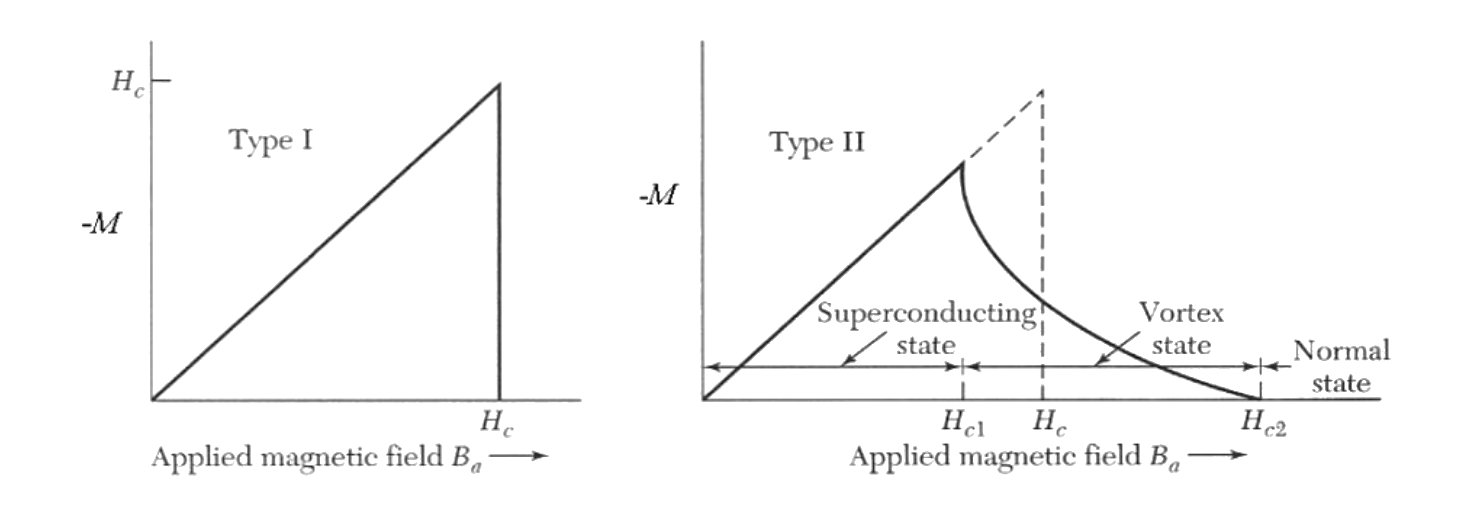
\includegraphics[scale=0.6]{Chapters/Chapter_5/Images/4_type1_type2_2.png}
\caption{
Magnetization curves for Type~I (left) and Type~II (right) superconductors.
Adapted from \cite{raes2021}.
}
\label{fig:typeI_typeII_magnetization}
\end{figure}

In Type~I superconductors, the magnetic field is completely expelled up to the critical field $H_c$, where superconductivity collapses abruptly.  
In Type~II materials, magnetic flux penetrates progressively between two critical fields, $H_{c1}$ and $H_{c2}$, giving rise to an intermediate \textit{mixed state} where normal and superconducting regions coexist, as illustrated in Fig.~\ref{fig:typeI_typeII_magnetizatic_field}.

\begin{figure}[H]
\centering
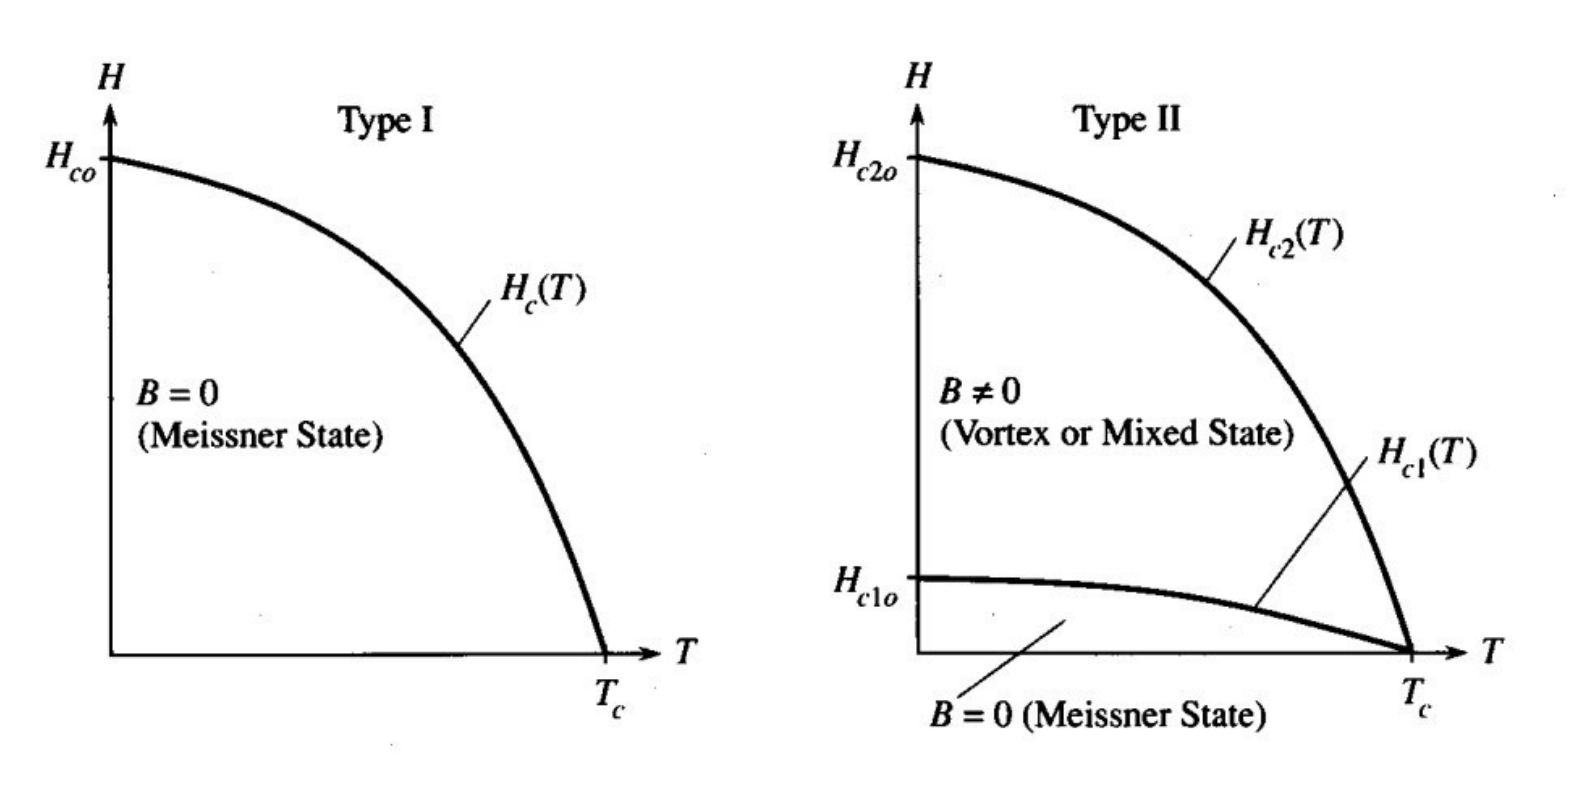
\includegraphics[scale=0.45]{Chapters/Chapter_5/Images/5_states.png}
\caption{
Schematic illustration of magnetic field penetration in Type~I and Type~II superconductors.  
Type~I materials exhibit complete flux expulsion up to $H_c$, while in Type~II materials quantized flux lines penetrate between $H_{c1}$ and $H_{c2}$, forming the mixed (vortex) state.  \\
Image adapted from \cite{raes2021}.
}
\label{fig:typeI_typeII_magnetizatic_field}
\end{figure}

\subsection*{Type I Superconductors}

Type I superconductors are characterized by complete magnetic flux expulsion up to a single critical magnetic field $H_c$.  
For applied fields $H < H_c$, the material remains entirely in the superconducting state, exhibiting perfect diamagnetism ($\mathbf{B}=0$ in the bulk) as a manifestation of the Meissner effect.  
When the field reaches $H_c$, the superconducting state collapses abruptly, and the material transitions uniformly to the normal state.

From an energetic perspective, the interface between a superconducting region and a normal one involves two opposing contributions:
\begin{enumerate}
    \item the \textit{condensation energy gain} $\varepsilon_C$, associated with the formation of the superconducting state, extending over a distance $\xi$;
    \item the \textit{magnetic energy cost} $\varepsilon_B$, associated with expelling the magnetic field, extending over the penetration depth $\lambda$.
\end{enumerate}
In Type I superconductors ($\xi > \lambda$), the magnetic energy cost dominates, leading to a \textit{positive surface energy}. The system thus avoids forming interfaces, preferring to remain either entirely superconducting or entirely normal.  
This explains the single critical field and the absence of partial flux penetration.

\begin{figure}[H]
\centering
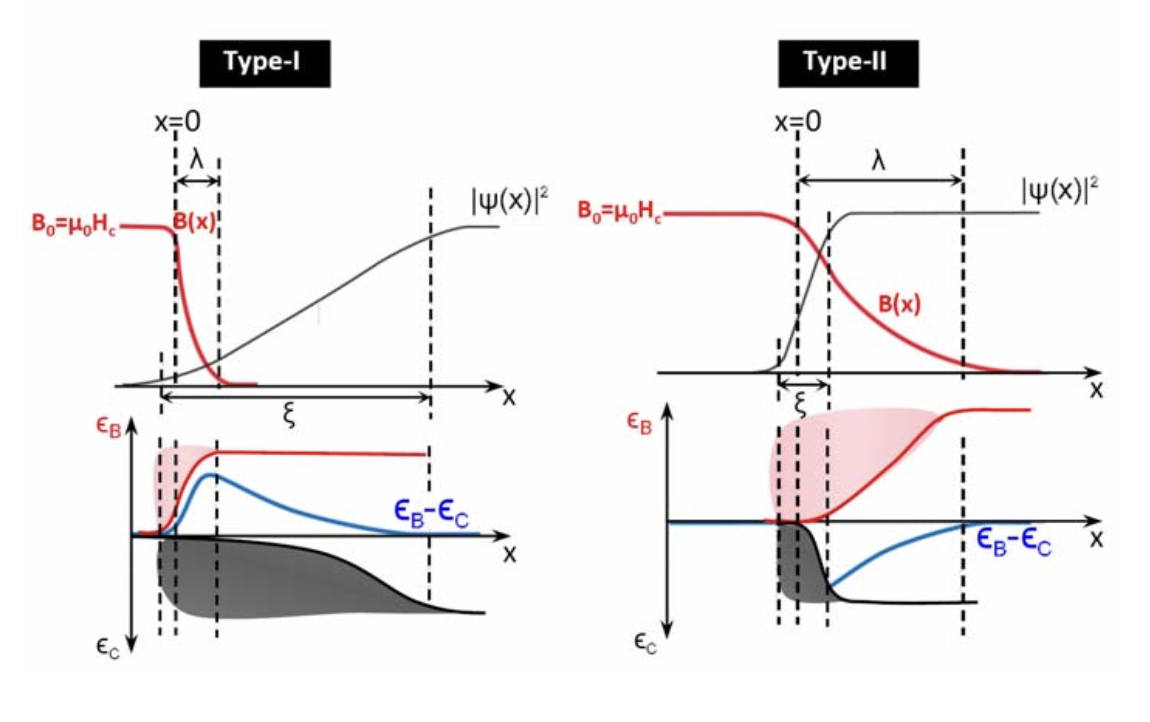
\includegraphics[scale = 0.8]{Chapters/Chapter_5/Images/1_type_1_2.png}
\caption{
Magnetic field (red), order parameter $|\Psi(x)|^2$ (black), and interfacial energy balance for Type I (left) and Type II (right) superconductors.
In Type I materials ($\xi > \lambda$), the interface energy is positive: magnetic flux is completely expelled until the superconducting state collapses at $H_c$.\\
Image adapted from \cite{raes2021}.
}
\label{fig:typeI_typeII_interface}
\end{figure}

The top panels of Fig.~\ref{fig:typeI_typeII_interface} illustrate how, in a Type I material, the magnetic field decays over $\lambda$ while the order parameter recovers over $\xi$.  
The bottom panels show the corresponding energy densities: in the Type I case, the magnetic energy $\varepsilon_B$ exceeds the condensation energy $\varepsilon_C$, making $\varepsilon_B - \varepsilon_C > 0$, i.e.\ interface formation is energetically unfavourable.

Experimentally, Type I superconductors show a sharp transition in their magnetization curve at $H_c$.  
Below $H_c$, the magnetization decreases linearly with the applied field ($\mathbf{B}=0$), whereas above $H_c$ superconductivity is destroyed and $\mathbf{B}=\mu\mathbf{H}$, as shown in Fig.~\ref{fig:typeI_typeII_magnetization}.  
This behaviour is typical of elemental metals such as Pb, Hg, Sn, and Al, which exhibit low critical fields (tens of mT) and critical temperatures below $7$~K.

\subsection*{Type II Superconductors}

Type II superconductors exhibit a richer magnetic behaviour due to their negative interface energy ($\lambda > \xi$).  
At low fields, they behave identically to Type I materials: magnetic flux is completely expelled, and the Meissner effect is preserved.  
However, as the applied field increases, the energetic balance at the boundary between the normal and superconducting regions changes.  
In this case, the magnetic energy gained by allowing partial field penetration over a distance $\lambda$ exceeds the condensation energy cost associated with suppressing the order parameter over $\xi$ (see Fig.~\ref{fig:typeI_typeII_interface}).  
The total surface energy therefore becomes negative, so that the formation of normal–superconducting interfaces lowers the total free energy.  
The system thus finds it energetically favourable to let magnetic flux enter locally, forming many small normal regions embedded in a superconducting matrix.  

\paragraph{Vortices and the Abrikosov lattice.}
When the applied magnetic field exceeds a first critical value $H_{c1}$, magnetic flux begins to penetrate the material in discrete, quantized filaments known as \textit{vortices}.  
These vortices correspond to tiny cylindrical regions where the superconducting order parameter $\Psi$ vanishes and the magnetic field is locally concentrated.  
Between the lower and upper critical fields, $H_{c1}$ and $H_{c2}$, the superconductor enters the so-called \textit{mixed state}, in which normal and superconducting regions coexist.  


\begin{figure}[H]
\centering
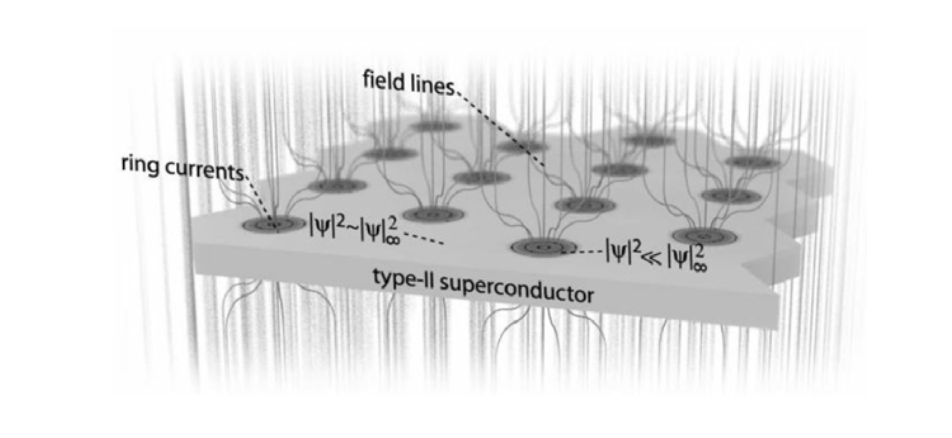
\includegraphics[scale = 0.72]{Chapters/Chapter_5/Images/3_abrikosov.png}
\caption{
An Abrikosov lattice of vortices in a Type~II superconductor.\\
Image adapted from \cite{moshchalkov2011}.
}
\label{fig:abrikosov_lattice}
\end{figure}
As the field increases, the vortices interact repulsively and arrange themselves into a regular, periodic pattern, the \textit{Abrikosov lattice}, which minimizes the total free energy by balancing magnetic and condensation energies.
This ordered structure is characteristic of Type~II superconductivity and is illustrated in Fig.~\ref{fig:abrikosov_lattice}.  \\
As the applied field approaches $H_{c2}$, the density of vortices grows until their cores overlap, at which point superconductivity is completely destroyed and the material becomes normal.\\
Each vortex carries one quantum of magnetic flux,
\begin{equation}
\Phi_0 = \frac{h}{2e},
\end{equation}
and is surrounded by circulating supercurrents that decay over the London penetration depth~$\lambda$.  
The detailed internal structure of a single vortex is shown in Fig.~\ref{fig:vortex_structure}: the magnetic field $B(r)$ peaks at the vortex centre, where $|\Psi|^2$ vanishes, and both quantities recover their bulk values over a characteristic distance $\xi$.

\begin{figure}[H]
\centering
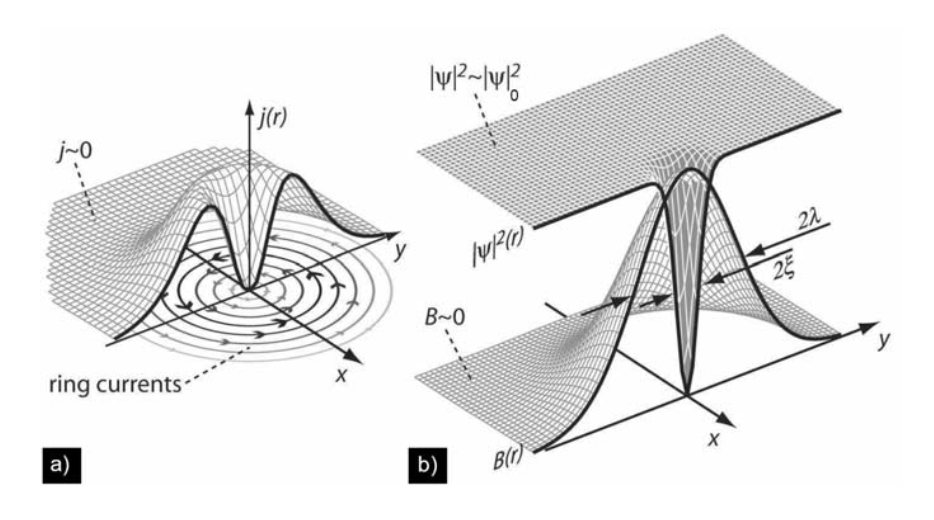
\includegraphics[scale = 0.8]{Chapters/Chapter_5/Images/2_vortex.png}
\caption{
Spatial structure of a single vortex in a Type~II superconductor.  
(a) The supercurrent density forms circular loops around the vortex core and decays on the length scale $\lambda$.  
(b) The order parameter $|\Psi|^2$ vanishes at the vortex centre and recovers over $\xi$, while the magnetic field $B(r)$ peaks in the core and decays outward.  \\
Image adapted from \cite{raes2021}.
}
\label{fig:vortex_structure}
\end{figure}

Type~II superconductors include metallic alloys (NbTi, Nb$_3$Sn) and high-temperature cuprates (YBa$_2$Cu$_3$O$_{7-x}$), which maintain superconductivity under extremely high magnetic fields, up to several tens of tesla, making them essential for technological applications such as particle accelerators.

To highlight the main differences in material properties and critical parameters, 
Table~\ref{tab:typeI_typeII_materials} summarizes representative examples of both Type~I and Type~II superconductors.

\begin{table}[H]
\centering
\renewcommand{\arraystretch}{1.2}
\setlength{\tabcolsep}{5pt}
\small
\begin{tabular}{lccc|lcc}
\hline
\multicolumn{3}{c|}{\textbf{Type I Superconductors}} & 
\multicolumn{3}{c}{\textbf{Type II Superconductors}} \\[2pt]
\textbf{Material} & $T_c$ [K] & $H_c$ [mT] &
\textbf{Material} & $T_c$ [K] & $H_{c2}$ [T] \\ 
\hline
Aluminium (Al)     & 1.2  & 10   & Niobium (Nb)          & 9.3   & 0.4  \\
Tin (Sn)           & 3.7  & 30   & Nb--Titanium (NbTi)   & 9.2   & 14   \\
Lead (Pb)          & 7.2  & 80   & Nb--Tin (Nb$_3$Sn)    & 18    & 25   \\
Mercury (Hg)       & 4.2  & 41   & Vanadium (V)          & 5.3   & 0.9  \\
Zinc (Zn)          & 0.9  & 5    & YBa$_2$Cu$_3$O$_{7-x}$ (YBCO) & 92 & $>100$ \\
\hline
\end{tabular}
\caption{
Representative examples of Type~I and Type~II superconductors with typical critical parameters. 
}
\label{tab:typeI_typeII_materials}
\end{table}


\subsection*{The Emergence of Type III Superconductors}
Beyond the conventional dichotomy of Type~I and Type~II superconductors, recent theoretical developments and experimental observations have revealed superconducting behaviours that do not fit neatly within this traditional classification.
In particular, certain materials display magnetic and transport characteristics that cannot be fully explained by the standard Ginzburg–Landau framework or by the simple $\kappa$-based criterion distinguishing the two known types.

To account for these unconventional phenomena, the concept of a \textbf{Type~III superconductor} has been introduced. These materials exhibit several distinctive physical characteristics that set them apart from conventional superconductors:

\begin{itemize}
    \item \textbf{Inhomogeneous structure:} Type III materials consist of microscopic superconducting regions (or ``droplets'') separated by non-superconducting or weakly superconducting barriers.  
    Their macroscopic superconducting properties emerge from the collective coupling of these regions, rather than from a uniform condensate.
    \item \textbf{Beyond Ginzburg–Landau theory:}  
    The behaviour of these systems cannot be fully captured within the conventional Ginzburg–Landau formalism. Their superconducting properties arise from collective and spatially nonuniform effects that lie beyond the assumptions of a continuous, homogeneous order parameter.
    \item \textbf{Coreless vortices:} In contrast to the \textbf{Abrikosov vortices} of Type II superconductors, which possess a normal (non-superconducting) core of size $\xi$, the vortices in Type III materials are predicted to be \textbf{coreless} (Josephson vortices).  
    These arise in weakly coupled granular or layered systems, where superconducting phase coherence persists without a normal core.
    \item \textbf{Dissipationless transport:} Because these vortices lack a normal core, their motion does not produce resistive dissipation.  
    This feature enables \textbf{lossless current flow} even in the presence of strong magnetic fields, offering potential advantages over conventional Type II superconductors in high-field applications.
\end{itemize}

The emergence of Type III superconductivity thus extends the traditional classification of superconductors, highlighting how material granularity, multi-component order parameters, and topological effects can lead to qualitatively new superconducting phases.  



%%%%%%%%%%%%%%%%%%%%%%%%%%%%%%%%%%%%%%%%%%%%%%%%%%%%%%%%%%%%%%%%%%%%%%%%%%%%%%%%%%%%%%%%%%%%%
%                                    APPENDIX                                          %
%%%%%%%%%%%%%%%%%%%%%%%%%%%%%%%%%%%%%%%%%%%%%%%%%%%%%%%%%%%%%%%%%%%%%%%%%%%%%%%%%%%%%%%%%%%%%
\appendix
\label{Appendix - Calculations}
%================================================================
%================================================================

\chapter{Derivations for Chapter 1}
\label{app:supercond-derivation}
\section*{Derivation of the London Equation Solutions}
\label{app:london_derivation}

The London differential equation for the magnetic induction $\mathbf{B}$ inside a superconductor is a vector Helmholtz equation:
\begin{equation}
    \nabla^2 \mathbf{B} = \frac{\mathbf{B}}{\lambda_L^2} \implies \left(\nabla^2 - \frac{1}{\lambda_L^2}\right) \mathbf{B} = 0,
    \label{eq:appendix_london_helmholtz}
\end{equation}
where $\lambda_L$ is the London penetration depth. This section demonstrates the solution process for the semi-infinite planar geometry.

\paragraph{Semi-Infinite Planar Solution.}
\label{app:planar_solution}

We consider a superconductor occupying the region $x > 0$ with an external field $\mathbf{H}_0 = H_0 \hat{\mathbf{z}}$ applied parallel to the surface ($x=0$). By symmetry, the internal field $\mathbf{B}$ is uniform in $y$ and $z$ and parallel to the applied field:
$$\mathbf{B}(x) = B_z(x) \hat{\mathbf{z}}.$$\\
Substituting this form into Equation \eqref{eq:appendix_london_helmholtz} causes the vector Laplacian $\nabla^2$ to simplify to the scalar second derivative with respect to $x$:
$$\frac{d^2 B_z}{dx^2} = \frac{B_z}{\lambda_L^2}$$\\
This is a second-order linear ordinary differential equation with constant coefficients. Assuming a solution of the form $B_z(x) = e^{kx}$ yields the characteristic equation $k^2 = 1/\lambda_L^2$, leading to two roots, $k = \pm 1/\lambda_L$. The general solution for $x>0$ is:
$$B_z(x) = A e^{+x/\lambda_L} + C e^{-x/\lambda_L}$$

\paragraph{Boundary and Regularity Conditions}
The coefficients $A$ and $C$ are determined by the physical constraints:
\begin{enumerate}
    \item \textbf{Regularity at Infinity ($x \to \infty$):} For the solution to remain finite and physically represent the Meissner effect (flux expulsion), the growing exponential term must be eliminated:
    $$B_z(x) \to 0 \text{ as } x \to \infty \implies A = 0.$$
    The solution reduces to $B_z(x) = C e^{-x/\lambda_L}$.
    \item \textbf{Boundary Condition at Interface ($x = 0$):} The tangential component of the magnetic field strength ($\mathbf{H}$) is continuous across the boundary. Assuming $\mathbf{B} = \mu\mathbf{H}$ inside the superconductor:
    $$B_z(0) = \mu H_{0, \text{tangential}} = \mu H_0.$$
    Substituting this into the reduced solution:
    $$C e^{0} = \mu H_0 \implies C = \mu H_0.$$
\end{enumerate}

Substituting the coefficient $C$ back into the solution yields the field decay result:
$$\mathbf{B}(x) = \mu H_0\,e^{-x/\lambda_L}\,\hat{\mathbf{z}} = \mathbf{B}_0 \,e^{-x/\lambda_L}\,\hat{\mathbf{z}} $$


%================================================================
\chapter{Derivations for Chapter 2}
\label{app:BCS-derivation}
\section*{Fourier derivation of the Cooper integral equation}
\label{app:cooper_FT}

We start from the relative-coordinate Schr\"odinger equation for two identical electrons
(with reduced mass \(\mu=m/2\))
\begin{equation}
\left[-\frac{\hbar^2\nabla_{\mathbf r}^2}{2\mu}+V(\mathbf r)\right]\psi(\mathbf r)
=\tilde E\,\psi(\mathbf r),
\label{eq:cooper_relative_sch_app}
\end{equation}
obtained after separating centre-of-mass and relative motion in the main text.\\
We adopt
\begin{equation}
\psi(\mathbf{k})=\int d^3 r\, \psi(\mathbf r)\,e^{-i\mathbf k\cdot\mathbf r},
\qquad
\psi(\mathbf r)=\int\!\frac{d^3 k}{(2\pi)^3}\, \psi(\mathbf k)\,e^{i\mathbf k\cdot\mathbf r},
\label{eq:FT_defs_app}
\end{equation}
and similarly
\begin{equation}
    V(\mathbf q)=\int d^3r\,V(\mathbf r)\,e^{-i\mathbf q\cdot\mathbf r}.
    \label{eq:FT_defs_app2}
\end{equation}

Applying \eqref{eq:FT_defs_app} and \eqref{eq:FT_defs_app2} to \eqref{eq:cooper_relative_sch_app} gives, term by term,
\begin{align}
\mathcal{F}\!\left\{-\frac{\hbar^2}{2\mu}\nabla_{\mathbf r}^2 \psi(\mathbf r)\right\}
&= \frac{\hbar^2 k^2}{2\mu}\,\psi(\mathbf k), \nonumber \\[4pt]
\mathcal{F}\!\left\{V(\mathbf r)\psi(\mathbf r)\right\}
%&= \int\!\frac{d^3 k'}{(2\pi)^3}\, V(\mathbf k-\mathbf k')\,\psi(\mathbf k'),\\[4pt]
%\mathcal{F}\!\left\{\tilde E\,\psi(\mathbf r)\right\}
&=  E\,\psi(\mathbf k). \nonumber
\end{align}


For the second term, we recall that the Fourier transform of a product of two functions is given by the convolution of their Fourier transforms:
\[
\mathcal{F}\{f(\mathbf r)g(\mathbf r)\}(\mathbf k)
= \int\!\frac{d^3k'}{(2\pi)^3}\, f(\mathbf k-\mathbf k')\, g(\mathbf k').
\]
Applying this to \(V(\mathbf r)\psi(\mathbf r)\) gives
\[
\mathcal{F}\!\left\{V(\mathbf r)\psi(\mathbf r)\right\}
= \int\!\frac{d^3k'}{(2\pi)^3}\, V(\mathbf k-\mathbf k')\, \psi(\mathbf k').
\]

Collecting all terms gives:
\begin{equation}
\left(\frac{\hbar^2 k^2}{2\mu}\right)\psi(\mathbf k)
+\int\!\frac{d^3 k'}{(2\pi)^3}\, V(\mathbf k-\mathbf k')\,\psi(\mathbf k')
=\tilde E\,\psi(\mathbf k).
\label{eq:momentum_schro_app}
\end{equation}
For two identical electrons: \[\mu=\frac{\mu}{2} ,\quad \implies \quad \frac{\hbar^2 k^2}{2\mu}=\frac{\hbar^2 k^2}{m}\equiv 2\epsilon_{\mathbf k}\, ,\quad  
\epsilon_{\mathbf k}=\frac{\hbar^2 k^2}{2m}.\]
\noindent Rearranging \eqref{eq:momentum_schro_app} yields the \emph{Cooper integral equation}:
\begin{equation}
\boxed{
\bigl( E-2\epsilon_{\mathbf k}\bigr)\,\psi(\mathbf k)
=\int\!\frac{d^3 k'}{(2\pi)^3}\, V(\mathbf k-\mathbf k')\,\psi(\mathbf k')}\, .
\label{eq:cooper_integral_app}
\end{equation}

Define the modified wavefunction
\[
\Delta(\mathbf k)\equiv \bigl(E-2\epsilon_{\mathbf k}\bigr)\,\psi(\mathbf k),
\qquad (E\equiv \tilde E\ \text{for }\mathbf K=0),
\]
to express \eqref{eq:cooper_integral_app} as:
\begin{equation}
\boxed{
\Delta(\mathbf k) = -\!\int\!\frac{d^3 k'}{(2\pi)^3}\;
\frac{V(\mathbf k-\mathbf k')}{\,2\epsilon_{\mathbf k'}-E\,}\;\Delta(\mathbf k')}\, .
\label{eq:cooper_Delta_app}
\end{equation}
Equations \eqref{eq:cooper_integral_app}–\eqref{eq:cooper_Delta_app} represent the Schrödinger equation for the relative motion written in momentum space.
%================================================================

%================================================================
%================================================================
%================================================================
\chapter{Derivations for Chapter 3}
\label{app:BEC-derivation}
\section*{Density of States in Three Dimensions}
\label{density_of_states}

We aim to calculate the density of states \( D(\varepsilon) \), defined as the number of available single–particle states per unit energy, as a function of the energy \( \varepsilon \).

The first step consists in counting the number of allowed states in \(k\)–space for free particles confined in a box of side \(L\) and volume \(V = L^3\), assuming periodic boundary conditions.  
Each quantum state corresponds to a point in \(k\)–space separated from the next by an interval
\[
\Delta k_x = \Delta k_y = \Delta k_z = \frac{2\pi}{L},
\]
so that the elementary volume occupied by one state in \(k\)–space is
\[
\Delta V_k = \left(\frac{2\pi}{L}\right)^3 = \frac{(2\pi)^3}{V}.
\]
Thus, the number of available states in a region of volume \( dV_k \) of \(k\)–space is given by
\[
dN = \frac{1}{\frac{(2\pi)^3}{V}}\,dV_k =  \frac{V}{(2\pi)^3}\,dV_k .
\]
 
The number of \(k\)–states within a spherical shell of radius \(k\) and thickness \(dk\) is proportional to the surface area of the sphere times \(dk\):
\[
dV_k = 4\pi k^2\,dk.
\]
Substituting into the previous expression gives
\[
dN = \frac{V}{(2\pi)^3}\,4\pi k^2\,dk = \frac{V k^2}{2\pi^2}\,dk.
\]

Differentiating the dispersion relation \( \varepsilon = \frac{\hbar^2 k^2}{2m} \), we obtain
\[
d\varepsilon = \frac{\hbar^2 k}{m}\,dk,
\qquad \text{or equivalently} \qquad
dk = \frac{m}{\hbar^2 k}\,d\varepsilon.
\]
Replacing \( dk \) in the expression for \( dN \) yields
\[
dN = \frac{V k^2}{2\pi^2} \cdot \frac{m}{\hbar^2 k}\,d\varepsilon
= \frac{V m k}{2\pi^2 \hbar^2}\,d\varepsilon.
\]

We can express the wavevector magnitude in terms of the particle energy using
\[
k = \sqrt{\frac{2m\varepsilon}{\hbar^2}}.
\]
Substituting this into the previous relation, the density of states per unit energy is obtained as
\begin{equation}
D_{3D}(\varepsilon) = \frac{dN}{d\varepsilon}
= \frac{V}{4\pi^2} \left(\frac{2m}{\hbar^2}\right)^{3/2} \varepsilon^{1/2}.
\end{equation}

\begin{figure}[H]
    \centering
    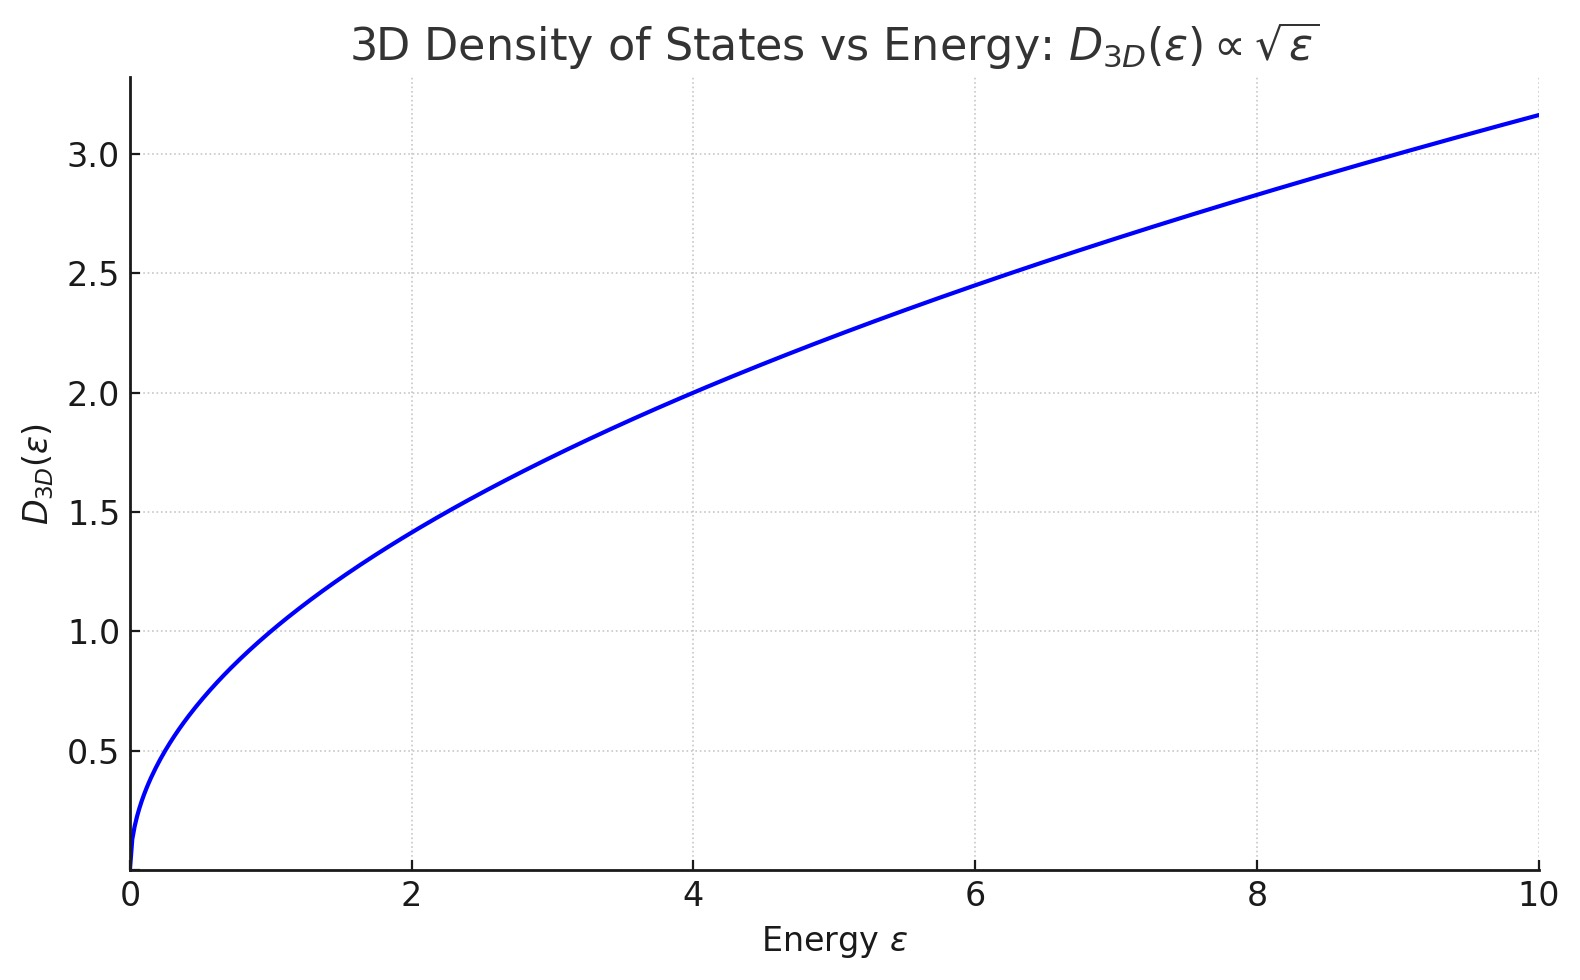
\includegraphics[scale= 0.2]{Chapters/Chapter_2/Images/3_3D.jpg}
    \caption{3D density of states $D_{3D}(\varepsilon)$ as a function of the energy.}
    \label{Figure 5 - DOS}
\end{figure}
%================================================================
\section*{Gamma function and Riemann zeta function}
\label{appendix:gamma_riemann}

In the derivation of the critical density and temperature for Bose--Einstein condensation, two special mathematical functions appear naturally: the \textit{Gamma function} and the \textit{Riemann zeta function}.  
Their properties allow one to evaluate integrals of the type
\[
    \int_0^{\infty} \frac{x^{\alpha - 1}}{e^x - 1}\, dx.
\]

\paragraph{The Gamma Function}

The Gamma function \( \Gamma(\alpha) \) generalizes the factorial function to real and complex arguments.  
It is defined for \( \Re(\alpha) > 0 \) by
\begin{equation}
    \Gamma(\alpha) = \int_0^{\infty} t^{\alpha - 1} e^{-t}\, dt.
    \label{eq:gamma_def}
\end{equation}
It satisfies the recurrence relation
\[
    \Gamma(\alpha + 1) = \alpha\, \Gamma(\alpha),
\]
and for integer values \( n \), it reduces to the factorial:
\[
    \Gamma(n) = (n - 1)!.
\]
Some useful values are
\[
    \Gamma\!\left(\tfrac{1}{2}\right) = \sqrt{\pi},
    \qquad
    \Gamma\!\left(\tfrac{3}{2}\right) = \tfrac{1}{2}\sqrt{\pi}.
\]
The Gamma function often appears in statistical physics when transforming integrals over momentum or energy to integrals over dimensionless variables.

\paragraph{The Riemann Zeta Function}

The Riemann zeta function \( \zeta(\alpha) \) is defined for \( \Re(\alpha) > 1 \) as the infinite series
\begin{equation}
    \zeta(\alpha) = \sum_{n=1}^{\infty} \frac{1}{n^{\alpha}}.
    \label{eq:zeta_def}
\end{equation}
It can also be expressed as:
\begin{equation}
    \zeta(\alpha) = \frac{1}{\Gamma(\alpha)} \int_0^{\infty} \frac{x^{\alpha - 1}}{e^x - 1}\, dx.
\end{equation}
This representation connects \( \zeta(\alpha) \) to integrals encountered in quantum statistics, particularly in the evaluation of thermodynamic quantities for Bose and Fermi gases.

For the case relevant to Bose--Einstein condensation, \( \alpha = 3/2 \), the value is
\[
    \zeta\!\left(\tfrac{3}{2}\right) \approx 2.612.
\]
Combining this with \( \Gamma(3/2) = \tfrac{\sqrt{\pi}}{2} \), the integral
\[
    \int_0^{\infty} \frac{x^{1/2}}{e^x - 1}\, dx
\]
can be evaluated as
\[
    \Gamma\!\left(\tfrac{3}{2}\right) \zeta\!\left(\tfrac{3}{2}\right)
    = \frac{\sqrt{\pi}}{2}\, \zeta\!\left(\tfrac{3}{2}\right)
    \approx 2.315.
\]
This numerical factor directly determines the prefactor in the expression for the critical density and critical temperature of the Bose gas [Eq.~\eqref{eq:nc_result}].

%================================================================
%================================================================
%================================================================
\chapter{Derivations for Chapter 4}
\label{app:BCS_BEC-derivation}
\section*{Critical Temperature for Linear Dispersion}
\label{app:Tc_linear_dispersion}

Starting from the general expression for the critical temperature of a Bose gas with dispersion relation
\[
\varepsilon_K = C_s K^s,
\]
the condensation temperature in \(d\) spatial dimensions is given by Eq.~\eqref{eq:Tc_general_1}:
\begin{equation}
T_c = \frac{C_s}{k_B}
\left[
    \frac{s\, \Gamma(d/2)\, (2\pi)^d\, n_B}
         {2\, \pi^{d/2}\, \Gamma(d/s)\, g_{d/s}(1)}
\right]^{s/d}.
\label{eq:app_Tc_general}
\end{equation}

To obtain the expression corresponding to a \textit{linear dispersion}, we set
\[
s = 1, \qquad \varepsilon_K = \alpha(d)\,\hbar v_F\, K,
\]
where \(\alpha(d)\) is a dimension-dependent numerical factor (\(\alpha(2) = 2/\pi\), \(\alpha(3) = 1/2\)) and \(v_F\) the Fermi velocity.  
Substituting these values into Eq.~\eqref{eq:app_Tc_general}, we find:
\begin{align}
T_c 
&= \frac{\alpha(d)\, \hbar v_F}{k_B}
\left[
    \frac{1 \cdot \Gamma(d/2)\, (2\pi)^d\, n_B}
         {2\, \pi^{d/2}\, \Gamma(d)\, g_d(1)}
\right]^{1/d} \nonumber \\[6pt]
&= \frac{\alpha(d)\, \hbar v_F}{k_B}
\left[
    \frac{\pi^{(d+1)/2}\, n_B}
         {\Gamma\!\left[(d+1)/2\right]\, g_d(1)}
\right]^{1/d}.
\label{eq:app_Tc_linear_final}
\end{align}

Equation~\eqref{eq:app_Tc_linear_final} reproduces Eq.~\eqref{eq:Tc_linear_dispersion} in the main text.  
This result shows that for linear dispersion (\(s=1\)), the critical temperature remains finite for all \(d > 1\), thereby explaining the possibility of condensation, and hence superconductivity, in quasi-two-dimensional systems.
%================================================================
%================================================================

\section*{Recovery of the Conventional 3D Bose–Einstein Critical Temperature}
\label{d3s2}
For a quadratic dispersion \(\varepsilon_K=C_2 K^2\) with \(C_2=\hbar^2/(2M)\) and in \(d=3\) dimensions, Eq.~\eqref{eq:Tc_general_2} gives
\[
T_c \;=\; \frac{C_2}{k_B}
\left[
\frac{s\,\Gamma\!\left(\frac d2\right) (2\pi)^d n_B}
{2\,\pi^{d/2}\,\Gamma\!\left(\frac{d}{s}\right)\,\zeta\!\left(\frac{d}{s}\right)}
\right]^{s/d}
\;=\;
\frac{\hbar^2}{2 M k_B}
\left[
\frac{2\,\Gamma\!\left(\tfrac{3}{2}\right) (2\pi)^3 n_B}
{2\,\pi^{3/2}\,\Gamma\!\left(\tfrac{3}{2}\right)\,\zeta\!\left(\tfrac{3}{2}\right)}
\right]^{2/3}.
\]
Cancelling the \(\Gamma\!\left(\tfrac{3}{2}\right)\) factor yields
\[
\text{bracket}
=
\frac{2\,\Gamma\!\left(\tfrac{3}{2}\right)\, 8\pi^3\, n_B}
     {2\,\pi^{3/2}\,\Gamma\!\left(\tfrac{3}{2}\right)\,\zeta(3/2)}
=
\frac{8\pi^3\, n_B}{\pi^{3/2}\,\zeta(3/2)}
=
\frac{8\,\pi^{3/2}\, n_B}{\zeta(3/2)}.
\]
Raising to the power \(2/3\) gives
\[
\left(\frac{8\,\pi^{3/2}\, n_B}{\zeta(3/2)}\right)^{2/3}
= 8^{2/3}\,\pi^{(3/2)\cdot(2/3)} \left(\frac{n_B}{\zeta(3/2)}\right)^{2/3}
= 4\,\pi \left(\frac{n_B}{\zeta(3/2)}\right)^{2/3}.
\]
Therefore,
\[
T_c
= \frac{\hbar^2}{2 M k_B}\, 4\pi \left(\frac{n_B}{\zeta(3/2)}\right)^{2/3}
= \frac{2\pi \hbar^2}{M k_B}\,
\left[\frac{n_B}{\zeta(3/2)}\right]^{2/3},
\]
which is Eq.~\eqref{eq:Crit_T} (identifying \(n_B \equiv n\) and $M = 2m$).

%================================================================
%================================================================
%================================================================
%========================================================
% Appendix: Variational derivation of the GL equations
%========================================================
\chapter{Derivations for Chapter 5}
\label{app:GL-derivation}

\section*{Setup and notation}
We start from the Ginzburg--Landau free-energy functional:
\begin{equation}
\boxed{
\begin{aligned}
F_s[\Psi,\Psi^*,\mathbf A] = F_n &+ \int_V d^3 r \left[
\frac{1}{2m^*}\, \big|(-i\hbar\nabla - q \mathbf A)\Psi\big|^2 \right] \\
&+ \int_V d^3 r \left[ a(T)\,|\Psi|^2 + \frac{b(T)}{2}\,|\Psi|^4
+ \frac{|\nabla \times \mathbf A|^2}{2\mu_0} \right]
\end{aligned}
\label{app:Fs}
}
\end{equation}
where $q=2e$ and $m^*$ are the charge and effective mass of a Cooper pair.
We treat $\Psi$ and $\Psi^*$ as independent variational fields.\footnote{%
In the variational calculus for complex fields, $\Psi$ and $\Psi^*$ are regarded
as independent variables. One thus obtains one Euler--Lagrange equation from
$\delta F_s / \delta \Psi^* = 0$ and another from $\delta F_s / \delta \Psi = 0$,
which are complex conjugates of each other.}
For compactness, define the \emph{gauge-covariant differential operator}
\[
\hat\Pi \equiv -\,i\hbar\nabla - q\,\mathbf A(\mathbf r),
\qquad
\hat\Pi^\dagger \equiv i\hbar\nabla - q\,\mathbf A(\mathbf r),
\]
so that
\[
\big|(-i\hbar\nabla - q\mathbf A)\Psi\big|^2
= \big(\hat\Pi\Psi\big)^* \cdot \big(\hat\Pi\Psi\big)
= \sum_{j=1}^3 \big[\hat\Pi_j\Psi\big]^* \big[\hat\Pi_j\Psi\big].
\]
We will vary $F_s$ with respect to $\Psi^*$ (first GL equation)
and with respect to $\mathbf A$ (second GL equation). 
Throughout, we assume either $\delta\Psi|_{\partial V}=0$ and $\delta\mathbf A|_{\partial V}=0$,
or boundary conditions that make surface integrals vanish (e.g.\ no normal supercurrent through the boundary).

%------------------------------------------------------------
\section*{Variation with respect to $\Psi^*$: the first GL equation}
%------------------------------------------------------------
\label{app:1_GL-derivation}

By definition, for any infinitesimal variation $\delta\Psi^*$ with compact support,
\[
\delta F_s \;\equiv\; F_s[\Psi,\Psi^*+\delta\Psi^*,\mathbf A]-F_s[\Psi,\Psi^*,\mathbf A]
= \int_V d^3r\; \frac{\delta F_s}{\delta \Psi^*(\mathbf r)}\,\delta\Psi^*(\mathbf r)
\;+\; \text{(surface terms)}.
\]
In this expression, ``surface terms'' refers to possible boundary contributions 
that arise whenever the functional $F_s$ depends on spatial derivatives of the field, 
such as $\nabla\Psi$.\footnote{%
During the variation, these derivative terms lead to integrals of the form 
$\int_V (\nabla \delta\Psi^*) \cdot (\dots)\, d^3r$, which—upon integrating by parts—
generate additional boundary integrals over $\partial V$. 
Under standard boundary conditions (for example, $\delta\Psi^* = 0$ or vanishing normal current at the surface), 
these surface terms vanish, leaving only the volume integral that defines the functional derivative.%
}
Stationarity of $F_s$ under arbitrary $\delta\Psi^*$ (and with boundary terms vanishing)
implies the Euler--Lagrange condition
\begin{equation}
\frac{\delta F_s}{\delta \Psi^*(\mathbf r)} = 0,
\label{eq:EL_condition_Psi}
\end{equation}
which is the \emph{first Ginzburg--Landau equation}.
Below we evaluate $\delta F_s$ explicitly by varying only the $\Psi^*$-dependent terms
and integrating by parts to move derivatives off $\delta\Psi^*$.

\paragraph{(i) Identify the $\Psi^*$--dependent terms.}
From Eq.~\eqref{app:Fs}, only three contributions depend on $\Psi^*$:
\[
\frac{1}{2m^*} \sum_j [\hat\Pi_j\Psi]^* [\hat\Pi_j\Psi],\qquad
a\,|\Psi|^2 = a\,\Psi\Psi^*,\qquad
\frac{b}{2}|\Psi|^4 = \frac{b}{2}(\Psi\Psi^*)^2.
\]

\paragraph{(ii) Variation of the kinetic term.}
Because $\mathbf A$ is held fixed, $\delta(\hat\Pi_j\Psi)=0$, while
\[
[\hat\Pi_j \Psi]^* = (i\hbar \partial_j - q A_j)\Psi^* .
\]
Thus
\[
\delta \left( [\hat\Pi_j\Psi]^* [\hat\Pi_j\Psi] \right)
= \big[(i\hbar \partial_j - q A_j)\,\delta\Psi^*\big]\,[\hat\Pi_j\Psi].
\]
Summing over $j$ and integrating over the volume,
\begin{align}
\delta F_{\rm kin}
&= \int_V d^3r \; \frac{1}{2m^*} \sum_j
\big[(i\hbar \partial_j - q A_j)\,\delta\Psi^*\big]\,[\hat\Pi_j\Psi]  \nonumber \\
&= \int_V d^3r \; \frac{1}{2m^*} \sum_j \big( i\hbar\,\partial_j \delta\Psi^* - q A_j  \delta\Psi^* \big)\,[\hat\Pi_j\Psi]. \nonumber
\end{align}
The first equality follows directly from the \textit{integration by parts theorem} in three dimensions,
which generalizes the one-dimensional identity
\[
\int f'(x)\, g(x)\,dx
= \big[f(x)g(x)\big]_{\text{boundary}} - \int f(x)\, g'(x)\,dx
\]
to vector fields. In differential form, for scalar functions $f(\mathbf r)$ and $g(\mathbf r)$, one has
\[
\int_V (\partial_j f)\, g\, d^3r
= \int_{ V} \partial_j(f g)\,\, dS
- \int_V f\, (\partial_j g)\, d^3r,
%\label{eq:integration_by_parts_3D}
\]
Now, applying Gauss's divergence theorem
\[
\int_V \nabla\!\cdot(f\,\mathbf{g})\,d^3r
= \int_{\partial V} f\,\mathbf{g}\cdot \hat{\mathbf n}\,dS.
\]
to the mid term, we get: 
\begin{equation}
\int_V (\partial_j f)\, g\, d^3r
= \int_{\partial V} f g\, \hat n_j\, dS
- \int_V f\, (\partial_j g)\, d^3r,
\label{eq:integration_by_parts_3D}
\end{equation}


In our case we identify $f = i\hbar\,\delta\Psi^*$ and $g = [\hat\Pi_j\Psi]$.
Applying Eq.~\eqref{eq:integration_by_parts_3D} gives
\[
\int_V (i\hbar\,\partial_j \delta\Psi^*)\, [\hat\Pi_j\Psi]\, d^3r
= \int_{\partial V} dS\, i\hbar\, \delta\Psi^* [\hat\Pi_j\Psi]\hat n_j
- \int_V d^3r\, i\hbar\, \delta\Psi^* \partial_j[\hat\Pi_j\Psi],
\]
where the first term is the \emph{surface contribution} resulting from Gauss’s theorem,
and the second is the \emph{volume term} that remains after transferring the derivative
from $\delta\Psi^*$ onto $[\hat\Pi_j\Psi]$.
Under standard boundary conditions (e.g.\ $\delta\Psi^* = 0$ or vanishing normal supercurrent at $\partial V$),
the surface integral vanishes, leaving only the bulk contribution to the variation.
Assuming the surface term vanishes, we get
\[
\delta F_{\rm kin}
= \int_V d^3r\; \frac{1}{2m^*}\,\delta\Psi^*
\sum_j \Big\{- i\hbar \,\partial_j[\hat\Pi_j\Psi] - q A_j [\hat\Pi_j\Psi]\Big\}.
\]
Recognizing the divergence of the covariant operator,
\[
\sum_j \Big\{- i\hbar \,\partial_j - q A_j\Big\} [\hat\Pi_j\Psi]
= (i\hbar\nabla - q\mathbf A)\cdot(\hat\Pi\Psi)
= \hat\Pi^\dagger \!\cdot\, \hat\Pi \Psi,
\]
we find
\[
\delta F_{\rm kin} = \int_V d^3r\; \delta\Psi^*\;
\frac{1}{2m^*}\, \hat\Pi^\dagger \!\cdot\, \hat\Pi \Psi
= \int_V d^3r\; \delta\Psi^*\;
\frac{1}{2m^*}\, \hat\Pi^2 \Psi,
\]
since $\hat\Pi^\dagger \!\cdot\, \hat\Pi = \hat\Pi^2 \equiv \sum_j \hat\Pi_j \hat\Pi_j$.

\paragraph{(iii) Variation of the potential terms.}
For $a|\Psi|^2 = a\Psi\Psi^*$,
\[
\delta (a\Psi\Psi^*) = a\,\Psi\,\delta\Psi^*,
\quad \Rightarrow \quad
\delta F_a = \int_V d^3r\, a\,\Psi\,\delta\Psi^*.
\]
For $\frac{b}{2}|\Psi|^4 = \frac{b}{2}(\Psi\Psi^*)^2$,
\[
\delta\!\left(\frac{b}{2}(\Psi\Psi^*)^2\right)
= b|\Psi|^2\,\Psi\,\delta\Psi^*,
\quad \Rightarrow \quad
\delta F_b = \int_V d^3r\, b|\Psi|^2\Psi\,\delta\Psi^*.
\]

\bigskip
\noindent\textbf{(iv) Combine all contributions.}
Summing the three variations,
\[
\delta F_s
= \int_V d^3r\, \delta\Psi^*
\left[
\frac{1}{2m^*}\hat\Pi^2\Psi + a\Psi + b|\Psi|^2\Psi
\right].
\]
Since $\delta\Psi^*$ is arbitrary, the integrand must vanish:
\begin{equation}
\boxed{
\frac{1}{2m^*}\,(-i\hbar\nabla - q\mathbf A)^2 \Psi
+ a\,\Psi + b\,|\Psi|^2\Psi = 0,
}
\label{eq:GL1_final}
\end{equation}
which is the \emph{first Ginzburg--Landau equation}.

%========================================================
\section*{Variation with respect to $\mathbf A$: Second GL Equation}
\label{app:2_GL-derivation}
%========================================================

We now derive the second Ginzburg--Landau equation by following the same procedure used for the first one.  
In this case, the functional derivative is taken with respect to the vector potential $\mathbf{A}(\mathbf{r})$, which couples the superconducting condensate to the electromagnetic field.  
Our goal is to compute
\[
\frac{\delta F_s}{\delta \mathbf{A}(\mathbf{r})},
\]
and identify from it the expression for the superconducting current density $\mathbf{J}_s$.  
Only the terms in the free-energy functional that depend explicitly on $\mathbf{A}$ contribute to this variation:
\[
    \frac{|\nabla\times \mathbf A|^2}{2\mu_0}, 
    \qquad 
    \left[
    \frac{1}{2m^*}\, \big|(-i\hbar\nabla - q \mathbf A)\Psi\big|^2
    \right].
\]


\paragraph{(i) Variation of the magnetic energy}
The magnetic term is
\[
F_B[\mathbf A]=\int_V \frac{|\nabla\times \mathbf A|^2}{2\mu_0}\,d^3r
=\frac{1}{2\mu_0}\int_V (\nabla\times\mathbf A)\cdot(\nabla\times\mathbf A)\,d^3r .
\]
Varying,
\[
\delta F_B
=\frac{1}{\mu_0}\int_V (\nabla\times\mathbf A)\cdot(\nabla\times\delta\mathbf A)\,d^3r .
\]
Use the vector identity
\[
(\nabla\times\mathbf A)\cdot(\nabla\times\delta\mathbf A)
= \nabla\!\cdot\!\big[\delta\mathbf A\times(\nabla\times\mathbf A)\big]
+ \delta\mathbf A\cdot\big[\nabla\times(\nabla\times\mathbf A)\big],
\]
and apply the divergence theorem to obtain
\begin{equation}
\delta F_B
= \frac{1}{\mu_0}\int_V \delta\mathbf A\cdot\big[\nabla\times(\nabla\times\mathbf A)\big]\,d^3r
\;+\; \underbrace{\frac{1}{\mu_0}\oint_{\partial V}
\hat{\mathbf n}\cdot\!\big[\delta\mathbf A\times(\nabla\times\mathbf A)\big]\;dS}_{\text{surface term}} .
\label{app:FB-var}
\end{equation}
Under the usual electromagnetic boundary conditions (e.g. fixed tangential \(\mathbf A\) or vanishing \(\delta\mathbf A\) on \(\partial V\)) the surface term vanishes.

\paragraph{(ii) Variation of the kinetic energy}
The kinetic term can be written componentwise as
\[
F_{\rm kin}=\int_V \frac{1}{2m^*}\sum_{j=1}^3 [\hat\Pi_j\Psi]^*[\hat\Pi_j\Psi]\,d^3r .
\]
When only \(\mathbf A\) varies, \(\Psi\) is fixed and
\[
\delta\big(\hat\Pi_j\Psi\big)= -\,q\,\delta A_j\,\Psi,
\qquad
\delta\big([\hat\Pi_j\Psi]^*\big)= -\,q\,\delta A_j\,\Psi^* .
\]
Hence
\begin{align}
\delta F_{\rm kin}
&= \int_V \frac{1}{2m^*}\sum_j
\Big\{ \delta\big([\hat\Pi_j\Psi]^*\big)\,[\hat\Pi_j\Psi]
+ [\hat\Pi_j\Psi]^*\,\delta\big(\hat\Pi_j\Psi\big) \Big\}\,d^3r \nonumber\\
&= -\int_V \frac{q}{2m^*}\sum_j \delta A_j
\Big[ \Psi^*\,(\hat\Pi_j\Psi) + \Psi\,(\hat\Pi_j\Psi)^* \Big]\,d^3r \nonumber .
%\label{app:Fkin-var-raw}
\end{align}
Insert \(\hat\Pi_j\Psi=-i\hbar\,\partial_j\Psi - qA_j\Psi\) and its complex conjugate:
\[
\Psi^*(\hat\Pi_j\Psi) + \Psi(\hat\Pi_j\Psi)^*
= -\,i\hbar\big(\Psi^*\partial_j\Psi - \Psi\,\partial_j\Psi^*\big)
- 2q\,|\Psi|^2 A_j .
\]
Therefore
\begin{align}
\delta F_{\rm kin}
&= \int_V \delta\mathbf A\cdot
\left[
\frac{q\hbar}{2m^* i}\,(\Psi^*\nabla\Psi - \Psi\nabla\Psi^*)
+ \frac{q^2}{m^*}\,|\Psi|^2 \mathbf A
\right] d^3r .
\label{app:Fkin-var-final}
\end{align}
Note that no integration by parts is required here: the dependence on \(\mathbf A\) is algebraic.

\paragraph{(iii) Collecting terms and identifying the supercurrent}
Combining Eqs.~\eqref{app:FB-var} and \eqref{app:Fkin-var-final}, and dropping the surface term,
\begin{equation}
\delta F_s
= \int_V \delta\mathbf A\cdot
\left\{
\frac{1}{\mu_0}\,\nabla\times(\nabla\times\mathbf A)
- \frac{q\hbar}{2m^* i}\,(\Psi^*\nabla\Psi - \Psi\nabla\Psi^*)
+ \frac{q^2}{m^*}\,|\Psi|^2 \mathbf A
\right\} d^3r .
\label{app:deltaFs-collect}
\end{equation}
Comparing with the defining relation, we read off
\begin{equation}
\boxed{
\frac{\delta F_s}{\delta \mathbf A}
= \frac{1}{\mu_0}\,\nabla\times(\nabla\times\mathbf A)
- \frac{q\hbar}{2m^* i}\,(\Psi^*\nabla\Psi - \Psi\nabla\Psi^*)
+ \frac{q^2}{m^*}\,|\Psi|^2 \mathbf A .
}
\label{app:dFs-dA}
\end{equation}
It is conventional to \emph{define} the superconducting current density as the field
conjugate to \(\mathbf A\):
\begin{equation}
\boxed{
\mathbf J_s(\mathbf r) \equiv
-\,\frac{\delta F_s}{\delta \mathbf A(\mathbf r)}
=
\frac{i q \hbar}{2 m^*}\,(\Psi\,\nabla\Psi^* - \Psi^*\,\nabla\Psi)
- \frac{q^2}{m^*}\,|\Psi|^2\,\mathbf A .
}
\label{app:Js}
\end{equation}

Finally, substituting the expression for the supercurrent density
\(\mathbf{J}_s\) into Ampère’s law,
\[
\nabla \times \mathbf{B} = \mu_0 \mathbf{J}_s ,
\qquad \mathbf{B} = \nabla \times \mathbf{A},
\]
we obtain the complete \textit{second Ginzburg--Landau equation}:
\begin{equation}
\boxed{
\nabla \times (\nabla \times \mathbf{A})
= \mu_0
\left[
\frac{i q \hbar}{2 m^*}
(\Psi\,\nabla\Psi^* - \Psi^*\,\nabla\Psi)
- \frac{q^2}{m^*}|\Psi|^2\mathbf{A}
%+ \mathbf{J}_{\text{ext}}
\right].
}
\label{eq:second_GL_final}
\end{equation}

\subsection*{ Complete form of Second GL equation}
If external transport currents \(\mathbf J_{\rm ext}\) are present, the free energy
should include the work term \[-\int \mathbf J_{\rm ext}\!\cdot\!\mathbf A\,d^3r.\]
Its variation adds \(-\mathbf J_{\rm ext}\) to \(\delta F_s/\delta\mathbf A\).
Stationarity with respect to $\mathbf A$ therefore yields
\[
%\label{app:GL2}
\frac{1}{\mu_0}\,\nabla\times(\nabla\times\mathbf A)
= \mathbf J_s + \mathbf J_{\rm ext},
\]
Eventually:
\begin{equation}
\boxed{
\nabla \times (\nabla \times \mathbf{A})
= \mu_0
\left[
\frac{i q \hbar}{2 m^*}
(\Psi\,\nabla\Psi^* - \Psi^*\,\nabla\Psi)
- \frac{q^2}{m^*}|\Psi|^2\mathbf{A}
+ \mathbf{J}_{\text{ext}}
\right]
}\,.
\label{eq:second_GL_final}
\end{equation}


%=======================%=======================%=======================%=======================%=======================%=======================%=======================%=====================

\cleardoublepage

\clearpage



%%%%%%%%%%%%%%%%%%%%%%%%%%%%%%%%%%%%%%%%%%%%%%%%%%%%%%%%%%%%%%%%%%%%%%%%%%%%%%%%%%%%%%%%%%%%%
%                                    BIBLIOGRAPHY                                          %
%%%%%%%%%%%%%%%%%%%%%%%%%%%%%%%%%%%%%%%%%%%%%%%%%%%%%%%%%%%%%%%%%%%%%%%%%%%%%%%%%%%%%%%%%%%%%
\newpage
\nocite{*}
\renewcommand{\bibname}{References}
\bibliography{References}



\end{document}
